
% !TeX spellcheck = en_US
% !TEX TS-program = xelatex 


\documentclass[a4paper, 12pt, titlepage]{book}
\usepackage{./jeevan-book-style} %preamble
%\usepackage[showframe]{geometry}
\usepackage{framed}
\usepackage{pdfpages}
\usepackage{csquotes}



%\includeonly{
%	./titlepage/title-page,
%	./chapters/acronyms,
%	./chapters/chapter-1,
%	./chapters/chapter-2,
%	./chapters/chapter-3,
%	./chapters/chapter-4, dr
%%	./chapters/chapter-5,
%	./references/wireless-communications-ref.bib,
%}

\begin{document}

\frontmatter
	
\includepdf[pages={4}, scale=1.07]{./cover/wireless-networks}\thispagestyle{empty}%cover page inclusion
\begin{titlepage}
	

	\centering
	
	
	{\scshape\LARGE Purbanchal University, Nepal \par}
	\vspace{0.5cm}
	\vspace*{\baselineskip} % White space at the top of the page
	
	\rule{\textwidth}{1.6pt}\vspace*{-\baselineskip}\vspace*{2pt} % Thick horizontal rule
	\rule{\textwidth}{0.4pt} % Thin horizontal rule
	
	\vspace{0.75\baselineskip} % Whitespace above the title
	
	{\Huge{\bfseries Wireless Networks \\ and \\ ~{Mobile Computing}\\ ~{(BCA454WN)}}\\}
	
	\vspace{0.75\baselineskip} % Whitespace below the title
	
	\rule{\textwidth}{0.4pt}\vspace*{-\baselineskip}\vspace{3.2pt} % Thin horizontal rule
	\rule{\textwidth}{1.6pt} % Thick horizontal rule
	
	\vspace{2\baselineskip} % Whitespace after the title block

	
	{\normalsize \bfseries (Compiled Notes)}
	
	\vspace{2cm}
	
	{\Large\scshape BCA-VIII \par}
	
	\vfill
	
	{\Huge\scshape ~{Jeevan Poudel}\par}
	
	\vfill
	
\vspace{0.3\baselineskip} 
% Bottom of the page
{\large ~{\textnp{श्री गोमेन्द्र बहुमुखी महाविद्यालय \vspace*{0.1cm}\\ विर्तामोड, झापा \vspace*{0.1cm}\\ चैत ६, २०७७}\vspace*{0.1cm} \\(2021)} \par} 

\newpage
\vspace*{\fill}
\thispagestyle{empty}

\newpage
\vspace*{\fill}
\thispagestyle{empty}
\begin{center}
	\begin{nepali}
		{\large {याे पाठ्‍य सामग्री तयार पार्न साथ, सहयोग र हाैसला प्रदान गर्नुहुने आदरणीय गुरु श्री मदन उप्रेती र मेरा सबै साथीहरुप्रति हार्दिक आभार प्रकट गर्दछु।}}
	\end{nepali}
\end{center}
\vspace*{\fill}
\end{titlepage}


\thispagestyle{empty}


\setcounter{tocdepth}{3} %set TOC depth, default:2, 
\setcounter{secnumdepth}{5} %set section depth, starts with 0, default:3, 


\tableofcontents \newpage\thispagestyle{empty}

\listoffigures \addcontentsline{toc}{chapter}{\listfigurename} \newpage \thispagestyle{empty}

\listoftables\addcontentsline{toc}{chapter}{List of Tables} \newpage \thispagestyle{empty}

\mainmatter

%%%%%%%%%%%%%%%%%%%%%%%%%%%%%
%							%
%		Chapters			%
%							%
%%%%%%%%%%%%%%%%%%%%%%%%%%%%%
% !TeX root = ../wireless_networks.tex

\chapter{Wireless Networks}

\section{Wireless Network}
Wireless is a term used to describe telecommunications in which electromagnetic waves carry the signal. A wireless network is defined as technology that allows two or more computers to communicate, using standard protocol but without the use of network cabling. A wireless LAN (or WLAN) is one in which a mobile user can connect to a local area network through a wireless (radio) connection. The IEEE 802.11 group of standards specifies the technologies for wireless LANs.

\section{Wireless Network Architecture}
WLAN consist of two main components: 
\begin{itemize}
	\item An Access Point (AP) and wireless adapters.
	\item An access point looks like an	external modem with two small antennae.
	\item Radio cards are also called WLAN cards. 
	\item The range of an 802.11b WLAN is typically 100 feet and can be extended
	to several hundred feet by using an antenna. 
	\item Wireless bridges are similar to the wired bridges and are used to connect two WLANs.
\end{itemize}

See Section \ref{sec:wireless-network-architecture} for explanation.
 
\section{Wireless Switching Technology}
Switching is process to forward packets coming in from one port to a port leading towards the
destination. When data comes on a port it is called ingress, and when data leaves a port or goes out it
is called egress. A communication system may include number of switches and nodes.

\subsection{Circuit Switching}
\begin{multicols}{2}
	\begin{itemize}
		\item When two nodes communicate with each other over a dedicated communication path, it is called
		circuit switching.
		\item There is a need of pre-specified route from which data travels and no other data is permitted.
		\item In circuit switching, to transfer the data, circuit must be established so that the data transfer can take place.
		\item Circuit switching was designed for voice applications.
		
		\item Telephone is the best suitable example of circuit switching. Before a user can make a call, a virtual path between caller and call receiver person is established over the network.
	\end{itemize}
\end{multicols}


\begin{figure}[hpt]
	\begin{center}
		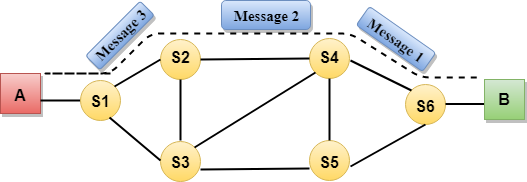
\includegraphics[width=0.8\textwidth]{circuit-switching}
		\caption{Circuit switching}
		\label{fig:circuit-switching}
	\end{center}
\end{figure}
%-------------------FIGURE END----------------------

\textit{Circuits can be permanent or temporary. Applications which use circuit switching may have to go through three phases:}

\begin{multicols}{3}
	\begin{enumerate}[label=\alph*.]
		\item Establish a circuit
		\item Transfer the data
		\item Disconnect the circuit
	\end{enumerate}
\end{multicols}



\begin{multicols}{2}
	\subsubsection*{Advantages}
	\begin{itemize}
		\item In the case of Circuit Switching technique, the communication channel is dedicated.
		\item It has fixed bandwidth.
	\end{itemize}
\end{multicols}



\begin{multicols}{2}
\subsubsection*{Disadvantages}
	\begin{itemize}
		\item Once the dedicated path is established, the only delay occurs in the speed of data transmission.
		\item It takes a long time to establish a connection approx 10 seconds during which no data can be transmitted.
		\item It is more expensive than other switching techniques as a dedicated path is required for each connection.
		\item It is inefficient to use because once the path is established and no data is transferred, then the capacity of the path is wasted.
		\item In this case, the connection is dedicated therefore no other data can be transferred even if the channel is free.
	\end{itemize}
\end{multicols}


\subsection{Message Switching}
\begin{multicols}{2}
	\begin{itemize}
		\item This technique was somewhere in the middle of circuit switching and packet switching.
		\item In message switching, the whole message is treated as a data unit and is switching / transferred in its entirety.
		
		\item A switch working on message switching, first receives the whole message and buffers it until there are resources available to transfer it to the next hop.
		\item If the next hop is not having enough resource to accommodate large size message, the message is stored and switch waits.
		\item This technique was considered substitute to circuit switching.
		\item As in circuit switching, the whole path is blocked for two entities only.
		\item Message switching is replaced by packet switching.
	\end{itemize}
\end{multicols}


%---------------------------------------------------
%
%				FIGURE
%
%---------------------------------------------------
\begin{figure}[pht]
	\begin{center}
		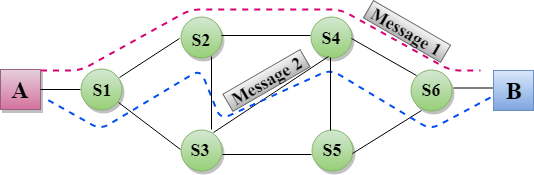
\includegraphics[width=0.8\textwidth]{message-switching}
		\caption{Message switching}
		\label{fig:message-switching}
	\end{center}
\end{figure}
%-------------------FIGURE END----------------------

%Message switching has the following drawbacks:
%\begin{itemize}
%	\item Every switch in transit path needs enough storage to accommodate entire message.
%	\item Because of store-and-forward technique and waits included until resources are available,
%	message switching is very slow.
%	\item Message switching was not a solution for streaming media and real-time applications.
%\end{itemize}


\begin{multicols}{2}
	\subsubsection*{Advantages}
	\begin{itemize}
		\item Data channels are shared among the communicating devices that improve the efficiency of using available bandwidth.
		\item Traffic congestion can be reduced because the message is temporarily stored in the nodes.
		\item Message priority can be used to manage the network.
		\item The size of the message which is sent over the network can be varied. Therefore, it supports the data of unlimited size.
	\end{itemize}
\end{multicols}


\subsubsection*{Disadvantages}
\begin{multicols}{2}
	\begin{itemize}
		\item The message switches must be equipped with sufficient storage to enable them to store the messages until the message is forwarded.
		\item The Long delay can occur due to the storing and forwarding facility provided by the message switching technique.
	\end{itemize}
\end{multicols}



\begin{multicols}{2}
	\subsection{Packet Switching}
	\begin{itemize}
		\item Shortcomings of message switching gave birth to an idea of packet switching.
		\item The entire message is broken down into smaller chunks called packets.
		\item The switching information is added in the header of each packet and transmitted independently.
		\item It is easier for intermediate networking devices to store small size packets, and they do not take much resources either on carrier path or in the internal memory of switches.
		Packet switching enhances line efficiency
		as packets from multiple applications can
		be multiplexed over the carrier.
		\item The Internet uses packet switching technique. Packet switching enables the user to differentiate data streams based on priorities.
		\item Packets are stored and forwarded according to their priority to provide quality of service.
	\end{itemize}
\end{multicols}


%---------------------------------------------------
%				FIGURE
%---------------------------------------------------

\begin{figure}[hpb!]
	\begin{center}
		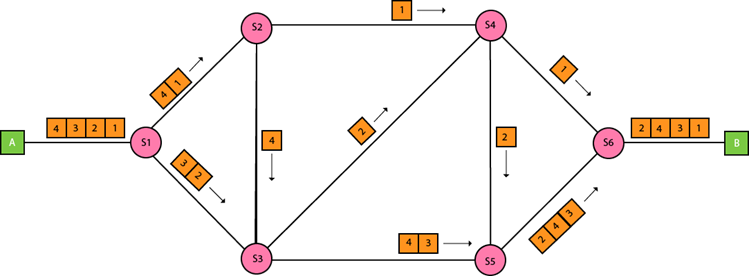
\includegraphics[width=0.8\textwidth]{packet-switching}
		\caption{Packet switching}
		\label{fig:packet-switching}
	\end{center}
\end{figure}
%-------------------FIGURE END----------------------
\raggedbottom

\begin{multicols}{2}
	\subsubsection*{Advantages}
	\begin{itemize}
		\item \textit{Cost-effective}: In packet switching technique, switching devices do not require massive secondary storage to store the packets, so cost is minimized to some extent. Therefore, we can say that the packet switching technique is a cost-effective technique.
		\item \textit{Reliable}: If any node is busy, then the packets can be rerouted. This ensures that the Packet Switching technique provides reliable communication.
		\item \textit{Efficient}: Packet Switching is an efficient technique. It does not require any established path prior to the transmission, and many users can use the same communication channel simultaneously, hence makes use of available bandwidth very efficiently.
	\end{itemize}
\end{multicols}


\begin{multicols}{2}
	\subsubsection*{Disadvantages}
	\begin{itemize}
		\item Packet Switching technique cannot be implemented in those applications that require low delay and high-quality services.
		\item The protocols used in a packet switching technique are very complex and requires high implementation cost.
		\item If the network is overloaded or corrupted, then it requires re-transmission of lost packets. It can also lead to the loss of critical information if errors are not recovered.
	\end{itemize}
\end{multicols}


\begin{table}[hpt!]
	\centering
	\caption{Differences between circuit switching and packet switching}
	\label{tab:circut-vs-packet}
	\begin{center}
		\begin{tabular}{p{5cm}p{5cm}}
		\toprule	
		\textbf{Circuit Switching}	& \textbf{ Packet Switching} \\
		
		\midrule
		Physical path between source and destination	& No physical path\\
		All packets use same path & Packets travels independently \\
		Bandwidth wastage & No bandwidth wastage	\\
		More reliable & Less reliable\\
		No store and forward transmission	& Supports store and forward transmission\\
		\bottomrule
	\end{tabular}
	\end{center}
\end{table}

\section{Wireless Communication Problem}

\subsection{Interference}
\begin{itemize}
	\item Radio transmission cannot be protected against interference using shielding as this is done in coaxial cable or shielded twisted pair. 
	\item For example, electrical engines and lightning cause severe interference and result in higher loss rates for transmitted data or higher bit error rates respectively.
\end{itemize}

\subsection{Regulations and Spectrum}
Frequencies have to be coordinated, and unfortunately, only a very limited amount of frequencies are available  

\subsection{Low Bandwidth}
Transmission rates are very low for wireless devices compared to desktop systems.

\subsection{High Delays}
A serious problem for communication protocols used in today’s Internet (TCP/IP) is the big variation in link characteristics. 

\subsection{Lower Security}
Not only can portable devices be stolen more easily, but the radio interface is also prone to the dangers of eavesdropping.

\subsection{Shared Medium}
Radio access is always realized via a shared medium. As it is impossible to have a separate wire between a sender and each receiver, different competitors have to ‘fight’ for the medium. 

\section{Wireless Network Reference Model}
The architecture of a network defines the protocols and components necessary to satisfy application requirements. One popular standard for illustrating the architecture is the
seven-layer Open System Interconnect (OSI) Reference Model, developed by the International Standards Organization (ISO). OSI specifies a complete set of network functions, grouped into layers, which reside within each network component. The OSI Reference Model is also a handy model for representing the various standards and interoperability of a wireless network.


\begin{figure}[tph]
	\centering
	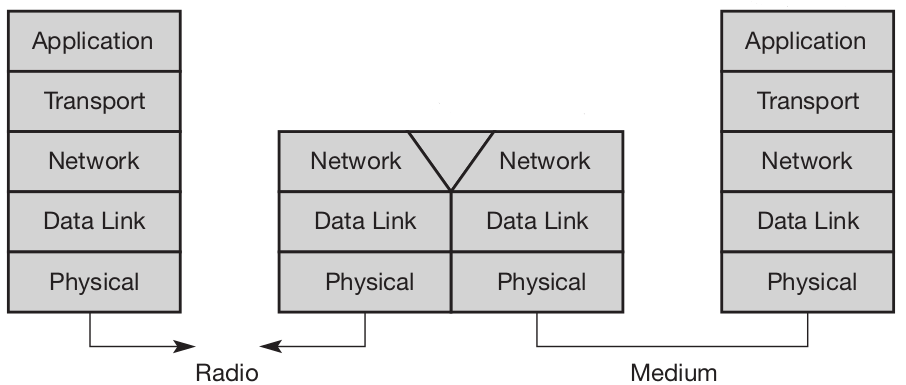
\includegraphics[width=0.8\textwidth]{graphics/wireless-ref-model}
	\caption{Wireless Network Reference Model}
	\label{fig:wireless-ref-model}
\end{figure}



The OSI layers provide the following network functionality:

\subsection*{Layer 7 - Application Layer}
\begin{itemize}
	\item Establishes communications among users and provides basic communications services such as file transfer and e-mail. 
	\item Examples of software that runs at this layer include Simple Mail Transfer Protocol (SMTP), HyperText Transfer Protocol (HTTP) and File Transfer Protocol (FTP).
\end{itemize}


\subsection*{Layer 6 - Presentation Layer} 
\begin{itemize}
	\item Negotiates data transfer syntax for the application layer and performs translations between different data formats, if necessary. 
	\item For example, this layer can translate the coding that represents the data when communicating with a remote system made by a different vendor. 
\end{itemize}


\subsection*{Layer 5 - Session layer}
\begin{itemize}
	\item Establishes, manages, and terminates sessions between applications. Wireless middleware and access controllers provide this form of connectivity over wireless networks. 
	\item If the wireless network encounters interference, the session layer functions will suspend communications until the interference goes away.
\end{itemize}


\subsection*{Layer 4 - Transport Layer}
\begin{itemize}
	\item Provides mechanisms for the establishment, maintenance, and orderly termination of virtual circuits, while shielding the higher layers from the network implementation details. 
	\item In general, these circuits are connections made between network applications from one end of the communications circuit to another (such as between the web browser on a laptop to a web page on a server). 
	\item Protocols such as Transmission Control Protocol (TCP) operate at this layer. 
\end{itemize}


\subsection*{Layer 3 - Network Layer}
\begin{itemize}
	\item Provides the routing of packets though a network from source to destination. 
	\item This routing ensures that data packets are sent in a direction that leads to a particular destination. 
	\item Protocols such as Internet Protocol (IP) operate at this layer.
\end{itemize}


\subsection*{Layer 2 - Data link Layer}
\begin{itemize}
	\item Ensures medium access, as well as synchronization and error control between two entities. 
	\item With wireless networks, this often involves coordination of access to the common air medium and recovery from errors that might occur in the data as it propagates from source to destination. 
	\item Most wireless network types have a common method of performing data link layer functions independent of the actual means of transmission.
\end{itemize}


\subsection*{Layer 1 - Physical Layer}
\begin{itemize}
	\item Provides the actual transmission of information through the medium. 
	\item Physical layers include radio waves and infrared light. 
\end{itemize}

\noindent The combined layers of a network architecture define the functionality of a wireless network, but wireless networks directly implement only the lower layers of the model. A wireless NIC, for example, implements the data link layer and physical layer functions. Other elements of the network (such as wireless middleware), however, offer functions that the session layer implements. In some cases, the addition of a wireless network might impact only the lower layers, but attention to higher layers is necessary to ensure that applications operate effectively in the presence of wireless network impairments. 

Each layer of the OSI model supports the layers above it. In fact, the lower layers often appear transparent to the layers above. For example, TCP operating at the transport layer establishes connections with applications at a distant host computer, without awareness
that lower layers are taking care of synchronization and signaling. 

\section{Wireless Networking Issues \& Standards}

\subsection{Wireless Networking Issues}
\begin{multicols}{2}
%	\begin{itemize}
%		\item Higher loss-rates due to interference (emissions of, e.g., engines, lightning)
%		
%		\item Restrictive regulations of frequencies: frequencies have to be coordinated, useful frequencies are almost all occupied
%		
%		\item Low data transmission rates: local some Mbit/s, regional currently, e.g., 53kbit/s with GSM/ GPRS
%		
%		\item Higher delays, higher jitter: connection setup time with GSM in the second range, several hundred
%		milliseconds for other wireless systems
%		
%		\item Lower security, simpler active attacking: radio interface accessible for everyone, base station can be simulated,
%		thus attracting calls from mobile phones
%		
%		\item Quality of Service (QoS): One of the primary concerns about wireless
%		data delivery is that, unlike the Internet through wired services, QoS is
%		inadequate. Lost packets and atmospheric interference are recurring
%		problems of the wireless protocols.
%		
%		\item Security risk: This is another major issue with a data transfer over a
%		wireless network. Basic network security mechanisms like the service set
%		identifier (SSID) and Wireless Equivalency Privacy (WEP);these measures
%		may be adequate for residences and small businesses, but they are
%		inadequate for the entities that require stronger security.
%	\end{itemize}
\begin{itemize}
	
	\item \textbf{Quality of service}: WLANs typically offer lower quality than their wired counterparts. The main reasons for this are the lower bandwidth due to limitations in radio transmission, and higher delay variation due to extensive error correction and detection mechanisms.
	
	
	
	\item \textbf{Proprietary solutions}: Due to slow standardization procedures, many companies have come up with proprietary solutions offering standardized functionality plus many enhanced features. However, these additional features only work in a homogeneous environment, i.\ e.\ , when adapters from the same vendors are used for all wireless nodes.
	
	
	\item \textbf{Restrictions}: All wireless products have to comply with national regulations. Several government and non-government institutions worldwide regulate the operation and restrict frequencies to minimize interference. WLANs are limited to low-power senders and certain license-free frequency bands, which are not the same worldwide.
	
	\item \textbf{Safety and security}: Using radio waves for data transmission might interfere with other high-tech equipment in, e.\ g.\ , hospitals. Senders and
	receivers are operated by laymen and, radiation has to be low. Special precautions have to be taken to prevent safety hazards. The open radio interface makes eavesdropping much easier in WLANs than, e.\ g.\ , in the case of fiber optics.
	
\end{itemize}
\end{multicols}



\subsection{Wireless Networking Standards}

802.11 represents the IEEE designation for wireless networking. Several wireless networking specifications exist under the 802.11 banner. The 802.11 wireless standards can differ in terms of speed, transmission ranges, and frequency used, but
in terms of actual implementation they are similar. All standards can use either an
infrastructure or ad hoc network design, and each can use the same security
protocols.

\subsubsection*{IEEE 802.11}
\begin{itemize}
	\item There were actually two variations on the initial 802.11 wireless standard.
	\item Both offered $ 1 $ or $ 2Mbps $ transmission speeds and the same RF of $ 2.4GHz $.
	\item The difference between the two was in how data traveled through the RF media. 
	\begin{itemize}
		\item one used FHSS (Frequency Hopping Spread Spectrum), and the 
		\item other used DSSS (Direct Sequence Spread Spectrum). 
	\end{itemize}
	\item The original 802.11 standards are far too slow for modern networking needs and are now no longer deployed.
\end{itemize}

\paragraph*{IEEE 802.11a}
\begin{itemize}
	\item In terms of speed, the 802.11a standard was far ahead of the original 802.11 standards. 
	\item 802.11a specified speeds of up to $ 54Mbps $ in the $ 5GHz $ band.
	\item 802.11a is incompatible with the 802.11b and 802.11g wireless standards.
\end{itemize}

\paragraph*{IEEE 802.11b}
\begin{itemize}
	\item The 802.11b standard provides for a maximum transmission speed of $ 11Mbps $. 
	\item Devices are designed to be backward-compatible with previous 802.11 standards
	\item 802.11b uses a $ 2.4GHz $ RF range and is compatible with 802.11g.
\end{itemize}


\paragraph*{IEEE 802.11g}
\begin{itemize}
	\item 802.11g is a popular wireless standard today. 
	\item 802.11g offers wireless transmission over distances of $ 150 feet $ and speeds up to $  54Mbps $
	\item 802.11g operates in the $ 2.4GHz $ range and therefore is compatible with it.
\end{itemize}


\paragraph*{IEEE 802.11n}
\begin{itemize}
	\item The newest of the wireless standards listed is 802.11n. 
	\item The goal of the 802.11n standard is to significantly increase throughput in both the $ 2.4GHz $ and the $ 5GHz $ frequency range. 
	\item The baseline goal of the standard was to reach speeds of $ 100Mbps $.
	\item Given the right conditions, speeds might reach a $ 600Mbps $. 
	\item In practical operation, 802.11n speeds is much slower.
\end{itemize}



\section{Mobile Computing}
Mobile Computing is a technology that allows transmission of data, voice and video via a computer or any other wireless enabled device without having to be connected to a fixed physical link. 

\subsection{Mobile Communication}
Mobile Communication is a wireless form of communication in which
voice and data information is emitted, transmitted and received via
microwaves. This type of communication allows individuals to
converse with one another and/or transmit and receive data while
moving from place to place. Some examples include: cellular and
digital cordless telephones, pagers, telephone answering devices,
air-to-ground telecommunications and satellite-based
communications.


\subsection{Principles of Mobile Computing}
\begin{itemize}
\item \textbf{Portability}: Devices/nodes connected within the mobile computing
system should facilitate mobility. These devices may have limited
device capabilities and limited power supply, but should have a
sufficient processing capability and physical portability to operate in a
movable environment.

\item \textbf{Connectivity}: This defines the quality of service (QoS) of the network
connectivity. In a mobile computing system, the network availability is
expected to be maintained at a high level with the minimal amount of
lag/downtime without being affected by the mobility of the connected
nodes.

\item \textbf{Interactivity}: The nodes belonging to a mobile computing system are
connected with one another to communicate and collaborate through
active transactions of data.

\item \textbf{Individuality}: A portable device or a mobile node connected to a mobile
network often denote an individual; a mobile computing system should
be able to adopt the technology to cater the individual needs and also
to obtain contextual information of each node.
\end{itemize}



\subsection{Mobile Computing Architecture}
%\begin{figure}[pht]
%	\centering
%	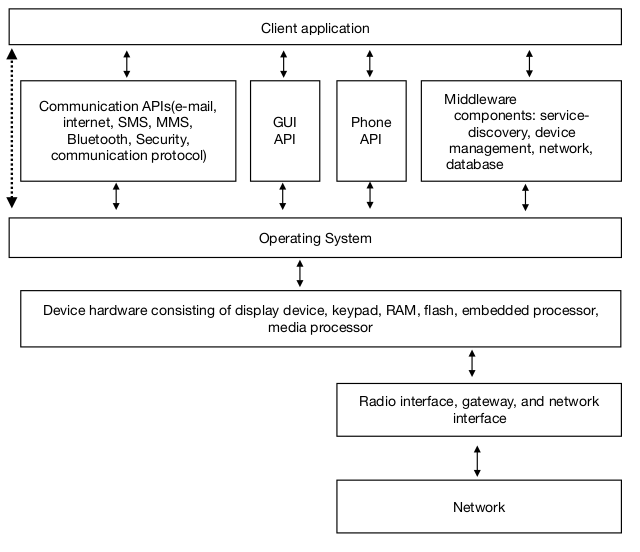
\includegraphics[width=0.8\textwidth]{mobile-computing-architecture}
%	\caption{Mobile Computing Architecture.}
%\end{figure}
The network-centric mobile computing architecture uses three-tier architecture as shown in Figure \ref{fig:3-tier-mobile-computing-architecture}.
\begin{enumerate}
	\item \textit{Tier-1} : Presentation Tier / User interface 
	\item \textit{Tier-2} : Application Tier / Process Management Tier
	\item \textit{Tier-2} : Data Tier / Database Management Tier
\end{enumerate}

%---------------------------------------------------
%				FIGURE
%---------------------------------------------------
\begin{figure}[hpt]
	\begin{center}
		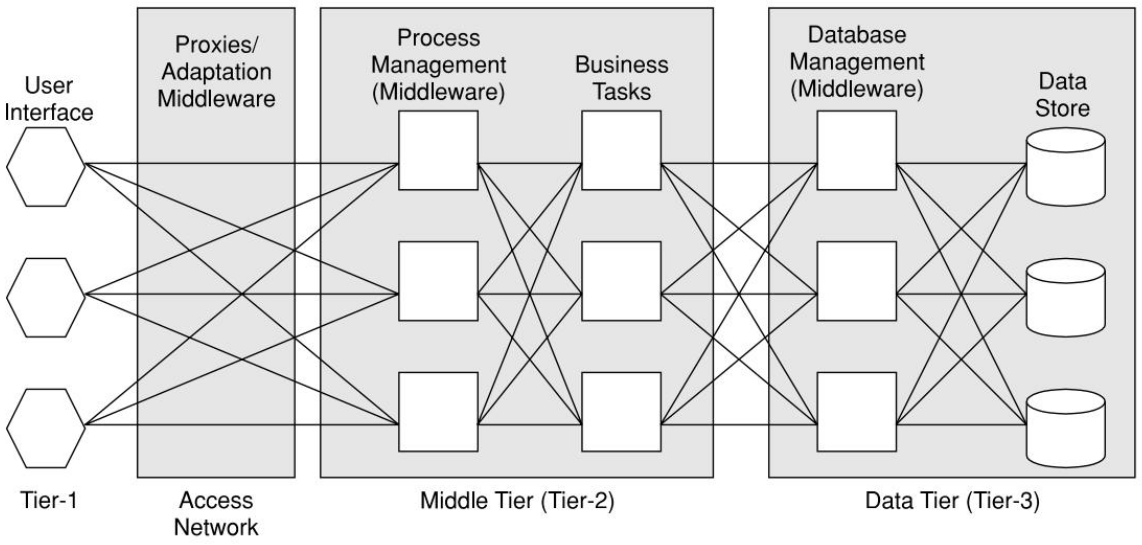
\includegraphics[width=0.9\textwidth]{3-tier-mobile-computing-architecture}
		\caption{Three-tier architecture for mobile computing}
		\label{fig:3-tier-mobile-computing-architecture}
	\end{center}
\end{figure}


\begin{multicols}{2}
	\subsubsection{Presentation Tier}
	\begin{itemize}
		\item This is the user facing system in the first tier. 
		\item This is the layer of agent applications and systems which run on the client device and offer all the user interfaces.
		\item These applications run on the client device and offer all the user interfaces. 
		\item This tier is responsible for presenting the information to the end user.
		\item This tier includes web browsers and customized client programs. 
	\end{itemize}
\end{multicols}


\begin{multicols}{2}
	\subsubsection{Application Tier}
	\begin{itemize}
		\item The application tier or middle tier is the ``engine'' of a ubiquitous application. 
		\item It performs the business logic of processing user input, obtaining data, and making decisions. 
		\item In certain cases, this layer will do the transcoding of data for appropriate rendering in the Presentation Tier. 
	\end{itemize}
\end{multicols}

In addition to the business logic there are quite a few additional management functions that need to be performed. 

Different functions are implemented using different middleware software.
\subsubsection*{Middleware}

A middleware framework is defined as a layer of software, which sits in the middle between the operating system and the user facing software.

Function relate to decisions on: 
\begin{multicols}{2}
	\begin{itemize}
		\item rendering, 
		\item network management, 
		\item security, 
		\item datastore access, etc.
	\end{itemize}
\end{multicols}

Middleware covers a wide range of software systems. We can group middleware into the following major categories:
\begin{multicols}{2}
	\begin{itemize}
		\item Message-oriented Middleware.
		\item Transaction Processing Middleware.
		\item Database Middleware.
		\item Communication Middleware.
		\item Distributed Object and Components.
		\item Transcoding Middleware.
	\end{itemize}
\end{multicols}



\begin{multicols}{2}
	\subsubsection{Data Tier}
	\begin{itemize}
		\item The Data Tier is used to store data needed by the application and acts as a repository for both temporary and permanent data. 
		\item The data can be stored in any form of datastore or database.
		\item These can range from sophisticated relational database, legacy hierarchical database, to even simple text files. 
		\item The data can also be stored in XML format for interoperability with other systems and	data sources. 
	\end{itemize}
\end{multicols}



\subsubsection*{Database Middleware}
Database middleware allows the business logic to be independent and transparent of the database technology and the database vendor.

\begin{multicols}{2}
	\begin{enumerate}
		\item Database middleware runs between the application program and the database. 
		\item These are sometimes called database connectors as well.
		\item Examples of such middleware will be ODBC, JDBC, etc. 
		\item Using these middleware, the application will be able to access data from any data source
	\end{enumerate}
\end{multicols}


\section{Mobile Devices}

Mobile hardware includes mobile devices or device components that receive or access the service of mobility. They would range from portable laptops, smartphones, tablet PCs, Personal Digital Assistants. These devices will have a receptor medium that is capable of sensing and receiving signals. These devices are configured to operate in full-duplex, whereby they are capable of sending and receiving signals at the same time. They don't have to wait until one device has finished communicating for the other device to initiate
communications.

Categories of mobile devices:

\subsection*{Sensor}
A very simple wireless device is represented by a sensor transmitting
state information. 

\subsection*{Embedded Controllers}
Many appliances already contain a simple or sometimes more complex controller. Keyboards, mice, headsets, washing machines, coffee machines, hair dryers and TV sets are just some examples.


\subsection*{Pager}
As a very simple receiver, a pager can only display short text messages, has a tiny display, and cannot send any messages. Pagers can even be integrated into watches.

\subsection*{Mobile phones}
The traditional mobile phone only had a simple black and white text display and could send/receive voice or short messages. Mobile phones with full
color graphic display, touch screen, and Internet browser are available.

\subsection*{Personal digital assistant}
PDAs typically accompany a user and offer
simple versions of office software (calendar, notepad, mail).

\subsection*{Pocket computer}
The next steps toward full computers are pocket computers offering tiny keyboards, color displays, and simple versions of programs found on desktop computers (text processing, spreadsheets etc.).


\subsection*{Tablet}
A tablet computer is a mobile device, a mobile operating system and touchscreen display processing, rechargeable battery in a single, thin and flat package

\subsection*{Notebook/Laptop}
Finally, Laptops offer more or less the same performance as standard desktop computers; they use the same software — the only technical difference being size, weight, and the ability to run on a battery.


%\begin{itemize}
%\item Portable computers, compact, lightweight units including a full character
%set keyboard and primarily intended as hosts for software that may be
%parameterized, such as laptops/desktops, smartphones/tablets, etc.
%
%\item Smart cards that can run multiple applications but are typically used for
%payment, travel and secure area access.
%
%\item Cellular telephones, telephony devices which can call from a distance
%through cellular networking technology.
%
%\item Wearable computers, mostly limited to functional keys and primarily
%intended as incorporation of software agents, such as bracelets,
%keyless implants, etc.
%\end{itemize}

\section{Mobile System Networks}
\begin{multicols}{2}
	\begin{itemize}
		\item Cellular Networks
		\item WLAN Networks
		\item Mobile IP
		\item Ad Hoc Networks
	\end{itemize}
\end{multicols}


\subsection*{Cellular Networks}
\begin{itemize}
\item A cell is the coverage area of a base station, connected to other stations via wire
or fibre or wirelessly through switching centres.
\item The coverage area defines a cell and its boundaries.
\item Each cell base station functions as an access point for the mobile service.
\item Each mobile device connects to the base station of the cell which covers the
current location of the device.
\item All the mobile devices within the range of a given base station communicate with
each other through that base station only.
\end{itemize}

\subsection*{WLAN Networks}
\begin{itemize}
\item WLAN is used for connectivity between the Internet, two LANs, mobile devices, and
computers
\item Mobile device connects to an access point.
\item The access point, in turn, connects to a host LAN which links up to the Internet through a
router
\end{itemize}

\subsection*{Mobile IP}
Mobile IP communication protocol refers to the forwarding of Internet traffic with a fixed IP
address even outside the home network. It allows users having wireless or mobile devices
to use the Internet remotely.
\par

Mobile IP is mostly used in WAN networks, where users need to carry their mobile devices
across different LANs with different IP addresses. Mobile IP is not a wireless protocol.
However, it could be employed for the IP infrastructure of cellular networks.


\subsection*{Ad Hoc Networks}
\begin{itemize}
	\item A wireless ad hoc network (WANET) or MANET (Mobile ad hoc network) is a decentralized type of wireless network. 
	\item The network is ad hoc because it does not rely on	a pre-existing infrastructure, such as routers in wired networks or access points in managed (infrastructure) wireless networks. 
	\item Instead, each node participates in routing by	forwarding data for other nodes, so the determination of which nodes forward data is made dynamically on the basis of network connectivity and the routing algorithm in use. 
	\item Wireless mobile ad hoc networks are self-configuring, dynamic networks in which nodes are free to	move. 
	\item Wireless networks lack the complexities of infrastructure setup and administration, enabling devices to create and join networks ``on the fly” — anywhere, anytime.
\end{itemize}


\section{Mobility Management}
Mobility management is a functionality that facilitates mobile device operations in Universal Mobile Telecommunications System (UMTS) or Global System for Mobile Communications
(GSM) networks. Mobility management is used to trace physical user and subscriber locations to provide mobile phone services, like calls and Short Message Service (SMS).\par 


Mobility management contains two components: 
\begin{enumerate}
	\item location management and 
	\item handoff management
\end{enumerate}

\subsection*{Location Management}
 Location management enables the system to track the attachment points of MTs (Mobile Terminals) between consecutive communications. 


\subsection*{Handoff}
Handoff (or handover) management enables the network to maintain a user’s connection as the MT continues to move and change its access point to the network. Moreover, when a user is in the coverage area of multiple wireless networks, for example, in heterogeneous wireless environments, handoff management provides always best connectivity to the user by connecting the user to the best available network. \par


\noindent Mobility in wireless networks can take different forms, such as:
\begin{itemize}
\item \textbf{Terminal mobility}: the ability for a user terminal to continue to access the network when the terminal moves;
\item \textbf{User mobility}: the ability for a user to continue to access network services from different terminals under the same user identity when the user moves;
\item \textbf{Service mobility}: the ability for a user to access the same services regardless of where the user is.
\end{itemize}

\newpage\thispagestyle{empty} % Chapter-1: Wireless Networks
% !TeX root = ../wireless_networks.tex
\chapter{Wireless LAN}
Some advantages of WLAN are:

\begin{itemize}
\item \textbf{Flexibility}: Within radio coverage, nodes can communicate without further
restriction. Radio waves can penetrate walls, senders and receivers can be
placed anywhere (also non-visible, e.\ g.\ , within devices, in walls etc.).


\item \textbf{Planning}: Only wireless ad-hoc networks allow for communication without previous planning, any wired network needs wiring plans. As long as devices follow the same standard, they can communicate. 

\item \textbf{Design}: Wireless networks allow for the design of small, independent devices which can for example be put into a pocket. Wireless senders and receivers can be hidden in historic buildings,  e.\ g.\ , current networking technology can be introduced without being visible.


\item \textbf{Robustness}: Wireless networks can survive disasters, e.\ g.\ , earthquakes or users pulling a plug. If the wireless devices survive, people can still communicate. 

\item \textbf{Cost}: After providing wireless access to the infrastructure via an access point for the first user, adding additional users to a wireless network will not
increase the cost. This is, important for  e.\ g.\ , lecture halls, hotel lobbies or gate areas in airports where the numbers using the network may vary significantly. 
\end{itemize}


\section{Infrared Vs Radio Transmission}
Two different basic transmission technologies can be used to set up WLANs. One technology is based on the transmission of \textit{infrared light} ( e.\ g.\ , at 900 nm
wavelength), the other one, which is much more popular, uses \textit{radio transmission} in the GHz range ( e.\ g.\ , 2.4 GHz in the license-free ISM band). Both technologies
can be used to set up ad-hoc connections for work groups, to connect,  e.\ g.\ , a desktop with a printer without a wire, or to support mobility within a small area.


\subsection{Infrared Transmission}
\begin{itemize}
	\item Infrared technology uses diffuse light reflected at walls, furniture etc.\ or directed light if a line-of-sight (LOS) exists between sender and receiver. 
	\item Senders can be simple light emitting diodes (LEDs) or laser diodes. 
	\item Photodiodes act as receivers.
\end{itemize}

\begin{multicols}{2}
	\subsubsection*{Advantages}
	\begin{itemize}
		\item The main advantages of infrared technology are its simple and extremely cheap senders and receivers which are integrated into nearly all mobile devices available today. For example, PDAs, laptops, notebooks, mobile phones etc.\ have
		an infra-red data association (IrDA) interface. 
		\item No licenses are needed for infrared technology and shielding is very simple. 
		\item Electrical devices do not interfere with infrared transmission.
	\end{itemize}
\end{multicols}




\begin{multicols}{2}
	\subsubsection*{Disadvantages}
	\begin{itemize}
		\item Disadvantages of infrared transmission are its low bandwidth compared to	other LAN technologies. 
		\item Typically, IrDA devices are internally connected to a serial port limiting transfer rates to 115 kbit/s. 
		\item However, their main disadvantage is that infrared	is quite easily shielded. 
		\item Infrared transmission cannot penetrate walls or other obstacles. 
		\item Typically, for good transmission quality and high data rates a LOS, i.\ e.\, direct connection, is needed.
	\end{itemize}
\end{multicols}

\subsection{Radio Transmission}
HIPERLAN and Bluetooth rely on radio transmission.

\begin{multicols}{2}
\subsubsection*{Advantages}
	\begin{itemize}
		\item Advantages of radio transmission include the long-term experiences made with radio transmission for wide area networks (e.\ g.\ , microwave links) and mobile cellular phones. 
		\item Radio transmission can cover larger areas and can	penetrate (thinner) walls, furniture, plants etc. 
		\item Additional coverage is gained by reflection. 
		\item Radio typically does not need a LOS if the frequencies are not too high. 
		\item Furthermore, current radio-based products offer much	higher transmission rates than infrared.
	\end{itemize}
\end{multicols}



The main advantage is also a big disadvantage of radio transmission.
\begin{multicols}{2}
	\subsubsection*{Disadvantages}
\begin{itemize}
	\item Shielding is not so simple. 
	\item Radio transmission can interfere with other senders, or electrical devices can destroy data transmitted via radio.
	\item Additionally, radio transmission is only permitted in certain frequency bands. 
	\item Very limited ranges of license-free bands are available worldwide and	those that are available are not the same in all countries.
\end{itemize}
\end{multicols}


\section{Infrastructure and Ad-hoc Network}\label{sec:infrastructure-ad-hoc}

\subsection{Infrastructure Network}
Many WLANs of today need an infrastructure network. Infrastructure networks not only provide access to other networks, but also include forwarding functions, medium access control etc. 
\begin{itemize}
	\item In these infrastructure-based wireless networks, communication typically takes place only between the wireless nodes and the access point (see Figure \ref{fig:ad-hoc-network}), but not directly between the wireless nodes.
	\item The access point does not just control medium access, but also acts as a bridge to other wireless or wired networks. Figure \ref{fig:ad-hoc-network} shows three access points with their three wireless networks and a wired network. 
	\item Several wireless networks may form one logical wireless network, so the access points together with the fixed network in between can connect several wireless networks to form a larger network beyond actual radio coverage.
	
\end{itemize}


%--------------------------------------------
%				
%				Figure
%
%--------------------------------------------

\begin{figure}[pht]
\centering
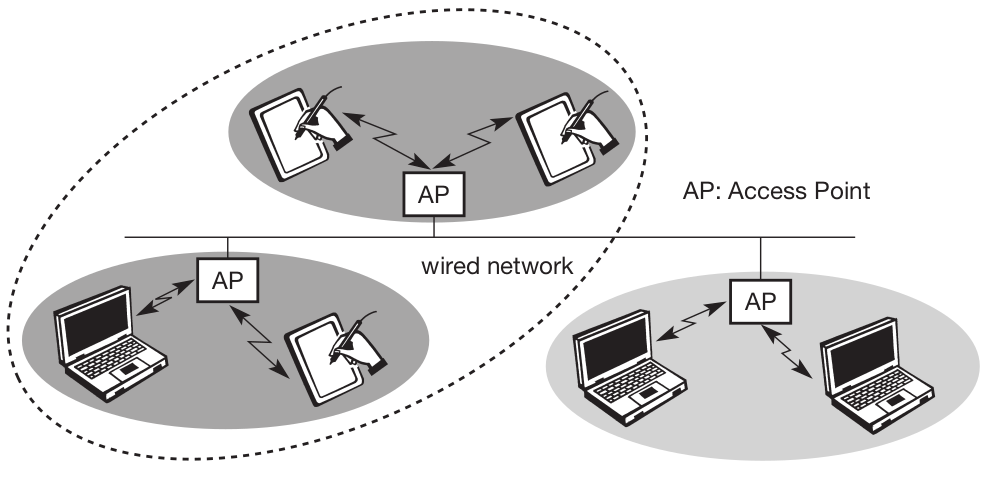
\includegraphics[width=0.8\textwidth]{ad-hoc-network}
\caption{Example of three infrastructure-based wireless networks}\label{fig:ad-hoc-network}
\end{figure}
\subsubsection*{Advantages}
\begin{itemize}
	\item The design of infrastructure-based wireless networks is simpler because most of the network functionality lies within the access point, whereas the wireless clients can remain quite simple. 
	\item If only the access point controls medium access, no collisions are possible. 
	\item This setting may be useful for quality of service guarantees such as minimum bandwidth for certain nodes. 
	\item The access point may poll the single wireless nodes to ensure the data rate.
\end{itemize}

\subsubsection*{Disadvantage(s)}

\begin{itemize}
	\item Infrastructure-based networks lose some of the flexibility wireless networks can offer, e.\ g.\ , they cannot be used for disaster relief in cases where no infrastructure is left. 
\end{itemize}

\noindent Typical cellular phone networks are infrastructure-based networks for a wide area. Also satellite-based cellular phones have an infrastructure - the satellites. Infrastructure does not necessarily imply a wired fixed network.


\subsection{Ad-hoc Network}
\begin{itemize}
	\item Ad-hoc wireless networks, however, do not need any infrastructure to work. 
	\item Each node can communicate directly with other nodes, so no access point controlling medium access is necessary. 
	
\end{itemize}

Figure {\ref{fig:two-ad-hoc-wireless-networks}} shows two ad-hoc networks with three nodes each. Nodes within an ad-hoc network can only communicate if they can reach each other physically, i.\ e.\ , if they are within each other’s radio range or if other nodes can forward the message. Nodes from the two networks shown in Figure {\ref{fig:two-ad-hoc-wireless-networks}} cannot, therefore, communicate with each other if they are not within the same radio range.

%%%%%%%%%%%%%%%%%%%%%%%%%%%%%%%%%%%%%%%%%%%%%%
%				
%				Figure
%
%%%%%%%%%%%%%%%%%%%%%%%%%%%%%%%%%%%%%%%%%%%%%%
\begin{figure}[pht!]
	\centering
	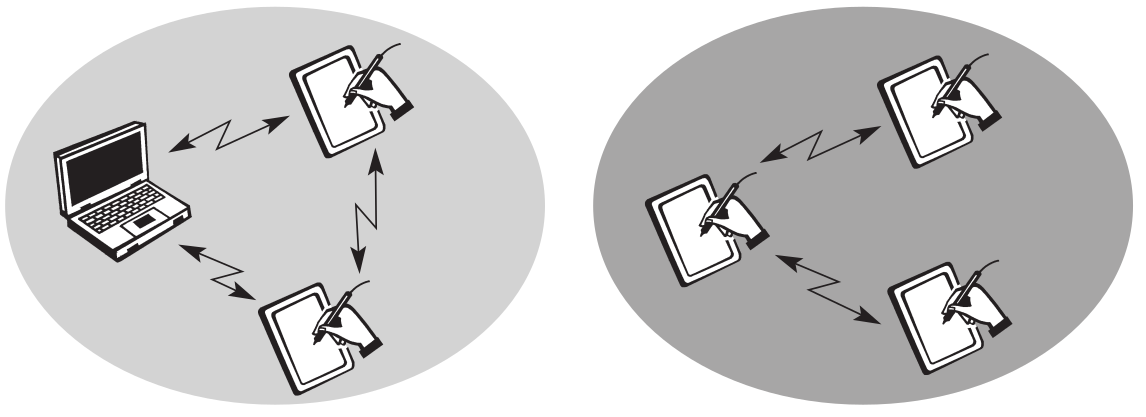
\includegraphics[width=0.8\textwidth]{two-ad-hoc-wireless-networks}
	\caption{Example of two ad-hoc wireless networks}\label{fig:two-ad-hoc-wireless-networks}
\end{figure}

\subsubsection*{Advantage}
\begin{itemize}
	\item This type of wireless network exhibits the greatest possible flexibility as it is, for example, needed for unexpected meetings, quick replacements of infrastructure or communication scenarios far away from any infrastructure.
\end{itemize}
\subsubsection*{Disadvantage}
\begin{itemize}
	\item The complexity of each node is higher because every node has to implement medium access mechanisms, mechanisms to handle hidden or exposed terminal problems, and perhaps priority mechanisms, to provide a certain quality of service.
\end{itemize}




\section{IEEE 802.11}
The IEEE standard 802.11 specifies the most famous family of WLANs in which many products are available. This standard belongs to the group of 802.x LAN standards,  e.\ g.\ , 802.3 Ethernet or 802.5 Token Ring.

The primary goal of the standard was the specification of a simple and robust WLAN which offers time-bounded and asynchronous services. The MAC layer should be able to operate with multiple physical layers, each of which exhibits a different medium sense and transmission characteristic. Candidates for physical layers were infrared and spread spectrum radio transmission techniques.

Additional features of the WLAN should include the support of power management to save battery power, the handling of hidden nodes, and the ability to operate worldwide. The 2.4 GHz ISM band, which is available in most countries around the world, was chosen for the original standard. Data rates envisaged for the standard were 1 Mbit/s mandatory and 2 Mbit/s optional.

\subsection{System Architecture}\label{sec:wireless-network-architecture}
Wireless networks can exhibit two different basic system architectures as shown
in section {\ref{sec:infrastructure-ad-hoc}}: \textit{infrastructure-based} or \textit{ad-hoc}. Figure {\ref{fig:architecture-of-ieee-802-11}} shows the components of an infrastructure and a wireless part as specified for IEEE 802.11. 

%%%%%%%%%%%%%%%%%%%%%%%%%%%%%%%%%%%%%%%%%%%%%%
%				
%				Figure
%
%%%%%%%%%%%%%%%%%%%%%%%%%%%%%%%%%%%%%%%%%%%%%%
\begin{figure}[hpt!]
	\centering
	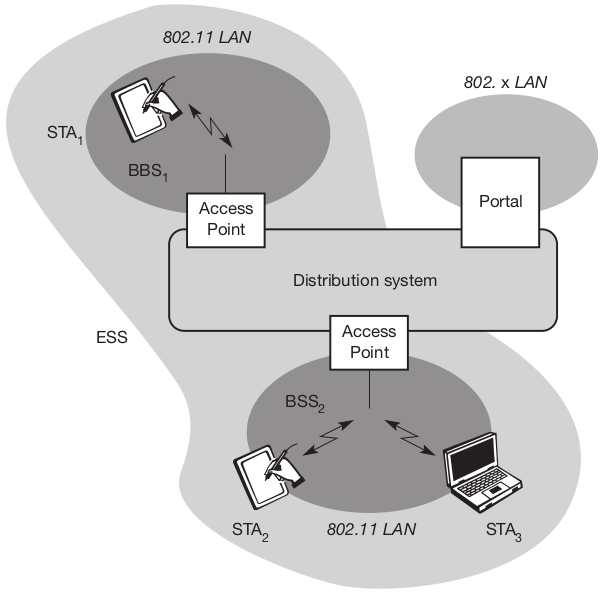
\includegraphics[width=0.7\textwidth]{architecture-of-ieee-802-11}
	\caption{Architecture of an infrastructure-based IEEE 802.11}\label{fig:architecture-of-ieee-802-11}
\end{figure}


\subsubsection[AP]{Access Point (AP)}
Several nodes, called \textbf{stations} ($STA_{i}$), are connected to \textbf{access points (AP)}.

\subsubsection[STA]{Stations (STA)}
 \textbf{Stations} are terminals with access mechanisms to the wireless medium and radio contact to the AP. 

\subsubsection[BSS]{Basic Service Set (BSS)}
The stations and the AP which are within the same radio coverage form a \textbf{basic service set} ($BSS_{i}$). The example shows two BSSs --- $ BSS_1 $ and $ BSS_2 $ --- which are connected via a distribution system. 

\subsubsection[ESS]{Extended Service Set (ESS)}
A distribution system connects several BSSs via the AP to form a single network and thereby extends the wireless coverage area. This network is now called an \textbf{extended service set (ESS)} and has its own identifier, the ESSID. The ESSID is the `name' of a network and is used to separate different networks. Without knowing the ESSID (and assuming no hacking) it should not be possible to participate in the WLAN. 

\subsubsection[Portal]{Portal}
The distribution system connects the wireless networks via the APs with a portal, which forms the interworking unit to other LANs.


\noindent The architecture of the distribution system is not specified further in IEEE 802.11. It could consist of bridged IEEE LANs, wireless links, or any other networks. However, \textbf{distribution system} services are defined in the standard

\subsubsection{Distribution System}
Stations can select an AP and associate with it. The APs support roaming (i.\ e.\ , changing access points), the distribution system handles data transfer between the different APs. 
\begin{itemize}
	\item APs provide synchronization within a BSS, 
	\item support power management, and 
	\item can control medium access to support time-bounded service. 
\end{itemize}


\noindent In addition to infrastructure-based networks, IEEE 802.11 allows the building of ad-hoc networks between stations, thus forming one or more independent BSSs (IBSS) as shown in Figure {\ref{fig:ad-hoc-wlan-architecture}}. In this case, an IBSS comprises a group of stations using the same radio frequency. Stations $STA_1$, $ STA_2 $, and $ STA_3 $ are in $ IBSS_1 $, $ STA_4 $ and $ STA_5 $ in $ IBSS_2 $. This means for example that $ STA_3 $ can communicate directly with $ STA_2 $ but not with $ STA_5 $. Several IBSSs can either be formed via the distance between the IBSSs (see Figure {\ref{fig:ad-hoc-wlan-architecture}}) or by using different carrier frequencies (then the IBSSs could overlap physically). 

%%%%%%%%%%%%%%%%%%%%%%%%%%%%%%%%%%%%%%%%%%%%%%
%				
%				Figure
%
%%%%%%%%%%%%%%%%%%%%%%%%%%%%%%%%%%%%%%%%%%%%%%
\begin{figure}[phb!]
	\centering
	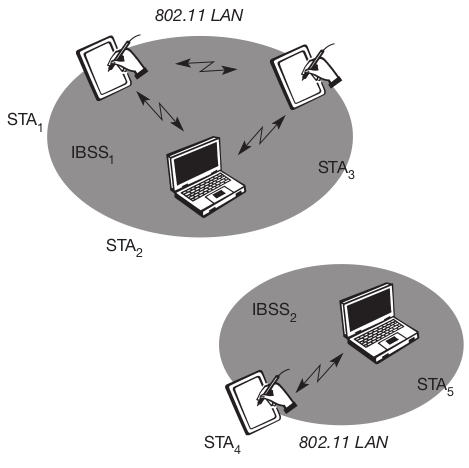
\includegraphics[width=0.7\textwidth]{ad-hoc-wlan-architecture}
	\caption{Architecture of IEEE 802.11 ad-hoc wireless LANs}\label{fig:ad-hoc-wlan-architecture}
\end{figure}

\subsection{Protocol Architecture}
IEEE 802.11 fits seamlessly into the other 802.x standards for wired LANs. Figure \ref{fig:ieee-802-11-protocol-architecture} shows the most common scenario: 
%\begin{multicols}{2}
	\begin{enumerate}
		\item An IEEE 802.11 wireless LAN connected to a switched IEEE 802.3 Ethernet via a bridge. 
		\item Applications should not notice any difference apart from the lower bandwidth and perhaps higher access time from the wireless LAN. 
		\item The WLAN behaves like a slow wired LAN. 
		\item Consequently, the higher layers (application, TCP, IP) look the same for wireless nodes as for wired nodes. 
		\item The upper part of the data link control layer, the logical link control (LLC), covers the differences of the medium access control layers needed for the different media.  
	\end{enumerate}
%\end{multicols}

%%%%%%%%%%%%%%%%%%%%%%%%%%%%%%%%%%%%%%%%%%%%%%
%				
%				Figure
%
%%%%%%%%%%%%%%%%%%%%%%%%%%%%%%%%%%%%%%%%%%%%%%
\begin{figure}[pht]
	\centering
	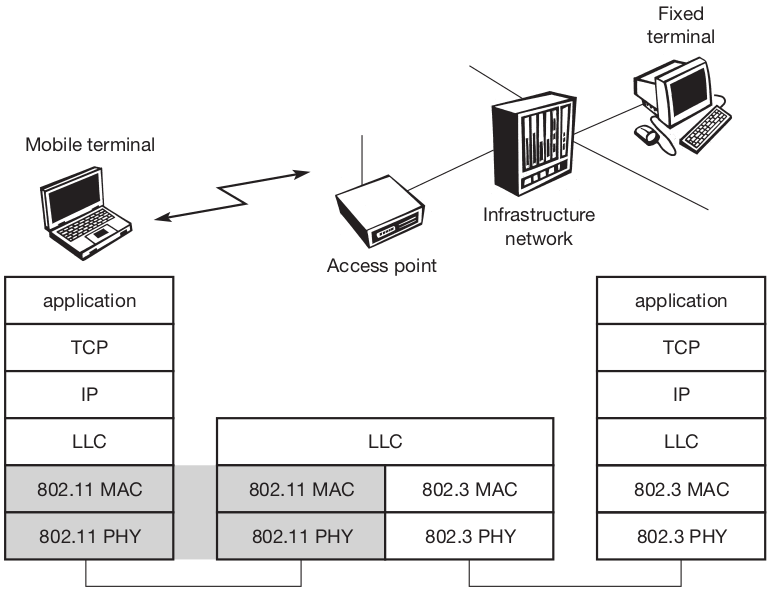
\includegraphics[width=0.8\textwidth]{ieee-802-11-protocol-architecture}
	\caption{IEEE 802.11 protocol architecture and bridging}\label{fig:ieee-802-11-protocol-architecture}
\end{figure}

In many of today’s networks, no explicit LLC layer is visible.



The IEEE 802.11 standard only covers the physical layer \textbf{PHY} and medium access layer \textbf{MAC} like the other 802.x LANs do.
%%%%%%%%%%%%%%%%%%%%%%%%%%%%%%%%%%%%%%%%%%%%%%
%				
%				Figure
%
%%%%%%%%%%%%%%%%%%%%%%%%%%%%%%%%%%%%%%%%%%%%%%

\begin{figure}[h!]
	\centering
	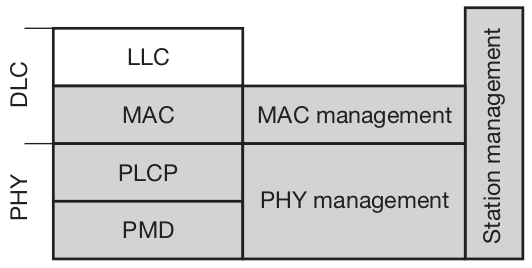
\includegraphics[width=0.8\textwidth]{ieee-802-11-protocol-architecture-and-management}
	\caption{Detailed IEEE 802.11 protocol architecture and management}\label{fig:ieee-802-11-protocol-architecture-and-management}
\end{figure}

\subsubsection[PHY]{Physical Layer}
 The physical layer is subdivided into:
 \begin{enumerate}
 	\item \textbf{physical layer convergence protocol (PLCP)} and 
 	\item \textbf{physical medium dependent} (\textbf{PMD}) sublayer (see Figure \ref{fig:ieee-802-11-protocol-architecture-and-management}). 
 \end{enumerate}


\paragraph{PLCP}
\begin{itemize}
	\item The PLCP sublayer provides a carrier sense signal, called clear \textit{channel assessment (CCA)}, and 
	\item provides a common PHY service access point (SAP) independent of the transmission technology. 
	\item Finally, the PMD sublayer handles modulation and encoding/decoding of signals. 
\end{itemize}


\subsubsection[MAC]{MAC Layer}
The basic tasks of the MAC layer comprise:
\begin{itemize}
	\item medium access, 
	\item fragmentation of user data, and 
	\item encryption.
\end{itemize}


\noindent Apart from the protocol sublayers, the standard specifies \textbf{management layers} and the \textbf{station management}. 

\subsubsection*{MAC Management}
\begin{itemize}
	\item The MAC management supports the association and re-association of a station to an access point and roaming between different access points. 
	\item It also controls authentication mechanisms, encryption, synchronization of a station with regard to an access point, and power management to save battery power. 
	\item MAC management also maintains the MAC	management information base (MIB).
\end{itemize}



\subsubsection*{PHY Management}
The main tasks of the PHY management include channel tuning and PHY MIB maintenance. 

\subsubsection*{Station Management}
Station management interacts with both management layers and is responsible for additional higher layer functions (e.\ g.\ , control of bridging and interaction with the distribution system in the case of an access point).



\subsection{802.11b}\label{sec:802.11b}

Soon after the first commercial 802.11 products came on the market some companies offered proprietary solutions. To avoid market
segmentation, a common standard, \textbf{IEEE 802.11b}\footnote{Do not
	get confused about the fact that 802.11b hit the market before 802.11a. The
	standards are named according to the order in which the respective study
	groups have been established.} soon followed and was added as supplement to the original standard (Higher-speed physical layer extension in the 2.4 GHz band). 


\begin{itemize}
	\item This standard describes a new PHY layer.
	\item Depending on the interference and the distance between sender and receiver 802.11b systems offer $ 11 $, $ 5.5 $, $ 2 $, or $ 1 Mbit/s $. 
	\item Maximum user data rate is approx $ 6 Mbit/s $.
	\item The standard defines several packet formats for the physical layer.
	\item The mandatory format interoperates with the original versions of 802.11. 
	\item The optional versions provide a more efficient data transfer due to shorter headers/different coding schemes and can coexist with other 802.11 versions.
	\item The standards operates on certain frequencies in the 2.4 GHz ISM band. These depend on national regulations.
	\item Devices using 802.11b experience interference from other products operating in the 2.4 GHz band.
	\item \textbf{Pros of 802.11b}: lowest cost; signal range is good and not easily obstructed.
	\item \textbf{Cons of 802.11b}: slowest maximum speed; home appliances may interfere on the unregulated frequency band.
\end{itemize}


\subsection{802.11a} \label{sec:802.11a}
While 802.11b was in development, IEEE created a second extension to the original 802.11 standard called 802.11a. Because 802.11b gained in popularity much faster than did 802.11a.

\begin{itemize}
	\item Uses the same data link layer protocol and frame format as the original standard, but an OFDM\footnote{orthogonal frequency-division multiplexing (OFDM) is a type of digital transmission and a method of encoding digital data on multiple carrier frequencies.} based air interface (physical layer).
	\item It operates in the 5 GHz band with a maximum net data rate of $ 54 Mbit/s $.
	\item The higher frequency also means 802.11a signals have more difficulty penetrating walls and other obstructions.
	\item Because 802.11a and 802.11b utilize different frequencies, the two technologies are incompatible with each other. 
	\item \textbf{Pros of 802.11a}: fast maximum speed; regulated frequencies prevent signal interference from other devices.
	\item \textbf{Cons of 802.11a}: highest cost; shorter range signal that is more easily obstructed.
\end{itemize}


\subsection{Newer Developments} \label{sec:newer-developments}
While many products that follow the IEEE 802.11a and 802.11b standards are available, several new groups have been formed within the IEEE to discuss enhancements of the standard and new applications.

\begin{itemize}
\item \textbf{802.11e (MAC enhancements)}: For applications such as audio, video, or media stream, distribution service classes have to be provided. For this
reason, the MAC layer must be enhanced compared to the current standard.

\item \textbf{802.11f (Inter-Access Point Protocol)}: The standard currently only describes the basic architecture of 802.11 networks and their components. 

\item \textbf{802.11g (Data rates above 20 Mbit/s at 2.4 GHz)}: Introducing new modulation schemes, forward error correction and OFDM also allows for higher data
rates at 2.4 GHz. This approach should be backward compatible to 802.11b
and should benefit from the better propagation characteristics at 2.4 GHz compared to 5 GHz.

\item \textbf{802.11h (Spectrum managed 802.11a)}: The 802.11a standard was primarily designed for usage in the US U-NII bands. The standardization did not consider non-US regulations such as the European requirements for power control and dynamic selection of the transmit frequency. To enable the regulatory acceptance of 5 GHz products, dynamic channel selection (DCS) and transmit power control (TPC) mechanisms (as also specified for the European HiperLAN2 standard) have been added. With this extension, 802.11a products can also be operated in Europe. These additional mechanisms try to balance the load in the 5 GHz band.

\item \textbf{802.11i (Enhanced Security mechanisms)}: As the original security mechanisms (WEP) proved to be too weak soon after the deployment of the first products, this working group discusses stronger encryption and authentication mechanisms. IEEE 802.1x will play a major ⎄role in this process.
\end{itemize}

\subsection{HIPERLAN 1} \label{sec:hiperlan-1}
In 1996, the ETSI standardized HIPERLAN 1 as a WLAN allowing for node mobility and supporting ad-hoc and infrastructure-based topologies. (HIPERLAN stands for \textbf{high performance local area network}.) \textbf{HIPERLAN 1} was originally one out of four HIPERLANs envisaged, as ETSI decided to have different types of networks for different purposes. The key feature of all
four networks is their integration of time-sensitive data transfer services. Over time, names have changed and the former HIPERLANs 2, 3, and 4 are now called HiperLAN2, HIPERACCESS, and HIPERLINK.

The service offered by a HIPERLAN 1 is compatible with the standard MAC services known from IEEE 802.x LANs

An innovative feature of HIPERLAN 1, which many other wireless networks do not offer, is its ability to forward data packets using several relays. Relays can extend the communication on the MAC layer beyond the radio range.

HiperLAN features:

\begin{itemize}
	\item range $ 100 m $
\item slow mobility ($ 1.4 m/s $)
\item supports asynchronous and synchronous traffic
\item Bit rate - $ 23.59 Mbit/s $
\end{itemize}


\subsection{HIPERLAN 2} \label{sec:hiperlan-2}
While HIPERLAN 1 did not succeed HiperLAN2 might have a better chance. (This is also written as HIPERLAN/2, HiperLAN/2, H/2) Standardized by ETSI this wireless network works at 5 GHz  and offers data rates of up to $ 54 Mbit/s $ including QoS support and enhanced security features. In comparison with basic IEEE 802.11 LANs, HiperLAN2 offers more features in the mandatory parts
of the standard.

Features:

\subsubsection*{High-throughput transmission}
\begin{itemize}
	\item HiperLAN2 not only offers up to $ 54 Mbit/s $ at the physical layer but also about $ 35 Mbit/s $ at the network layer.
	\item The overheads introduced by the layers (medium access, packet headers etc.) remain almost constant over a wide range of user packet sizes and Data rates.
\end{itemize}

\subsubsection*{Connection-oriented}
Prior to data transmission HiperLAN2 networks establish logical connections between a sender and a receiver.


\subsubsection*{Quality of service support}
With the help of connections, support of QoS is much simpler. Each connection has its own set of QoS parameters.

\subsubsection*{Dynamic frequency selection}
\begin{itemize}
	\item HiperLAN2 does not require frequency planning.
	\item All access points have built-in support which automatically selects an appropriate frequency within their coverage area.
\end{itemize}

\subsubsection*{Security support}
Authentication as well as encryption is supported by HiperLAN2.

\subsubsection*{Mobility support}
\begin{itemize}
	\item Mobile terminals can move around while transmission always takes place between the terminal and the access point with the best radio signal.
	\item Handover between access points is performed automatically.
\end{itemize}

\section{Bluetooth} \label{sec:bluetooth}
Compared to the WLAN technologies, the Bluetooth technology aims at so-called \textbf{ad-hoc piconets}, which are local area networks with a very limited coverage and without the need for an infrastructure. This is a different type of network is needed to connect different
small devices in close proximity (about 10 m) without expensive wiring or the need for a wireless infrastructure. 

Swedish IT-company Ericsson initiated some studies in 1994 around a so-called multi-communicator link. The project was renamed and Bluetooth was born. In spring 1998 five companies (Ericsson, Intel, IBM, Nokia, Toshiba) founded the Bluetooth consortium with the goal of developing a single-chip, low-cost, radio-based wireless network technology. Many other companies and research institutions joined the special interest group around Bluetooth, whose goal was the development of mobile phones, laptops, notebooks, headsets etc. including Bluetooth technology, by the end of 1999. 

In 2001, the first products hit the mass market, and many mobile phones, laptops, PDAs, video cameras etc. are equipped with Bluetooth technology today.


\subsection{User Scenarios}
Many different user scenarios can be imagined for wireless piconets or WPANs:

\begin{itemize}
\item \textbf{Connection of peripheral devices}: Today, most devices are connected to a desktop computer via wires (e.\ g.\ , keyboard, mouse, joystick, headset, speakers). This type of connection has several disadvantages: each device has its
own type of cable, different plugs are needed, wires block office space. In a
wireless network, no wires are needed for data transmission. However, batteries now have to replace the power supply, as the wires not only transfer
data but also supply the peripheral devices with power.

\item \textbf{Support of ad-hoc networking}: Imagine several people coming together,
discussing issues, exchanging data (schedules, sales figures etc.). For
instance, students might join a lecture, with the teacher distributing data to
their personal digital assistants (PDAs). Wireless networks can support this
type of interaction; small devices might not have WLAN adapters following
the IEEE 802.11 standard, but cheaper Bluetooth chips built in.

\item \textbf{Bridging of networks}: Using wireless piconets, a mobile phone can be connected to a PDA or laptop in a simple way. Mobile phones have a Bluetooth chip. The mobile phone
can then act as a bridge between the local piconet and, e.\ g.\ , the global GSM
network. 
\end{itemize}

When comparing Bluetooth with other WLAN technology we have to keep
in mind that one of its goals was to provide local wireless access at very low
cost. From a technical point of view, WLAN technologies like those above could
also be used, however, WLAN adapters, e.\ g.\ , for IEEE 802.11, have been
designed for higher bandwidth and larger range and are more expensive and
consume a lot more power.

\subsection{Architecture} \label{sec:bluetooth-architecture}
Like IEEE 802.11b, Bluetooth operates in the 2.4 GHz ISM band. However, MAC, physical layer and the offered services are completely different.

\subsubsection*{Networking}
Bluetooth operates on 79 channels in the 2.4 GHz band with 1 MHz carrier spacing. Each device performs frequency hopping with
1,600 hops/s in a pseudo random fashion. 

A very important term in the context of Bluetooth is a \textbf{piconet}. 

\subsubsection{Piconet}
A piconet is a collection of Bluetooth devices which are synchronized to the same hopping
sequence. Figure {\ref{fig:bluetooth-piconet}} shows a collection of devices with different roles.
\begin{enumerate}
	\item One device in the piconet can act as \textbf{master} (M) all other devices connected to the master must act as \textbf{slaves} (S)
	\item The master determines the hopping pattern in the piconet and the slaves have to synchronize to this pattern.
	\item Each piconet has a unique hopping pattern. If a device wants to participate it has to synchronize to
	this.
	\item Two additional types of devices are shown: 
	\begin{itemize}
		\item \textbf{parked devices} (P) can not actively participate in the piconet (e.\ g.\ , they do not have a connection), but are
		known and can be reactivated within some milliseconds.
		\item Devices in \textbf{stand-by} (SB) do not participate in the piconet.
	\end{itemize}
\end{enumerate}

\begin{multicols}{2}
	\begin{itemize}
		\item Each piconet has exactly one master and up to seven simultaneous slaves. 
		\item More than 200 devices can be parked. 
		\item The reason for the upper limit of eight active devices, is the 3-bit address used in Bluetooth. 
		\item If a parked device wants to communicate and there are already seven active slaves, one slave has to switch to park mode to allow the parked device to switch to active mode.
	\end{itemize}
\end{multicols}


%%%%%%%%%%%%%%%%%%%%%%%%%%%%%%%%%%%%%%%%%%%%%%
%				
%				Figure
%
%%%%%%%%%%%%%%%%%%%%%%%%%%%%%%%%%%%%%%%%%%%%%%

\begin{figure}[h!]
\centering
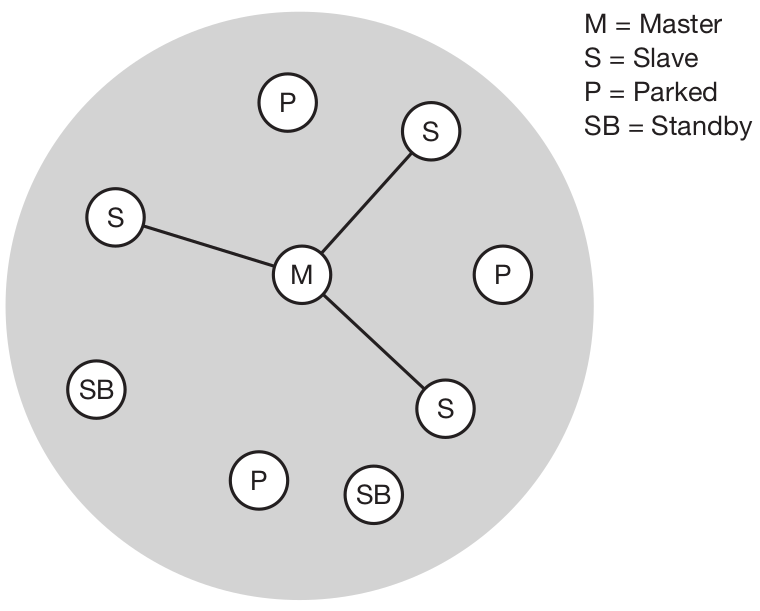
\includegraphics[width=0.8\textwidth]{bluetooth-piconet}
\caption{Simple Bluetooth piconet}\label{fig:bluetooth-piconet}
\end{figure}

\subsubsection{Scatternet}
All users within one piconet have the same hopping sequence and share the same 1 MHz channel. As more users join the piconet, the throughput per user drops quickly. This led to the idea of forming groups of piconets called \textbf{scatternet}. Only those units that really must exchange data share the same piconet, so that many piconets with overlapping coverage can exist simultaneously.


%%%%%%%%%%%%%%%%%%%%%%%%%%%%%%%%%%%%%%%%%%%%%%
%				
%				Figure
%
%%%%%%%%%%%%%%%%%%%%%%%%%%%%%%%%%%%%%%%%%%%%%%

\begin{figure}[h!]
\centering
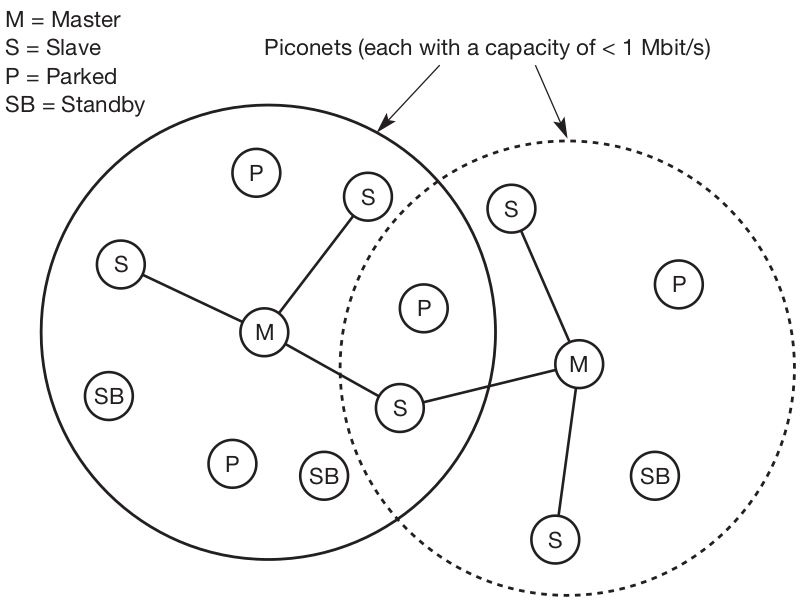
\includegraphics[width=0.8\textwidth]{bluetooth-scatternet}
\caption{Bluetooth scatternet}\label{fig:bluetooth-scatternet}
\end{figure}

In the example, 
\begin{multicols}{2}
	\begin{enumerate}
		\item the scatternet consists of two piconets, in which one device participates in two different piconets.
		\item Both piconets use a different hopping sequence, always determined by the master of the piconet. 
		\item In an average sense, all piconets can share the total of 80 MHz bandwidth available. 
		\item Adding more piconets leads to a graceful performance degradation of a single piconet because more and more
		collisions may occur. 
		\item A collision occurs if two or more piconets use the same carrier frequency at the same time. 
	\end{enumerate}
\end{multicols}



If a device wants to participate in more than one piconet:
\begin{multicols}{2}
\begin{itemize}
	\item It has to synchronize to the hopping sequence of the piconet it wants to take part in. 
	\item If a device acts as slave in one piconet, it simply starts to synchronize with the hopping sequence of the piconet it wants to join. 
	\item After synchronization, it acts as a slave in this piconet and no longer participates in its former piconet.
	\item Before leaving one piconet, a slave informs the current master that it will be unavailable for a certain amount of time. 
	\item The remaining devices in the piconet continue to communicate as usual.
\end{itemize}
\end{multicols}


A master can also leave its piconet and act as a slave in another piconet. As soon as a master leaves a piconet, all traffic within this piconet is suspended until the master returns.

Communication between different piconets takes place by devices jumping back and forth between theses nets. 

\subsection{Protocol Stack}
Bluetooth protocol stack can be thought of as a combination of multiple application specific stacks.

The Bluetooth protocol stack can be divided into a \textit{core specification}, which describes the protocols from physical layer to the data link control together with management functions, and \textbf{profile specifications}. The latter describes many protocols and functions needed to adapt the wireless Bluetooth technology to legacy and new applications.



%%%%%%%%%%%%%%%%%%%%%%%%%%%%%%%%%%%%%%%%%%%%%%
%				
%				Figure
%
%%%%%%%%%%%%%%%%%%%%%%%%%%%%%%%%%%%%%%%%%%%%%%

\begin{figure}[h]
\centering
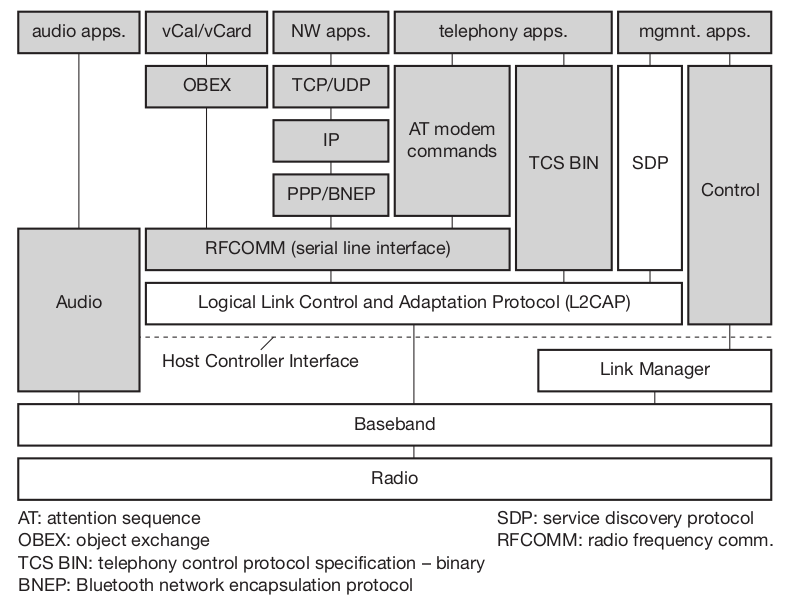
\includegraphics[width=0.8\textwidth]{bluetooth-protocol-stack}
\caption{Bluetooth protocol stack}\label{fig:bluetooth-protocol-stack}
\end{figure}

Bluetooth protocol stack (see figure \ref{fig:bluetooth-protocol-stack}) can be divided into different components according to their functions.

\subsubsection{Core Protocols}
The \textbf{core protocols} of Bluetooth comprise the following elements:
\begin{itemize}
\item \textbf{Radio}: Specification of the air interface, e.\ g.\ , frequencies, modulation, and transmit power.

\item \textbf{Baseband}: Description of basic connection establishment, packet formats, timing, and basic QoS parameters.

\item \textbf{Link manager protocol}: Link set-up and management between devices including security functions and parameter negotiation.

\item \textbf{Logical link control and adaptation protocol (L2CAP)}: Adaptation of higher layers to the baseband (connectionless and connection-oriented services).

\item \textbf{Service discovery protocol}: Device discovery in close proximity plus querying of service characteristics.
\end{itemize}

\subsubsection{Cable Replacement Protocol}
On top of L2CAP is the \textbf{cable replacement protocol} RFCOMM that emulates a serial line interface.
\begin{itemize}
	\item This allows for a simple replacement of serial line cables and enables many legacy applications and protocols to run over Bluetooth. 
	\item RFCOMM supports multiple serial ports over a single physical channel. 
	
\end{itemize}

\subsubsection{Telephony Control Protocol}
\begin{itemize}
	\item The \textbf{telephony control protocol specification - binary (TCS BIN)} describes a bit-oriented protocol that defines
	call control signaling for the establishment of voice and data calls between Bluetooth devices. 
	\item It also describes mobility and group management functions.
\end{itemize}

\subsubsection{Adopted Protocols}
Many protocols have been adopted in the Bluetooth standard. 
\begin{itemize}
	\item Classical Internet applications can still use the standard \textbf{TCP/IP} stack running over PPP or use the more efficient \textbf{Bluetooth network encapsulation protocol (BNEP)}. 
	\item Telephony applications can use the \textbf{AT modem commands} as if they were using a standard modem. 
	\item \textbf{Calendar and business card objects (vCalendar/vCard}) can be exchanged using the \textbf{object exchange protocol (OBEX)} as common with IrDA interfaces.
\end{itemize}



\subsubsection[Host Controller Interface]{Host Controller Interface (HCI)}
\begin{itemize}
	\item The HCI between the baseband and L2CAP provides a command interface to the baseband controller and link manager, and access to the hardware status and control registers. 
	\item The HCI can be seen as the hardware/software boundary.
\end{itemize}

\subsubsection{Audio}
\begin{itemize}
	\item A real difference to other protocol stacks is the support of audio. 
	\item Audio applications may directly use the baseband layer after encoding the audio signals.
\end{itemize}

	\begin{center}
\begin{framed}
	\begin{nepali}
		ब्लुटुथ प्राेटाेकल स्ट्याककाे सरल चित्र। माथि चित्रण गरिएकाे चित्रकाे साटाे याे बनाएपनि हुन्छ। (Simplified figure of Bluetooth protocol stack.)
	\end{nepali}
\end{framed}
\end{center}
\begin{figure*}[bph]
	\centering
	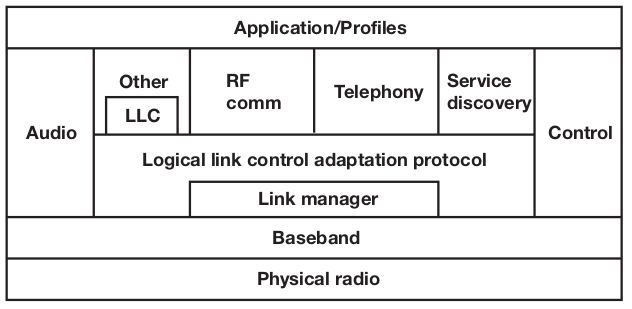
\includegraphics[width=0.7\textwidth]{bluetooth-protocol-stack-alternative}
%	\caption{Bluetooth protocol stack}
	\label{fig:bluetooth-protocol-stack-alternative}
\end{figure*}

\begin{figure}

\end{figure}

 % Chapter-2: Wireless LAN

\chapter[Global System For Mobile Communications]{Global System For Mobile Communications (GSM)}
\gls{gsm} is the most successful digital mobile telecommunication system in the world. It is used by billions of people around the world.

In the early 1980s, Europe had numerous coexisting analog mobile phone systems, which were often based on similar standards, but ran on slightly different carrier frequencies. To avoid this situation for a second generation fully digital system, the \textbf{groupe spéciale mobile (GSM)} was founded in 1982. This system was soon named the \textit{global system for mobile communications (GSM}), with the specification process lying in the hands of \gls{etsi}. 

The primary goal of \gls{gsm} was to provide a mobile phone system that allows users to roam throughout Europe and provides voice services compatible to \gls{isdn} and other \gls{pstn} systems.

\begin{itemize}
	\item \gls{gsm} is a typical second generation system, replacing the first generation analog systems. 
	\item \gls{gsm} has initially been deployed in Europe using 890–915 MHz for uplinks and 935–960 MHz for downlinks.
	\item There are multiple versions of \gls{gsm} system.
		\begin{itemize}
			\item \textbf{GSM 900}: GSM at 900 MHz.
			\item \textbf{Digital Cellular Service (DCS)} 1800: GSM at 1800 MHz.
			\item \textbf{Personal Communication Service (PCS) 19000}: GSM at 1900 MHz.	
		\end{itemize}
\end{itemize}


\section{Mobile Services}
\gls{gsm} permits the integration of different voice and data services and the interworking with existing networks. Services make a network interesting for customers. \gls{gsm} has defined three different categories of services: 
\begin{itemize}
	\item bearer services
	\item tele services and
	\item supplementary services
\end{itemize}

%%%%%%%%%%%%%%%%%%%%%%%%%%%%%%%%%%%%%%%%%%%%%%
%				
%				Figure
%
%%%%%%%%%%%%%%%%%%%%%%%%%%%%%%%%%%%%%%%%%%%%%%

%\begin{figure}[h]
%	\centering
%	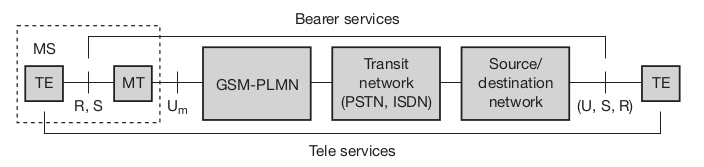
\includegraphics[width=0.8\textwidth]{bearer-and-tele-services}
%	\caption{Bearer and tele services reference model}\label{fig:bearer-and-tele-services}
%\end{figure}

%Figure \ref{fig:bearer-and-tele-services} shows a reference model for GSM services. A \textbf{mobile station MS} is
%connected to the \textbf{GSM public land mobile network (PLMN)} via the $ U_m $ interface. (GSM-PLMN is the infrastructure needed for the GSM network.) This
%network is connected to transit networks, e.g., \textbf{integrated services digital network (ISDN)} or traditional \textbf{public switched telephone network (PSTN)}. There
%might be an additional network, the source/destination network, before another
%\textbf{terminal TE} is connected. \textbf{Bearer services} now comprise all services that enable
%the transparent transmission of data between the interfaces to the network, i.e., $ S $
%in case of the mobile station, and a similar interface for the other terminal (e.g.,
%$ S_0 $ for ISDN terminals). Interfaces like $ U $, $ S $, and $ R $ in case of ISDN have not been
%defined for all networks, so it depends on the specific network which interface is
%used as a reference for the transparent transmission of data. In the classical GSM
%model, bearer services are connection-oriented and circuit- or packet-switched.
%These services only need the lower three layers of the ISO/OSI reference model.
%
%Within the mobile station MS, the \textbf{mobile termination (MT)} performs all
%network specific tasks (TDMA, FDMA, coding etc.) and offers an interface for
%data transmission (S) to the terminal TE which can then be network indepen-
%dent. Depending on the capabilities of TE, further interfaces may be needed,
%such as $ R $, according to the ISDN reference model. Tele services
%are application specific and may thus need all seven layers of the ISO/OSI refer-
%ence model. These services are specified end-to-end, i.e., from one terminal TE
%to another.

\subsection{Bearer Services}
Bearer services are telecommunication services that are used to transfer user data and control signals between two pieces of equipment.
Bearer services permit 
 \begin{itemize}
 	\item transparent and non-transparent, 
 	\item synchronous or asynchronous data transmission. 
 \end{itemize}

 
 \subsubsection*{Transparent Bearer Services}
 \begin{itemize}
 	\item Transparent bearer services only use the functions of the physical layer (layer 1) to transmit data. 
 	\item Data transmission has a constant delay and throughput if no transmission errors occur.
 	\item Transparent bearer services do not try to recover lost data.
 \end{itemize}

\subsubsection*{Non-transparent Bearer Services}
Non-transparent bearer services use protocols of layers two and three to implement error correction and flow control.

\subsection{Tele services}
\gls{gsm} mainly focuses on voice-oriented tele services. These comprise encrypted voice transmission, message services, and basic data communication with terminals as known from the \gls{pstn} or \gls{isdn}. 

%\subsection*{GSM Tele Services}

\subsubsection{Telephony}
The primary goal of GSM was the provision of high-quality digital voice transmission.

\subsubsection{Emergency Number}
This service is mandatory for all providers and free of charge. This connection also has the highest priority, possibly pre-empting other connections, and will automatically be set up with the closest emergency center.

\subsubsection{SMS}
\gls{sms} offers transmission of messages of up to 160 characters. It's successor is \gls{ems}.

\subsubsection{EMS}
\gls{ems} offers a \textit{larger message size} (e.\ g.\ , 760 characters), \textit{formatted text}, and the \textit{transmission of animated pictures}, \textit{small images} and \textit{ring tones} in a standardized way. 

\subsubsection{MMS}
EMS never really took off. \gls{mms} offers the transmission of \textit{larger pictures}, \textit{short video clips} etc. 

\subsubsection{Group 3 Fax}
Group 3 fax is a non-voice tele service. Fax data is transmitted as digital data over the analog telephone network using modems. 


\subsection{Supplementary services}
In addition to tele and bearer services, GSM providers can offer \textbf{supplementary services}. These services offer various enhancements for the standard telephony service. Typical services are:

\begin{multicols}{2}
	\begin{itemize}
		\item user identification
		\item call redirection
		\item closed user groups and 
		\item multi party communication
	\end{itemize}
\end{multicols}

Closed user groups allow, for example, a company-specific \gls{gsm} sub-network, to which only members of the group have access.

\section{System Architecture}
Figure \ref{fig:gsm-architecture} gives an overview of the \gls{gsm} system. A \gls{gsm} system consists of three subsystems:
%\begin{enumerate}
%	\item \textbf{the radio subsystem (RSS)}
%	\item \textbf{the network and switching subsystem (NSS)} and
%	\item \textbf{the operation subsystem (OSS)}
%\end{enumerate}
\begin{enumerate}
	\item \textit{\gls{rss}}
	\item \textit{\gls{nss}} and
	\item \textit{\gls{oss}}
\end{enumerate}

\begin{framed}
\begin{nepali}
\noindent नाेटः GSM Architecture with interface भनेमा Figure \ref{fig:gsm-architecture} मा देखाइएकाे सबै बनाउने।
\end{nepali}
\end{framed}


%%%%%%%%%%%%%%%%%%%%%%%%%%%%%
%							%
%		Chapters			%
%							%
%%%%%%%%%%%%%%%%%%%%%%%%%%%%%
\begin{figure}[hb!]
	\centering
	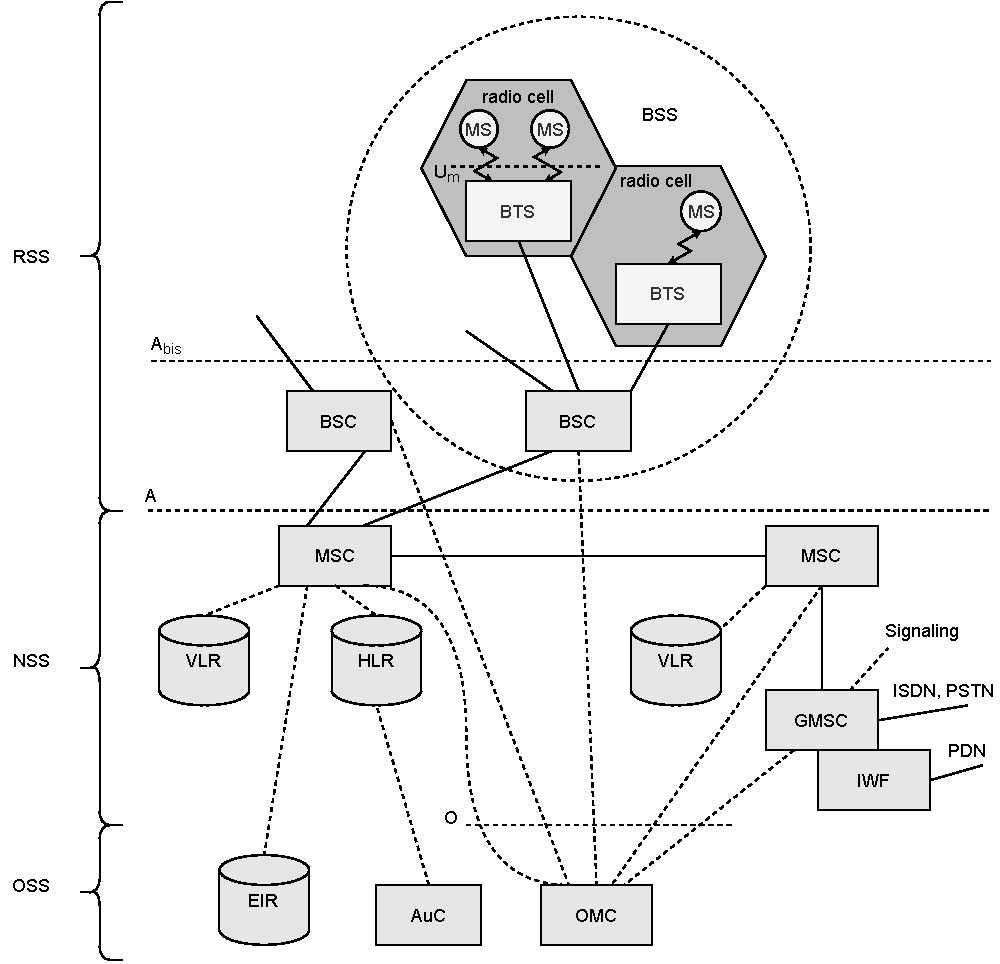
\includegraphics[width=0.8\textwidth]{gsm-architecture.pdf}
	\caption{Functional architecture of a GSM system}\label{fig:gsm-architecture}
\end{figure}

\subsection[Radio Subsystem]{Radio Subsystem (RSS)}
\begin{itemize}
	\item \gls{rss} comprises all radio specific entities, i.\ e.\,  \textit{\gls{ms}} and \textit{\gls{bss}}.
	\item Figure \ref{fig:gsm-architecture} shows the connection between the \gls{rss} and the \gls{nss} via the  \textbf{A interface} (solid lines) and the connection to the \gls{oss} via the \textbf{O interface} (dashed lines).
\end{itemize}


\subsubsection[BSS]{Base Station Subsystem (BSS)}
\begin{itemize}
	\item A \gls{gsm} network comprises many \gls{bss}s, each controlled by a \gls{bsc}. 
	\item The \gls{bss} performs all functions necessary to maintain: 
	\begin{itemize}
		\item radio connections to an \gls{ms}, 
		\item coding/decoding of voice, and 
		\item rate adaptation to/from the wireless network part.
	\end{itemize}
 \item Besides a \gls{bsc}, the \gls{bss} contains several BTSs.
\end{itemize}


\subsubsection[BTS]{Base Transceiver Station (BTS)}
\begin{itemize}
	\item A \gls{bts} comprises all radio equipment, i.\ e.\ , \textit{antennas}, \textit{signal processing}, \textit{amplifiers} necessary for radio transmission. 
	\item A \gls{bts}:
	\begin{itemize}
		\item can form a radio cell using sectorized antennas.
		\item is connected to \gls{ms} via the \( U_m \) {interface}, and 
		\item connected to the \gls{bsc} via the  \(A_{bis}\)  {interface}.
	\end{itemize}
\item The $ U_m $ interface contains all the mechanisms necessary for wireless transmission.
\item A \gls{gsm} cell can measure between some \(100 m\) and \(35 km\) depending on the environment. 
\end{itemize}


\paragraph*{Tasks of The \gls{bts} Within a \gls{bss}}
\begin{multicols}{2}
	\begin{itemize}
		\item Frequency hopping
		\item Channel coding and decoding
		\item Rate adaptation
		\item Encryption and decryption
		\item Paging
		\item Uplink signal measurement
	\end{itemize}
\end{multicols}


\subsubsection[BSC]{Base Station Controller (BSC)}
\begin{itemize}
	\item The \gls{bsc} basically manages the \gls{bts}s.
	\item It \textit{reserves radio frequencies}, \textit{handles the handover} from one \gls{bts} to another within the \gls{bss}, and \textit{performs paging} of the \gls{ms}. 
	\item The \gls{bsc} also \textit{multiplexes the radio channels} onto the fixed network connections at the \(A\) interface.
\end{itemize}


\paragraph*{Tasks of The \gls{bsc} Within a \gls{bss}}
\begin{multicols}{2}
	\begin{itemize}
		\item Management of radio channels
		\item Frequency hopping
		\item Management of terrestrial channels
		\item Mapping of terrestrial onto radio channels
		\item Encryption and decryption
		\item Paging
		\item Traffic measurement
		\item Authentication
		\item Location registry, location update
		\item Handover management
	\end{itemize}
\end{multicols}



\subsubsection[MS]{Mobile Station(MS)}
\begin{itemize}
	\item The \gls{ms} comprises all user equipment and software needed for communication with a \gls{gsm} network.
	\item An \gls{ms} consists of:
	\begin{itemize}
		\item user independent hardware and software and
		\item the \textit{\gls{sim}}, which stores all user-specific data that is relevant to \gls{gsm}\footnote{Many additional items can be stored on the mobile device. However, this is irrelevant to GSM.}. 
	\end{itemize}
\item An \gls{ms} can be identified via the \textit{\gls{imei}}.
\end{itemize}

 A user can personalize any \gls{ms} using his or her \gls{sim}. The \gls{sim} card contains many identifiers and tables, such as:
\begin{multicols}{2}
	\begin{itemize}
		\item card-type 
		\item serial number
		\item a list of subscribed services
		\item a \textit{\gls{pin}}
		\item a \textit{\gls{puk}}
		\item an authentication key $  K_i $ , and 
		\item the \textit{\gls{imsi}}
	\end{itemize} 
\end{multicols}

The \gls{pin} is used to unlock the \gls{ms}. Using the wrong \gls{pin} three times will lock the \gls{sim}. In such cases, the \gls{puk} is needed to unlock the \gls{sim}. The \gls{ms} stores dynamic information while logged onto the \gls{gsm} system, such as, e.\ g.\ , the cipher key $ K_c $ and the location information consisting of a \textit{\gls{tmsi}} and the \textit{\gls{lai}}.


\subsection[NSS]{Network and Switching Subsystem (NSS)}
\begin{itemize}
	\item The \textit{heart} of the GSM system is formed by the \textit{\gls{nss}}.
	\item The \gls{nss}: 
	\begin{itemize}
		\item connects the wireless network with standard public networks, 
		\item performs handovers between different \gls{bss}s, 
		\item comprises functions for worldwide localization of users and 
		\item supports charging, accounting, and roaming of users between different providers in different countries. 
	\end{itemize}
\end{itemize}

The \gls{nss} consists of the following switches and databases:

\subsubsection[MSC]{Mobile Services Switching Center (MSC)}
\begin{itemize}
	\item \gls{msc}s are high-performance digital ISDN switches. 
	\item They set up connections to other \gls{msc}s and to the \gls{bsc}s via the \(A\) interface, and form the fixed backbone network of a \gls{gsm} system. 
	\item Typically, an \gls{msc} manages several \gls{bsc}s in a geographical region. 
	\item A \gls{gmsc} has additional connections to other fixed networks, such as \gls{pstn} and \gls{isdn}. 
	\item Using additional \gls{iwf}, an \gls{msc} can also connect to \gls{pdn} such as \(X.25\). 
	\item An \gls{msc} handles all signaling needed for connection setup, connection release and handover of connections to other \gls{msc}s. 
	\item An \gls{msc} also performs all functions needed for supplementary services such as call forwarding, multi-party calls, etc.
\end{itemize}


\subsubsection[HLR]{Home Location Register (HLR)}
\begin{itemize}
	\item The \gls{hlr} is the most important database in a \gls{gsm} system as it stores all user-relevant information.
	\item This comprises static information, such as:
	\begin{itemize}
		\item \textit{\gls{msisdn}},
		\item subscribed services (e.\ g.\ , call forwarding, roaming restrictions, GPRS), and
		\item \textit{\gls{imsi}}
	\end{itemize}
\item  Dynamic information is also needed:
	\begin{itemize}
	\item \textit{\gls{la}} of the \gls{ms},
	\item \textit{\gls{msrn}},
	\item current \gls{vlr} and \gls{msc}.
\end{itemize}

\item As soon as an \gls{ms} leaves its current \gls{la}, the information in the \gls{hlr} is updated.
\item All these user-specific information elements only exist once for each user in a single \gls{hlr}.
\item Responsible for charging and accounting.
\item \gls{hlr} contains highly specialized databases to perform various specialized tasks such as answering requests within certain time-bounds.
\end{itemize}
 
\subsubsection[VLR]{Visitor Location Register (VLR)}
\begin{itemize}
	\item The \gls{vlr} associated to each \gls{msc} is a dynamic database. 
	\item \gls{vlr} stores all important information needed for the \gls{ms} users currently in the \gls{la} that is associated to the \gls{msc}. 
	\item If a new \gls{ms} comes into an \gls{la} the \gls{vlr} is responsible for, it copies all relevant information for this user from the \gls{hlr}. 
	\item This hierarchy of \gls{vlr} and \gls{hlr} avoids frequent \gls{hlr} updates and long-distance signaling of user information.
\end{itemize}


\subsection[OSS]{Operation Subsystem (OSS)}
The third part of a \gls{gsm} system, the \gls{oss} contains the necessary functions for network operation and maintenance. The following entities have been defined:

\subsubsection[OMC]{Operation and Maintenance Center (OMC)}
 The \gls{omc} monitors and controls all other network entities via the \(O\) interface. Typical \gls{omc} management functions are:
\begin{itemize}
	\item traffic monitoring
	\item status reports of network entities
	\item subscriber and security management
	\item accounting and billing
\end{itemize}

\subsubsection[AuC]{Authentication Center (AuC)}
\begin{itemize}
	\item The \gls{auc} contains the algorithms for authentication as well as the keys for encryption and 
	\item Generates the values needed for user authentication in the \gls{hlr}. 
	\item The \gls{auc} may be situated in a special protected part of the \gls{hlr}.
\end{itemize}

\subsubsection[EIR]{Equipment Identity Register (EIR)}
\begin{itemize}
	\item The \gls{eir} is a database for all \gls{imei}s.
	\item The \gls{eir} has a \textit{blacklist} of stolen (or locked) devices.
	\item The \gls{eir} also contains a list of valid \gls{imei}s (\textit{white list}), and a list of malfunctioning devices (\textit{gray list}).
\end{itemize}
 
\section{Protocols}
\gls{gsm} architecture is a layered model that is designed to allow communications between two different systems. The lower layers assure the services of the upper-layer protocols. Each layer passes suitable notifications to ensure the transmitted data has been formatted, transmitted, and received accurately.

Figure \ref{fig:gsm-protocol-architecture} shows the protocol architecture of \gls{gsm} with signaling protocols, interfaces, as well as the entities already shown in Figure \ref{fig:gsm-architecture}. 

\begin{figure}[hb!]
	\centering
	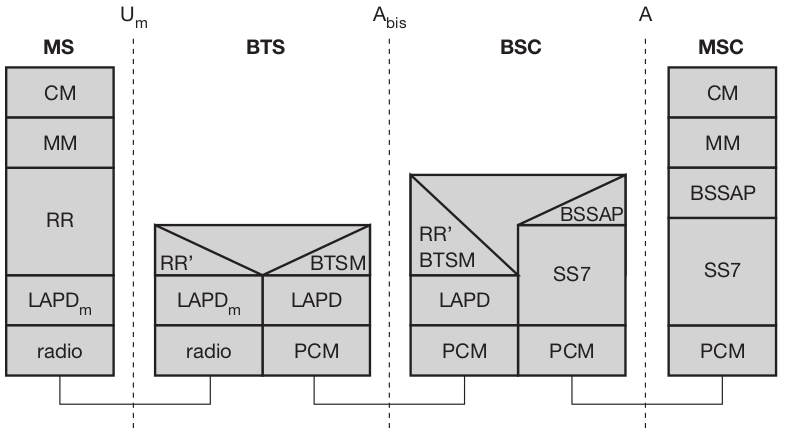
\includegraphics[width=0.8\textwidth]{gsm-protocol-architecture}
	\caption[GSM Protocol architecture.]{Protocol architecture for signaling}
	\label{fig:gsm-protocol-architecture}
\end{figure}



\subsection{MS Protocols}

\subsubsection{Layer 1: Physical Layer}
Layer 1, the \textit{physical layer}, handles all \textit{radio specific} functions.
\begin{itemize}
	\item channel coding
	\item error detection/correction
\end{itemize}

%\subsection*{PCM}
%Data transmission at the physical layer typically uses pulse code modulation (PCM) systems.


\subsubsection{Layer 2: Data Link Layer}
\begin{itemize}
	\item In layer 2, at the \(U_m\) interface, \(\mathbf{LAPD_m}\) has been defined for the purpose of signaling between entities in a \gls{gsm} network.
	\item \(\mathbf{LAPD_m}\) has been derived from link access procedure for the D-channel (LAPD) in ISDN systems, which is a version of HDLC.
	\item \(\mathbf{LAPD_m}\) is a lightweight LAPD because it does not need synchronization flags or checksumming for error detection.
\end{itemize}

%\subsubsection*{Signaling System No. 7 (SS7)} 
%SS7 is used for signaling between an MSC and a BSC. This protocol also transfers all management information between MSCs, HLR, VLRs, AuC, EIR, and OMC. 


\subsubsection{Layer 3: Network Layer}
The network layer in GSM, layer three, comprises several sublayers as shown in Figure \ref{fig:gsm-protocol-architecture}.

\begin{enumerate}
	\item Radio Resource Management (RR)
	\item Mobility Management (MM)
	\item Connection Management (CM)
\end{enumerate}

\subsection{MS to BTS Protocols}

\subsubsection*{RR}
The lowest sublayer is the radio resource management (RR). The main tasks of RR are:
\begin{itemize}
	\item \textit{setup}, \textit{maintenance}, and \textit{release of radio channels}.
	\item RR also directly accesses the physical layer for radio information and offers a reliable connection to the next higher layer.
\end{itemize}

\subsubsection*{MM}
The MM layer is stacked above the RR layer.
 \begin{itemize}
 	\item Mobility management (MM) contains functions for \textit{registration}, \textit{authentication}, \textit{identification}, \textit{location updating}, and the \textit{provision of a TMSI} that replaces the IMSI.
 	\begin{itemize}
 		\item TMSI hides the real identity of an MS user over the air interface.
 		\item TMSI is valid only in the current location area of a VLR.
 	\end{itemize}
 	\item MM offers a reliable connection to the next higher layer.
 \end{itemize}

\subsubsection*{CM}
The CM layer is the topmost layer of the GSM protocol stack. The call management (CM) layer contains three entities: 
\begin{multicols}{2}
	\begin{enumerate}
		\item call control (CC), 
		\item short message service (SMS), and 
		\item supplementary service (SS).
	\end{enumerate}
\end{multicols}

\paragraph*{SMS} allows for message transfer.

\paragraph*{CC} provides a point-to-point connection between two terminals and is used by higher layers for call establishment, call clearing and change of call parameters.

%\subsubsection*{BSSAP}
%An MSC can also control a BSS via a BSS application part (BSSAP).\\
%
%\noindent Additional protocols are used at the \(A_bis\) and \(A\) interfaces. LAPD is used for layer 2 at \(A_bis\), BTSM for BTS management.

\subsection{BSC Protocols}
\begin{itemize}
	\item The BSC uses a different set of protocols after receiving the data from the BTS. 
	\item The \(A_{bis}\) interface is used between the BTS and BSC.
	\item At this level, the radio resources at the lower portion of Layer 3 are changed from the RR to the Base Transceiver Station Management (BTSM). 
	\item The BTS management layer is a relay function at the BTS to the BSC.
\end{itemize}

The RR protocols are responsible for the allocation and reallocation of traffic channels between the MS and the BTS.

To transit from the BSC to the MSC, the BSS mobile application part or the direct application part is used, and SS7 protocols is applied by the relay.

\subsection{MSC Protocols}

\begin{itemize}
	\item At the MSC, starting from the BSC, the information is mapped across the \(A\) interface to the MTP Layers 1 through 3.
	\item Here, Base Station System Management Application Part (BSS MAP) is said to be the equivalent set of radio resources.
	\item The relay process is finished by the layers that are stacked on top of Layer 3 protocols, they are BSS MAP/DTAP, MM, and CM.
	\item This completes the relay process.
	\item To find and connect to the users across the network, MSCs interact using the control-signaling network.
\end{itemize}

%Each GSM MS user is given a HLR that in turn comprises the user’s location and subscribed services. VLR is a separate register that is used to track the location of a user. When the users move out of the HLR covered area, the VLR is notified by the MS to find the location of the user. The VLR in turn, with the help of the control network, signals the HLR of the MS’s new location. With the help of location information contained in the user’s HLR, the MT calls can be routed to the user.

\section{Localization and Calling}
One fundamental feature of the GSM system is the automatic, worldwide localization of users. The system always knows where a user currently is, and the same phone number is valid worldwide. To provide this service, GSM performs periodic location updates even if a user does not use the mobile station (provided that the MS is still logged into the GSM network and is not completely switched off). 

The HLR always contains information about the current location, and the VLR currently responsible for the MS informs the HLR about location changes. As soon as an MS moves into the range of a new VLR (a new location area), the HLR sends all user data needed to the new VLR. \textbf{Changing VLRs with uninterrupted availability of all services is also called roaming}. Roaming can take place within the network of one provider, between two providers in one country, but also between different providers in different countries (international roaming).

\subsection{Localization}
To locate an MS and to address the MS, several numbers are needed:

\subsubsection{MSISDN}
MSISDN is the phone number of a GSM user. It follows the standard for addresses as it is also used in fixed ISDN networks. This number
consists of the:
\begin{itemize}
	\item \textbf{country code} (CC) (e.\ g.\, \texttt{+977 024-123456} with 977 for Nepal)
	\item the \textbf{national destination code (NDC)} (i.\ e.\ , the address of the network provider), and 
	\item the \textbf{subscriber number (SN)}.
\end{itemize}

\subsubsection{IMSI}
 \begin{itemize}
 	\item GSM uses the IMSI for internal unique identification of a subscriber.
 	\item IMSI consists of:
 		\begin{itemize}
 			\item a \textbf{mobile country code (MCC)} (e.\ g.\ , 429 for Nepal), 
 			\item the \textbf{mobile network code (MNC)} (i.\ e.\ , the code of the network provider. e.\ g.\ , 01 for Nepal Telecom, 02 for Ncell), and finally
 			\item the \textbf{mobile subscriber identification number (MSIN)}.
 		\end{itemize}
 \end{itemize}  

\subsubsection{TMSI}

\begin{itemize}
	\item TMSI hides the IMSI to prevent leaking identity of the user signaling over the air interface. 
	\item GSM uses the 4 byte TMSI for local subscriber identification.
	\item TMSI is selected by the current VLR.
	\item TMSI is only valid temporarily and within the location area of the VLR.
	\item VLR may change the TMSI periodically.
\end{itemize}

\subsubsection[MSRN]{Mobile Station Roaming Number (MSRN)}
\begin{itemize}
	\item MSRN is slo a temporary address that hides the identity and location of a subscriber.
	\item The VLR generates this address on request from the MSC, and the address is also stored in the HLR.
	\item MSRN contains:
	\begin{itemize}
		\item the current \textbf{visitor country code (VCC)}, 
		\item the \textbf{visitor national destination code (VNDC)}, 
		\item the identification of the current MSC together with the subscriber number.
	\end{itemize}
\item The MSRN helps the HLR to find a subscriber for an incoming call.
\end{itemize}

\noindent All these numbers are needed to find a subscriber and to maintain the connection with a mobile station. The interesting case is the \textbf{mobile terminated call (MTC)}.

\subsection{Calling}
There are two approaches to call setup:
\begin{itemize}
	\item \textit{Mobile originated call (MOC)}: Mobile subscriber initiates the call.
	\item \textit{Mobile terminated call (MTC)}: Subscriber Receives the call.
\end{itemize}
\subsubsection{MTC}
MTC is a situation in which a station calls a mobile station (the calling station could be outside the GSM network or another mobile station). Figure \ref{fig:mtc-mobile-terminated-call} shows the basic steps needed to connect the calling station with the mobile user. 

%%%%%%%%%%%%%%%%%%%%%%%%%%%%%
%							%
%		FIGURE				%
%							%
%%%%%%%%%%%%%%%%%%%%%%%%%%%%%
\begin{figure}[hb!]
	\centering
	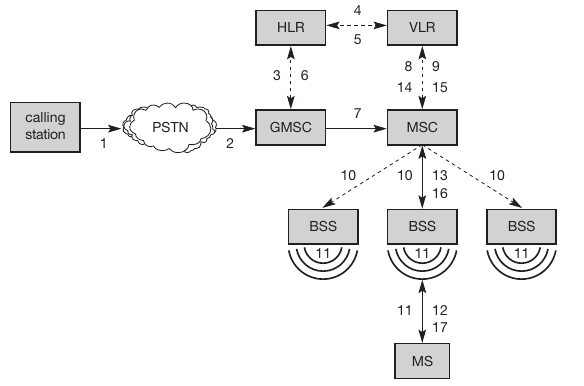
\includegraphics[width=0.8\textwidth]{mtc-mobile-terminated-call}
	\caption{Mobile terminated call (MTC)}
	\label{fig:mtc-mobile-terminated-call}
\end{figure}

Following are the steps involved during MTC:
\begin{steps}
\item A user dials the phone number of a GSM subscriber. 
\item The PSTN forwards the call setup to the GMSC.
\item The GMSC identifies the HLR for the subscriber and signals the call setup to the HLR.
\item The HLR now checks whether the number exists and whether the user has subscribed to the requested services, and requests an MSRN from the current VLR.
\item HLR Receives an MSRN from the VLR.
\item The HLR can determine the MSC responsible for the MS and forwards this information to the GMSC.
\item The GMSC can now forward the call setup request to the MSC indicated.
		\subitem From this point on, the MSC is responsible for all further steps.
\item Requests the current status of the MS from the VLR.
\item Receives the status of the MS.
\item MSC initiates paging in all cells it is responsible for, if the MS is available.
\item The BTSs of all BSSs transmit this paging signal to the MS.
\item MS answers to the BSS.
\item BSS answers to the MSC.
\item The VLR has to perform security checks (set up encryption etc.).
\item The VLR then signals to the MSC to set up a connection.
\item MSC then signals BSS to set up a connection.
\item BSS then signals MS to set up a connection.
\end{steps}




\subsubsection{MOC}
It is much simpler to perform a MOC compared to a MTC (see Figure \ref{fig:moc-mobile-originated-call}). 

Following steps are involved during MOC:

\begin{steps}
	\item The MS transmits a request for a new connection.
	\item The BSS forwards this request to the MSC.
	\item The MSC request VLR to checks if this user is allowed to set up a call with the requested service.\label{itm:Step-3}
	\item VLR confirms request made in \ref{itm:Step-3} and signals to the MSC.
	\item MSC request GMSC for the availability of resources through GSM network.
	\item GMSC then request PSTN for resources.
	\item PSTN responds to GMSC.
	\item GMSC responds back to MSC.
	\item MSC sets up connection with BSS.
	\item BSS and MSC then sets up connection between MS and the fixed network. 
\end{steps}

%%%%%%%%%%%%%%%%%%%%%%%%%%%%%
%							%
%		FIGURE				%
%							%
%%%%%%%%%%%%%%%%%%%%%%%%%%%%%
\begin{figure}[ht!]
	\centering
	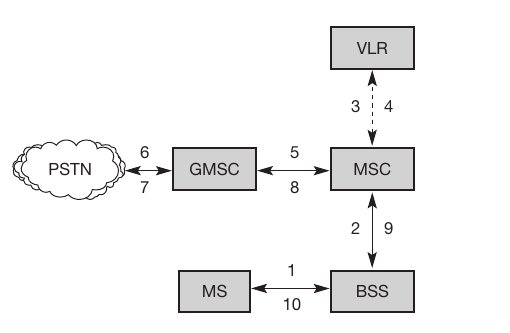
\includegraphics[width=0.8\textwidth]{moc-mobile-originated-call}
	\caption{Mobile originated call (MOC)}\label{fig:moc-mobile-originated-call}
\end{figure}

\begin{framed}
\subsubsection*{\textnp{MOC लाई बुँदागत रुपमा नलेखेर सङ्‍क्षेपमा यस प्रकारले पनि लेख्न सकिन्छ}}
It is much simpler to perform a mobile originated call (MOC) compared to a MTC. The MS transmits a request for a new connection (1), the BSS forwards this request to the MSC (2). The MSC then checks if this user is allowed to set up a call with the requested service (3 and 4) and checks the availability of resources through the GSM network and into the PSTN. If all resources are available, the MSC sets up a connection between the MS and the fixed network.
\end{framed}

\section{Handover}

Cellular systems require \textit{handover} procedures, as single cells do not cover the whole service area, but, e.\ g.\ , only up to 35 km around each antenna on the countryside and some hundred meters in cities. The smaller the cell size and the faster the movement of a mobile station through the cells (up to \(250 km/h\) for GSM), the more handovers of ongoing calls are required. However, a handover should not cause a cut-off, also called call drop. GSM aims at maximum handover duration of \(60 ms\).

\subsection{Basic Reasons For Handover}
There are two basic reasons for a handover:


\subsubsection[Out of Range]{MS moves out of the range of a BTS}
\begin{itemize}
	\item The mobile station moves out of the range of a BTS or a certain antenna of a BTS respectively.
	\item The received \textit{signal level} decreases continuously until it falls below the minimal requirements for communication.
	\item \textit{The error rate} may grow due to interference, the distance to the BTS may be too high
	\item All these effects may diminish the \textit{quality of the radio link} and make radio transmission impossible in the near future.
\end{itemize}
 


\subsubsection[High Traffic]{Too high traffic in one cell}

\begin{itemize}
	\item The wired infrastructure (MSC, BSC) may decide that the \textit{traffic in one cell is too high} and shift some MS to other cells with a lower load (if possible).
	\item Handover may be due to \textit{load balancing}.
\end{itemize}

\subsection{Handover Scenarios}
Figure \ref{fig:gsm-handover} shows four possible handover scenarios in GSM:

\begin{itemize}
	\item \textit{Intra-cell handover}.	
	\item \textit{Inter-cell, intra-BSC handover}
	\item \textit{Inter-BSC, intra-MSC handover}:
	\item \textit{Inter MSC handover}
\end{itemize}

%%%%%%%%%%%%%%%%%%%%%%%%%%%%%
%							%
%		FIGURE				%
%							%
%%%%%%%%%%%%%%%%%%%%%%%%%%%%%
\begin{figure}[ht!]
	\vspace*{0.2cm}
	\centering
	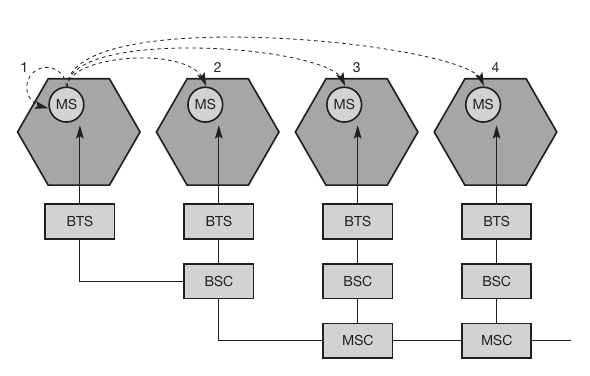
\includegraphics[width=0.8\textwidth]{gsm-handover}
	\caption{Types of handover in GSM}\label{fig:gsm-handover}
\end{figure}

\subsubsection[Intra-cell Handover]{Scenario 1: Intra-cell Handover}
\begin{itemize}
	\item Within a cell, narrow-band interference could make transmission at a certain frequency impossible. 
	\item The BSC could then decide to change the carrier frequency.
\end{itemize}

\subsubsection[Inter-cell, Intra-BSC Handover]{Scenario 2: Inter-cell, Intra-BSC Handover}
\begin{itemize}
	\item This is a typical handover scenario. 
	\item The mobile station moves from one cell to another, but stays within the control of the same BSC. 
	\item The BSC then performs a handover, assigns a new radio channel in the new cell and releases the old one.
\end{itemize}


\subsubsection[Inter-BSC, Intra-MSC Handover]{Scenario 3: Inter-BSC, Intra-MSC Handover}
\begin{itemize}
	\item As a BSC only controls a limited number of cells; GSM also has to perform handovers between cells controlled by different BSCs.
	\item This handover then has to be controlled by the MSC.
\end{itemize}

\subsubsection[Inter MSC handover]{Scenario 4: Inter MSC handover}
\begin{itemize}
	\item A handover could be required between two cells belonging to different MSCs. 
	\item Now both MSCs perform the handover together.
\end{itemize}


\noindent Figure \ref{fig:intra-msc-handover} shows the typical signal flow during an inter-BSC, intra-MSC handover. 

\begin{itemize}
	\item The MS sends its periodic measurements reports, the $ BTS_{old} $ forwards these reports to the $ BSC_{old} $ together with its own measurements. 
	\item Based on these values and, the $ BSC_{old} $ may decide to perform a handover and sends the message \verb*|HO_required| to the MSC. 
	\item The task of the MSC then comprises the request of the resources needed for the handover from the new BSC, $ BSC_{new} $. 
	\item This BSC checks if enough resources  are available and activates a physical channel at the $ BTS_{new} $ to prepare for the arrival of the MS.
	\item The $ BTS_{new} $ acknowledges the successful channel activation, $ BSC_{new} $ acknowledges the handover request. 
	\item The MSC then issues a handover command that is forwarded to the MS. 
	\item The MS now breaks its old radio link and accesses the new BTS. 
	\item The next steps include the establishment of the link (this includes layer two link establishment and handover complete messages from the MS). 
	\item Basically, the MS has then finished the handover, but it is important to release the resources at the old BSC and BTS and to signal the successful handover using the handover and clear complete messages as shown.
\end{itemize}



%%%%%%%%%%%%%%%%%%%%%%%%%%%%%
%							%
%		FIGURE				%
%							%
%%%%%%%%%%%%%%%%%%%%%%%%%%%%%

\begin{figure}[ht!]
	\centering
	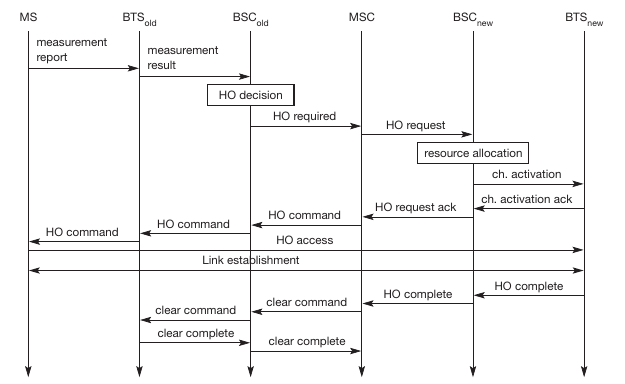
\includegraphics[width=0.8\textwidth]{intra-msc-handover}
	\caption{Intra-MSC handover}\label{fig:intra-msc-handover}
\end{figure}



\section{Security}
GSM offers several security services using confidential information stored in the AuC and in the individual SIM (which is plugged into an arbitrary MS). The SIM stores personal, secret data and is protected with a PIN against unauthorized use. (For example, the secret key \(K_i\) used for authentication and encryption procedures is stored in the SIM.) 

\subsection{GSM Security Services}
The security services offered by GSM are:
\begin{itemize}
	\item \textit{Access control and authentication}
	\item \textit{Confidentiality}
	\item \textit{Anonymity}
\end{itemize}

\subsubsection{Access Control and Authentication}
\begin{itemize}
	\item The first step includes the authentication of a valid user for the SIM. The user needs a secret PIN to access the SIM.
	\item The next step is the subscriber authentication. 
	\item This step is based on a challenge-response scheme as presented in Section \ref{sec:challenge-response}.
\end{itemize}

\subsubsection{Confidentiality}
\begin{itemize}
	\item All user-related data is encrypted. 
	\item After authentication, BTS and MS apply encryption to voice, data, and signaling as shown in Section \ref{sec:encryption}. 
	\item This confidentiality exists only between MS and BTS, but it does not exist end-to-end or within the whole fixed GSM/telephone network.
\end{itemize}


\subsubsection{Anonymity}
\begin{itemize}
	\item To provide user anonymity, all data is encrypted before transmission, and user identifiers are not used over the air.
	\item Instead, GSM transmits a temporary identifier (TMSI), which is newly assigned by the VLR after each location update.
	\item Additionally, the VLR can change the TMSI at any time.
\end{itemize}

\noindent Three algorithms have been specified to provide security services in GSM:
\begin{itemize}
	\item Algorithm $ A3 $ is used for \textit{authentication},
	\item $ A5 $ for \textit{encryption}, and
	\item $ A8 $ for the \textit{generation of a cipher key}.
\end{itemize}

\noindent In the GSM standard only algorithm $ A5 $ was publicly available, whereas $ A3 $ and $ A8 $ were secret, but standardized with open interfaces. Both $ A3 $ and $ A8 $ are no longer secret, but were published on the internet in 1998. 

Algorithms $ A3 $ and $ A8 $ (or their replacements) are located on the SIM and in the AuC and can be proprietary. Only $ A5 $ which is implemented in the devices has to be identical for all providers.

\subsection{Authentication}\label{sec:challenge-response}
Before a subscriber can use any service from the GSM network, he or she must be authenticated. Authentication is based on the SIM, which stores the: 
%\begin{multicols}{2}
\begin{enumerate}
	\item \textbf{individual authentication key} $ K_i $, 
	\item \textbf{user identification IMSI}, and 
	\item algorithm used for authentication \textbf{A3}. 
\end{enumerate}
%\end{multicols}



\noindent Authentication uses a challenge-response method:
\begin{steps}
	\item The access control AC generates a random number \textbf{RAND} as challenge, and 
	\item the SIM within the MS answers with \textbf{SRES} (signed response) as response (see Figure \ref{fig:subscriber-auth}). 
	\item The AuC performs the basic generation of random values $ RAND $, signed responses $ SRES $, and cipher keys $ K_c $ for each IMSI, and then forwards this information to the HLR. 
	\item The current VLR requests the appropriate values for $ RAND $, $ SRES $, and $ K_c $ from the HLR.
	\item The VLR sends the random value $ RAND $ to the SIM. 
	\item Both sides, network and subscriber module, perform the same operation with $ RAND $ and the key $ K_i $, called $ A3 $. 
	\item The MS sends back the $ SRES $ generated by the SIM; the VLR can now compare both values. 
	\item If they are the same, the VLR accepts the subscriber, otherwise the subscriber is rejected.
\end{steps}



%%%%%%%%%%%%%%%%%%%%%%%%%%%%%
%							%
%		FIGURE				%
%							%
%%%%%%%%%%%%%%%%%%%%%%%%%%%%%

\begin{figure}[ht!]
	\vspace*{0.2cm}
	\centering
	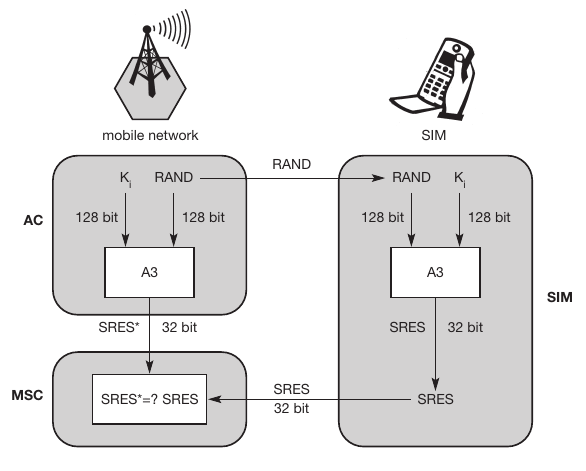
\includegraphics[width=0.8\textwidth]{subscriber-auth}
	\caption{Subscriber authentication}\label{fig:subscriber-auth}
\end{figure}


\subsection{Encryption}\label{sec:encryption}
To ensure privacy, all messages containing user-related information are encrypted in GSM over the air interface. 

\begin{itemize}
	\item After authentication, MS and BSS can start using encryption by applying the cipher key $ K_c $. 
	\item $ K_c $ is generated using the individual key $ K_i $ and a random value by applying the algorithm $ A8 $. 
	\item SIM in the MS and the network both calculate the same $ K_c $ based on the random value RAND. 
	\item The key $ K_c $ itself is not transmitted over the air interface.
\end{itemize}
%%%%%%%%%%%%%%%%%%%%%%%%%%%%%
%							%
%		FIGURE				%
%							%
%%%%%%%%%%%%%%%%%%%%%%%%%%%%%

\begin{figure}[ht!]
	\centering
	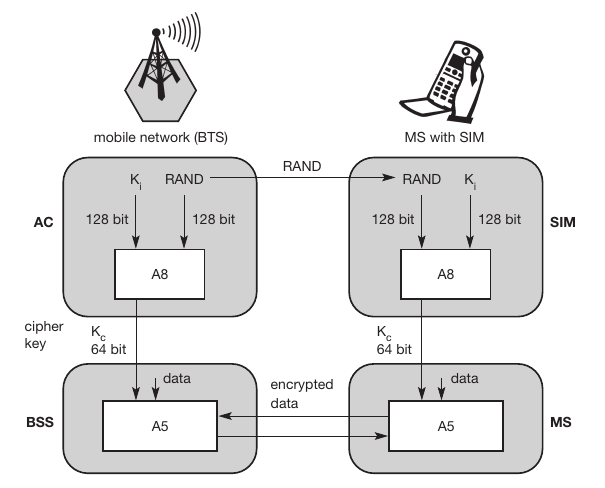
\includegraphics[width=0.8\textwidth]{data-encryption}
	\caption{Data encryption}\label{fig:data-encryption}
\end{figure}

MS and BTS can now encrypt and decrypt data using the algorithm A5 and the cipher key $ K_c $. As Figure \ref{fig:data-encryption} shows, $ K_c $ should be a 64 bit key — which is not very strong, but is at least a good protection against simple eavesdropping.


\newpage
\section{GPRS}
The general packet radio service (GPRS) provides packet mode transfer for applications that exhibit traffic patterns such as frequent transmission of small volumes (e.\ g.\ , typical web requests) or infrequent transmissions of small or medium volumes (e.\ g.\ , typical
web responses) according to the requirement specification. 

The key element of GPRS technology is that it uses packet switched data rather than circuit switched data, and this technique makes much more efficient use of the available capacity. The data is split into packets and tags inserted into the packet to provide the destination address. Packets from several sources can then be transmitted over the link.

\subsection*{Goal}
The provision of a more efficient and, thus, cheaper packet transfer service for typical internet applications that usually rely solely on packet transfer. 

\subsection*{Benefit}
The main benefit for users of GPRS is the `always on’ characteristic — no connection has to be set up prior to data transfer.

\subsection*{Motivation for Development} 
GPRS was driven by the tremendous success of the packet-oriented internet, and by the new traffic models and applications.


\subsection{GPRS System Architecture}
%The GPRS architecture introduces two new network elements, which are called \textbf{GPRS support nodes (GSN)} and \textbf{serving GPRS support node (SGSN)} 

\subsubsection[GSN]{GPRS Support Node (GSN)}
\textbf{GPRS support nodes (GSN)} and are in fact routers. All GSNs are integrated into the standard GSM architecture, and many new interfaces have been defined (see Figure \ref{fig:gprs-arch}). 

\subsubsection[GGSN]{Gateway GPRS Support Node (GGSN)}
The \textbf{gateway GPRS support node (GGSN)} is the interworking unit between the GPRS network and external \textbf{packet data networks (PDN)}. This node
\begin{itemize}
	\item contains routing information for GPRS users, 
	\item performs address conversion, and 
	\item tunnels data to a user via encapsulation.
\end{itemize}
 The GGSN is connected to external networks (e.\ g.\ , IP or X.25) via the $ G_i $ interface and transfers packets to the SGSN via an IP-based GPRS backbone network ($ G_n $ interface).

\subsubsection[SGSN]{Serving GPRS Support Node}
The \textbf{serving GPRS support node (SGSN)} which supports the MS via the $ G_b $ interface. The SGSN, for example, 
\begin{itemize}
	\item requests user addresses from the \textbf{GPRS register (GR)}, 
	\item keeps track of the individual MSs' location, is responsible for collecting billing information (e.\ g.\ , counting bytes), and \item performs several security functions such as access control.
\end{itemize}


 \noindent The SGSN is connected to a BSC via frame relay and is basically on the same hierarchy level as an MSC. The GR, which is typically a part of the HLR, stores all GPRS-relevant data. GGSNs and SGSNs can be compared with home and foreign agents, respectively, in a mobile IP network.
 
%%%%%%%%%%%%%%%%%%%%%%%%%%%%%%%%%%%%%%%%%%%%%
%											%
%				Figure						%
%											%
%%%%%%%%%%%%%%%%%%%%%%%%%%%%%%%%%%%%%%%%%%%%%
\begin{figure}[H]
	\centering
	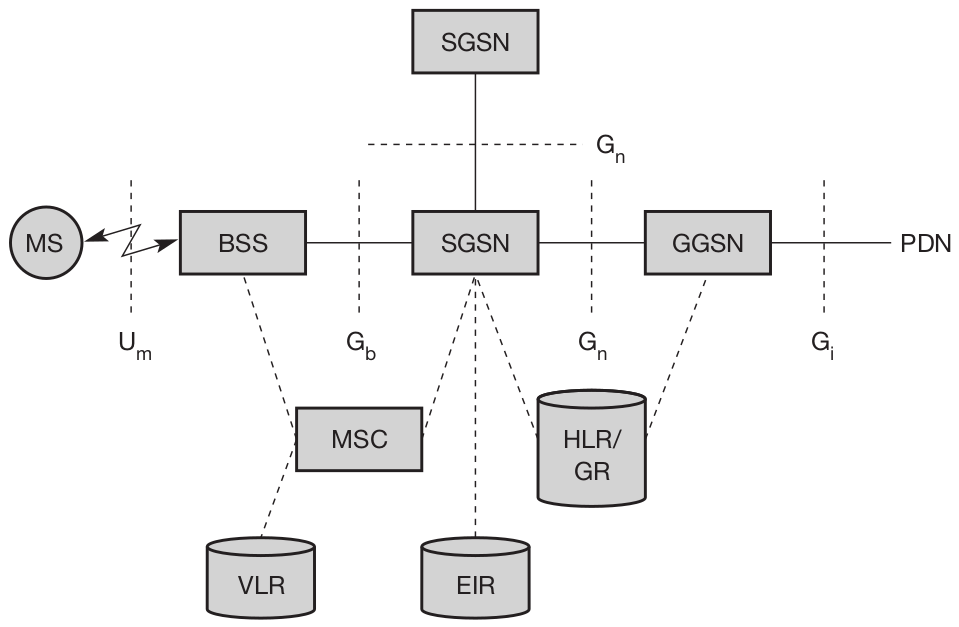
\includegraphics[width=0.8\textwidth]{gprs-arch}
	\caption{GPRS architecture reference model}\label{fig:gprs-arch}
\end{figure}
%-----------------------FIGURE END------------------------
As shown in Figure \ref{fig:gprs-arch}, packet data is transmitted from a PDN, via the GGSN and SGSN directly to the BSS and finally to the MS. The MSC, which is responsible for data transport in the traditional circuit-switched GSM, is only used for signaling in the GPRS scenario.


Before sending any data over the GPRS network, 
\begin{itemize}
	\item An MS must attach to it, following the procedures of the \textbf{mobility management}. 
	\item The attachment procedure includes assigning a temporal identifier, called a \textbf{temporary logical link identity (TLLI)}, and a \textbf{ciphering key sequence number (CKSN)} for data encryption. 
	\item For each MS, a \textbf{GPRS context} is set up and stored in the MS and in the corresponding SGSN. This context comprises:
	\begin{itemize}
		\item the status of the MS (which can be ready, idle, or standby), 
		\item the CKSN, 
		\item a flag indicating if compression is used, and 
		\item routing data (TLLI, the routing area RA, a cell identifier, and a packet data channel, PDCH, identifier)
	\end{itemize}
 \item Besides attaching and detaching, mobility management also comprises functions for:
 	\begin{itemize}
 		\item authentication, 
 		\item location management, and 
 		\item ciphering.
 	\end{itemize} 
 \item In \textbf{idle} mode an MS is not reachable and all context is deleted.
 \item In the \textbf{standby} state only movement across routing areas is updated to the SGSN but not changes of the cell.
\end{itemize}

Permanent updating would waste battery power, no updating would require system-wide paging. The update procedure in standby mode is a compromise. Only in the \textbf{ready} state every movement of the MS is indicated to the SGSN.



\section{UMTS}
The Universal Mobile Telecommunications System (UMTS) is a third generation mobile cellular system for networks based on the GSM standard. Developed and maintained by the 3GPP ($ 3^{rd} $ Generation Partnership Project), UMTS is a component of the Standard International Union all IMT-2000 telecommunications and compares it with the standard set for CDMA2000 networks based on competition cdmaOne technology. UMTS uses wideband code division multiple access (W-CDMA) radio access technology to provide greater spectral efficiency and bandwidth mobile network operators.

\subsection{UMTS System Architecture}

Figure \ref{fig:umts-components} shows the very simplified UMTS reference architecture.

\begin{itemize}
	\item The \textbf{UTRA network (UTRAN)} handles cell level mobility and comprises several \textbf{radio network subsystems (RNS)}. 
	\item The functions of the RNS include radio channel ciphering and deciphering, handover control, radio resource management etc.
	\item The UTRAN is connected to the \textbf{user equipment (UE)} via the radio interface $ U_u $ (which is comparable to the $ U_m $ interface in GSM) via the $ I_u $ interface (which is similar to the $ A $ interface in GSM), UTRAN communicates with the \textbf{core network (CN)}. 
	\item The CN contains functions	for inter-system handover, gateways to other networks (fixed or wireless), and performs location management if there is no dedicated connection between UE and UTRAN.
\end{itemize}

%%%%%%%%%%%%%%%%%%%%%%%%%%%%%%%%%%%%%%%%%%%%%
%											%
%				Figure						%
%											%
%%%%%%%%%%%%%%%%%%%%%%%%%%%%%%%%%%%%%%%%%%%%%
\begin{figure}[hpt]
	\centering
	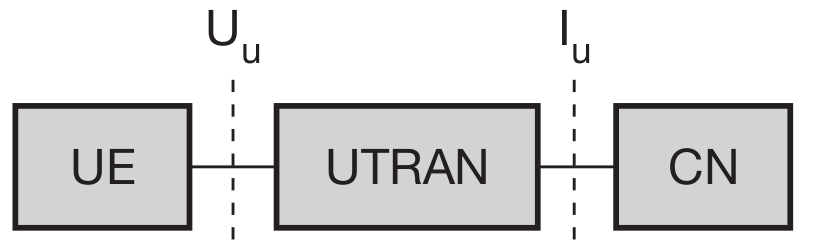
\includegraphics[width=0.6\textwidth]{umts-components}
	\caption{Main components of the UMTS reference architecture}\label{fig:umts-components}
\end{figure}
%-----------------------FIGURE END------------------------



The UMTS network architecture can be divided following elements. Figure \ref{fig:umts-architecture} shows the UMTS architecture.




%%%%%%%%%%%%%%%%%%%%%%%%%%%%%%%%%%%%%%%%%%%%%
%											%
%				Figure						%
%											%
%%%%%%%%%%%%%%%%%%%%%%%%%%%%%%%%%%%%%%%%%%%%%
\begin{figure}[hpt]
	\centering
	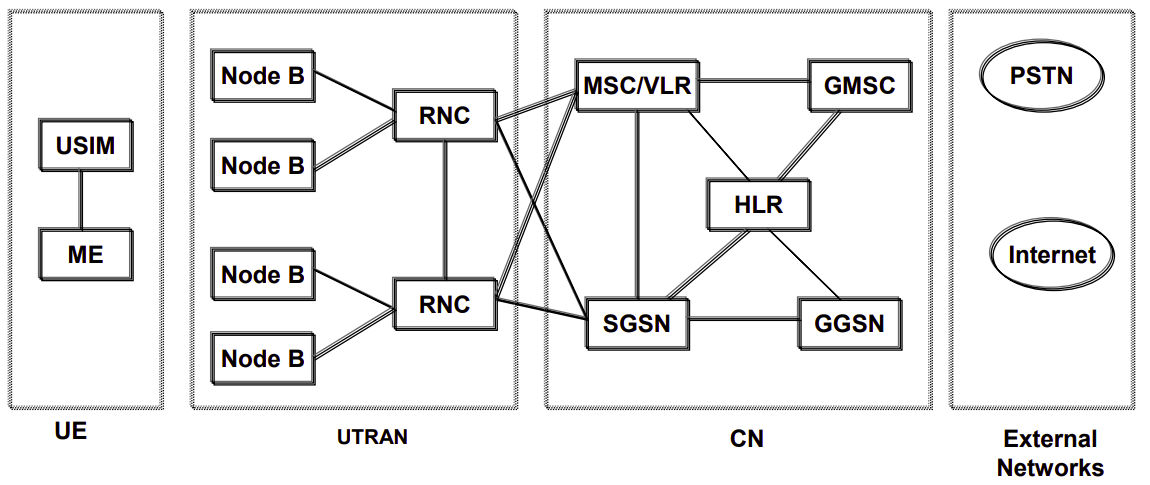
\includegraphics[width=0.9\textwidth]{umts-architecture}
	\caption{UMTS architecture}\label{fig:umts-architecture}
\end{figure}
%-----------------------FIGURE END------------------------
UMTS system composed of three main subsystems:
\begin{itemize}
	\item \textbf{UE (User Equipment)} that interfaces with the user
	\item \textbf{UTRAN (UMTS Terrestrial Radio Access Network)} handles all radio related functionality — WCDMA is radio interface standard here.
	\item \textbf{CN (Core Network)} is responsible for transport functions such as	switching and routing calls and data, tracking users.
\end{itemize}

\subsubsection{UE}
It includes:
\begin{itemize}
	\item ME (Mobile Equipment) and
	\item USIM (UMTS Subscriber Identity Module)
\end{itemize}

\paragraph{ME}
ME is the single or multimode terminal used for radio communication

\paragraph{USIM}
USIM is a smart card that holds the subscriber identity, subscribed services, authentication and encryption keys. 


\subsubsection{UTRAN}
It includes:
\begin{itemize}
	\item Node B
	\item RNC (Radio Network Controller)
\end{itemize}

\paragraph{Node B}
 Node B is equivalent to BTS in GSM/GPRS.
 \begin{itemize}
 	\item It performs the air interface processing (channel coding, rate adaptation, spreading, synchronization, power control).
 	\item It can operate a group of antennas/radios. 
 \end{itemize}

\paragraph{RNC}
RNC is equivalent to GSM BSC.
\begin{itemize}
	\item It is responsible for radio resource management and control of the Node Bs.
	\item Also responsible for handoff decisions, congestion control, power control, encryption, admission control, protocol conversion, etc. 
\end{itemize}


\subsubsection{CN}

\paragraph{HLR}
\begin{itemize}
	\item HLR is a database located in the user’s home system that stores the master copy of the user’s service profile.
	\item The HLR also stores the UE location on the level of MSC and SGSN.
\end{itemize}

\paragraph{3G MSC / VLR}
\begin{itemize}
	\item MSC/VLR are Switch and database that serves the UE in its current location for Circuit Switched (CS) services. 
	\item The MSC function is used to switch the CS	transactions, and VLR function holds a copy of the visiting user’s service
	profile, as well as more precise information on the UE’s location within the serving system
\end{itemize}

\paragraph{3G GMSC}
\begin{itemize}
	\item GMSC is a switch at the point where UMTS is connected to external CS networks. 
	\item All incoming and outgoing CS connections go through GMSC.
\end{itemize}

\paragraph{3G SGSN}
\begin{itemize}
	\item It is similar to that of MSC / VLR but is used for Packet Switched (PS) services.
	\item The part of the network that is accessed via the SGSN is often referred to as	the PS domain. 
	\item Upgrade version of serving GPRS support node.
\end{itemize}

\paragraph{3G GGSN}
\begin{itemize}
	\item GGSN Functionality is close to that of GMSC but is in the relation to PS services.
	\item Upgraded version of gateway GPRS support Node. 
\end{itemize}

\noindent The Core Network (CN) and the Interface $ I_u $ are separated into two logical domains:

\begin{enumerate}
	\item \textbf{Circuit Switched Domain (CSD)}
	\begin{itemize}
		\item Circuit switched service including signaling
		\item Resource reservation at connection setup
		\item 3G versions of GSM components (MSC, GMSC, VLR, HLR)
		\item $ I_u$CS
	\end{itemize}
	
	\item \textbf{Packet Switched Domain (PSD)}
	\begin{itemize}
		\item Handles all packet data services
		\item 3G versions of GPRS components (SGSN, GGSN)
		\item $ I_u $PS
	\end{itemize}

\end{enumerate}
%https://www.electronics-notes.com/articles/connectivity/3g-umts/network-architecture.php
%\begin{itemize}
%	\item \textbf{User Equipment (UE)}: The User Equipment or UE is the name given to what was previous termed the mobile, or cellphone. The new name was chosen because the considerably greater functionality that the UE could have. It could also be anything between a mobile phone used for talking to a data terminal attached to a computer with no voice capability.
%	
%	\item \textbf{Radio Network Subsystem (RNS)}: The RNS also known as the UMTS Radio Access Network, UTRAN, is the equivalent of the previous Base Station Subsystem or BSS in GSM. It provides and manages the air interface fort he overall network.
%	
%	\item \textbf{Core Network}: The core network provides all the central processing and management for the system. It is the equivalent of the GSM Network Switching Subsystem or NSS.
%\end{itemize}
%
%The core network is then the overall entity that interfaces to external networks including the public phone network and other cellular telecommunications networks.

%\subsubsection*{User Equipment, UE}
%The USER Equipment or UE is a major element of the overall 3G UMTS network architecture. It forms the final interface with the user. In view of the far greater number of applications and facilities that it can perform, the decision was made to call it a user equipment rather than a mobile. However it is essentially the handset (in the broadest terminology), although having access to much higher speed data communications, it can be much more versatile, containing many more applications. It consists of a variety of different elements including RF circuitry, processing, antenna, battery, etc.
%
%There are a number of elements within the UE that can be described separately:
%
%\begin{itemize}
%	\item UE RF circuitry:   The RF areas handle all elements of the signal, both for the receiver and for the transmitter. One of the major challenges for the RF power amplifier was to reduce the power consumption. The form of modulation used for W-CDMA requires the use of a linear amplifier. These inherently take more current than non linear amplifiers which can be used for the form of modulation used on GSM. Accordingly to maintain battery life, measures were introduced into many of the designs to ensure the optimum efficiency.
%	
%	\item Baseband processing:   The base-band signal processing consists mainly of digital circuitry. This is considerably more complicated than that used in phones for previous generations. Again this has been optimised to reduce the current consumption as far as possible.
%	
%	\item Battery:   While current consumption has been minimised as far as possible within the circuitry of the phone, there has been an increase in current drain on the battery. With users expecting the same lifetime between charging batteries as experienced on the previous generation phones, this has necessitated the use of new and improved battery technology. Now Lithium Ion (Li-ion) batteries are used. These phones to remain small and relatively light while still retaining or even improving the overall life between charges.
%	
%	\item Universal Subscriber Identity Module, USIM:   The UE also contains a SIM card, although in the case of UMTS it is termed a USIM (Universal Subscriber Identity Module). This is a more advanced version of the SIM card used in GSM and other systems, but embodies the same types of information. It contains the International Mobile Subscriber Identity number (IMSI) as well as the Mobile Station International ISDN Number (MSISDN). Other information that the USIM holds includes the preferred language to enable the correct language information to be displayed, especially when roaming, and a list of preferred and prohibited Public Land Mobile Networks (PLMN).
%	
%	\item The USIM also contains a short message storage area that allows messages to stay with the user even when the phone is changed. Similarly "phone book" numbers and call information of the numbers of incoming and outgoing calls are stored.
%\end{itemize}
%
%The UE can take a variety of forms, although the most common format is still a version of a "mobile phone" although having many data capabilities. Other broadband dongles are also being widely used.
%



\section{LTE}
\subsection{Long Term Evolution}
LTE stands for Long Term Evolution and is a registered trademark owned by ETSI (European Telecommunications Standards Institute) for the wireless data communications technology and a development of the GSM/UMTS standards.

LTE was the 4G successor to the 3G UMTS system which was developed to provide a further evolution of the mobile telecommunications system available.

Providing much higher data speeds and greatly improved performance as well as lower operating costs, the scheme started to be deployed in its basic form around 2008.

Initial deployments gave little improvement over 3G HSPA and were sometimes dubbed 3.5G or 3.99G, but soon the full capability of LTE was realized it provided a full 4G level of performance.

The first deployments were simply known as LTE, but later deployments were designated 4G LTE Advanced and later still 4G LTE Pro.

Not only was the radio access network improved for 4G LTE, but the network architecture was overhauled enabling lower latency and much better interconnectivity between elements of the radio access network, RAN.


LTE is commonly marketed as 4G LTE \& Advance 4G, but it does not meet the technical criteria of a 4G wireless service.	

\subsection{4G}
4G is a collection of fourth generation cellular data technologies. It succeeds 3G and is also called “IMT-Advanced,” or “International Mobile Telecommunications Advanced.”

All 4G standards must conform to a set of specifications created by the International Telecommunications Union. For example, all 4G technologies are required to provide peak data transfer rates of at least 100 Mbps. While actual download and upload speeds may vary based on signal strength and wireless interference, 4G data transfer rates can actually surpass those of cable modem and DSL connections.

Like 3G, there is no single 4G standard. Instead, different cellular providers use different technologies that conform to the 4G requirements.

4G advantages:
\begin{itemize}
	\item high spectral efficiency;
	\item very low latency;
	\item supports variable bandwidths;
	\item simple protocol architecture;
	\item compatibility and interworking with earlier 3GPP releases;
	\item Frequency division duplex (FDD) and time division duplex (TDD) within a single radio access technology;
	\item efficient multicast/broadcast.
\end{itemize}


	\subsection{5G}
	
%The 5G mobile communications system provides a far higher level of performance than the previous generations of mobile communications systems.
%
%The new 5G technology is not just the next version of mobile communications, evolving from 1G to 2G, 3G, 4G, but it provides a new approach giving ubiquitous connectivity.
%
%5G is able to provide much greater flexibility and therefore it is able to support a much wider range of applications, from low data rate Internet of Things requirements through to very fast data rate and very low latency applications.

5G is the 5th generation mobile network. It is a new global wireless standard after 1G, 2G, 3G, and 4G networks. 5G enables a new kind of network that is designed to connect virtually everyone and everything together including machines, objects, and devices.

5G wireless technology is meant to deliver higher multi-Gbps peak data speeds, ultra low latency, more reliability, massive network capacity, increased availability, and a more uniform user experience to more users. Higher performance and improved efficiency empower new user experiences and connects new industries.

5G is based on OFDM (Orthogonal frequency-division multiplexing), a method of modulating a digital signal across several different channels to reduce interference. 5G uses 5G NR air interface alongside OFDM principles. 5G also uses wider bandwidth technologies such as sub-6 GHz and mmWave.

5G will bring wider bandwidths by expanding the usage of spectrum resources, from sub-3 GHz used in 4G to 100 GHz and beyond. 5G can operate in both lower bands (e.\ g.\ , sub-6 GHz) as well as mmWave (e.\ g.\ , 24 GHz and up), which will bring extreme capacity, multi-Gbps throughput, and low latency.

5G is designed to not only deliver faster, better mobile broadband services compared to 4G LTE, but can also expand into new service areas such as mission-critical communications and connecting the massive IoT. This is enabled by many new 5G NR air interface design techniques, such as a new self-contained TDD subframe design


\subsubsection*{Applications of 5G}
5G is used across three main types of connected services, including:
\begin{itemize}
	 \item enhanced mobile broadband, 
	 \item mission-critical communications, and 
	 \item the massive IoT. 
\end{itemize}
A defining capability of 5G is that it is designed for forward compatibility—the ability to flexibly support future services that are unknown today.

5G is designed to deliver peak data rates up to 20 Gbps based on IMT-2020 requirements.


5G technology has developed rapidly. The first real deployments went live in 2019, and further deployments soon followed. Although there were some teething issues, many noticed a significant increase in speed.





 % Chapter-3: Global System For Mobile Communications
% !TeX root = ../wireless_networks.tex
% !TeX spellcheck = en_US

\chapter{Mobile Network Layer}

\section{Mobile IP}
Mobile IP is an IETF standard communications protocol that is designed to allow mobile device users to move from one network to another while maintaining a permanent IP address.

The Mobile IP allows for location-independent routing of IP datagrams on the Internet. Each mobile node is identified by its home address disregarding its current location on the Internet. Mobile IP specifies how a mobile node registers with its home agent and how the home agent routes datagrams to the mobile node through the tunnel.

\subsection{Goals}
\begin{itemize}
\item \textbf{Goal}: Use of mobile computer on the internet.
	\item \textbf{Problem}: As soon as mobile device leaves home network and reconnect at another place, it does not receive a single packet.
	\item \textbf{Reason}: Due to routing mechanisms used on the internet.
\end{itemize}

A host sends an IP packet with the header containing a destination address with other fields. The destination address not only determines the receiver of the packet, but also the physical subnet of the receiver. 

For example, the destination address \texttt{27.36.36.69} shows that the receiver must be connected to the physical subnet with the network prefix \texttt{27.36.36}. 
\begin{itemize}
	\item Routers on the internet now look at the destination addresses of incoming packets and forward them according to internal look-up tables. 
	\item To avoid an explosion of routing tables, only prefixes are stored and further optimizations are applied. 
	\item As long as the receiver can be reached within its physical subnet, it gets the packets; as soon as it moves outside the subnet, a packet will not reach it. 
	\item A host needs a so-called \textbf{topologically correct address}.
\end{itemize}
	
	
\subsection{Assumptions}
This protocol assumes that mobile nodes will generally not change their point of attachment to the Internet more frequently than once per second.

This protocol assumes that IP unicast datagrams are routed based on the destination address in the datagram header (and not, for example,
by source address).
\subsubsection*{Quick `Solutions'}
\begin{itemize}
	\item Assign a new topologically correct IP address to the computer using \gls{dhcp}.
	\item Using dynamic DNS an update of the mapping logical name — IP address is possible.
	\item Using DNS to dynamically adapting the IP address with regard to the current location.
	\item Creation of specific routes to the mobile node.
\end{itemize}
 
\subsubsection*{Problems}
\begin{itemize}
	\item Moving to a new location assigns new IP address which nobody knows and it is almost impossible to find a mobile host on the internet which has just changed its address.
	\item \gls{dns} needs some time before it updates the internal tables necessary to map a logical name to an IP address. This approach does not work if the mobile node moves quite often. The internet and DNS have not been built for frequent updates.
\end{itemize}

There is a severe problem with higher layer protocols like \gls{tcp} which rely on IP addresses. Changing the IP address while still having a \gls{tcp} connection open
means breaking the connection. A \gls{tcp} connection is identified by the tuple (source IP address, source port, destination IP address, destination port), also
known as a \textbf{socket pair} (a socket consists of address and port). Therefore, a \gls{tcp} connection cannot survive any address change. Breaking \gls{tcp} connections is not an
option, using even simple programs like telnet would be impossible. The mobile node would also have to notify all communication partners about the new address.

\subsection{Requirements}
Since the \textit{quick solutions} obviously did not work, a more general architecture had to be designed. Many field trials and proprietary systems finally led to mobile IP as a standard to enable mobility on the internet. Several requirements accompanied the development of the standard:


\subsubsection{Compatibility}
\begin{itemize}
	\item A new standard cannot introduce changes to existing network protocols.
	\item People do not want to change their applications just for mobility.
	\item Mobile has to work with current operating systems.
	\item Mobile IP must not require special media or \gls{mac}/LLC protocols.
	\item Mobile IP has to ensure that users can still access all the other servers and systems	on the internet.
\end{itemize}

\subsubsection{Transparency}

\begin{itemize}
	\item Mobility should remain \textit{invisible} for many higher layer protocols and applications.  
	\item Higher layers should continue to work even if	the mobile computer has changed its point of attachment to the network.
\end{itemize}


\subsubsection{Scalability and Efficiency}
\begin{itemize}
\item Introducing a new mechanism to the internet must not jeopardize its efficiency. 
	\item Enhancing IP for mobility must not generate too many new messages flooding the whole network.
	\item Special care has to be taken considering the lower bandwidth of wireless links.
	\item It is crucial for a mobile IP to be scalable over a large number of participants in the whole internet, worldwide.
\end{itemize}

\subsubsection{Security}
\begin{itemize}
	\item Mobility poses many security problems.
	\item The minimum requirement is that of all the messages related to the management of Mobile IP are authenticated. 
	\item The IP layer must be sure that if it forwards a packet to a mobile host that this host receives the packet.
	\item The IP layer can only guarantee that the IP address of the receiver is correct.
	\item There are no ways of preventing fake IP addresses or other attacks.
\end{itemize}


The goal of a mobile IP can be summarized as: \emph{supporting end-system mobility while maintaining scalability, efficiency, and compatibility in all respects with existing applications and Internet protocols}.


\subsection{Entities and Terminology}
Mobile IP introduces the following entities and terms. Figure \ref{fig:mobile_ip_example}
illustrates an example scenario.

%%%%%%%%%%%%%%%%%%%%%%%%%%%%%
%							%
%		FIGURE				%
%							%
%%%%%%%%%%%%%%%%%%%%%%%%%%%%%

\begin{figure}[ht!]
	\centering
	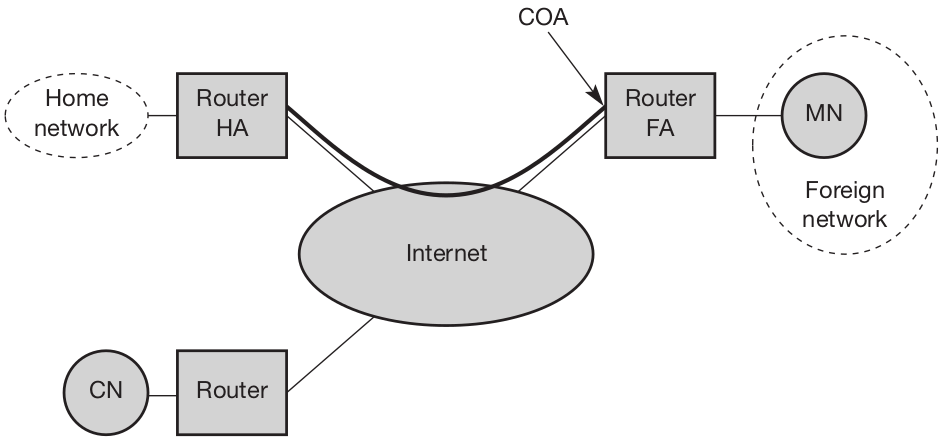
\includegraphics[width=0.7\textwidth]{mobile-ip-example-network}
	\caption{Mobile IP example network}\label{fig:mobile_ip_example}
\end{figure}


\subsection*{Entities}

\subsubsection[Mobile Node]{Mobile Node (MN)}
\begin{itemize}
	\item Is an end-system or router that can change its point of attachment to the internet using mobile IP. 
	\item The MN keeps its IP address and can continuously communicate with any other system on the internet as long as link-layer connectivity is given.
	\item MNs are not necessarily small devices such as laptops with antennas or mobile phones; a router onboard an aircraft can be a powerful mobile node.
\end{itemize}

\subsubsection[Home Agent]{Home Agent (HA)}
\begin{itemize}
	\item The \gls{ha} provides several services for the MN and is located in the home network.
	\item The tunnel for packets toward the MN starts at the \gls{ha}.
	\item The \gls{ha} maintains a location registry, i.\ e.\, it is informed of the MN's location by the current \gls{coa}. 
	\item Three alternatives for the implementation of an \gls{ha} exist:
	\begin{itemize}
			\item On a router that is responsible for the home network.
			\item On an arbitrary node in the subnet.
			\item On the \textit{router} but this time only acting as a manager for MNs belonging to a virtual home network. 
	\end{itemize}
\end{itemize}


\subsubsection[Foreign Agent]{Foreign Agent (FA)}
\begin{itemize}
	\item The \gls{fa} can provide several services to the MN during its visit to the foreign network. 
	\item The \gls{fa} can have the \gls{coa}, acting as tunnel endpoint and forwarding packets to the MN. 
	\item The \gls{fa} can be the default router for the MN. 
	\item \gls{fa}s can also provide security services because they belong to the foreign network as opposed to the MN which is only visiting.
	\item For mobile IP functioning, \gls{fa}s are not necessarily needed. 
	\item Typically, an \gls{fa} is implemented on a router for the subnet the MN attaches to.
\end{itemize}

\subsection*{Terminology}

\subsubsection[Correspondent Node]{Correspondent Node (CN)}
\begin{itemize}
	\item A peer with which a mobile node is communicating.  
	\item A \gls{cn} may be either mobile or stationary.
\end{itemize}

\subsubsection{Home Network}
\begin{itemize}
	\item The home network is the subnet the MN belongs to with respect to its IP address. 
	\item No mobile IP support is needed within the home network.
\end{itemize}

\subsubsection{Foreign Network}
Any network other than the MN's Home Network.

\subsubsection{Home Address}
\begin{itemize}
	\item An IP address that is assigned for an extended period of time to an MN.
	\item It remains unchanged regardless of where the node is attached to the Internet.
\end{itemize}

\subsubsection[Care-of-address]{Care-of-address (COA)}
\begin{itemize}
	\item The COA defines the current location of the MN from an IP point of view. 
	\item All IP packets sent to the MN are delivered to the
	\gls{coa}, not directly to the IP address of the MN. 
	\item Packet delivery toward the MN is done using a tunnel.
	\item There are two different possibilities for the location of the COA:
	
	\begin{itemize}
		\item \textbf{Foreign Agent \gls{coa}}: The \gls{coa} could be located at the \gls{fa}, i.\ e.\, the \gls{coa} is an IP address of the \gls{fa}. The \gls{fa} is the tunnel end-point and forwards packets to the MN.
		\item \textbf{Co-located \gls{coa}}: The \gls{coa} is co-located if the MN temporarily acquired an additional IP address which acts as \gls{coa}. 
	\end{itemize}
\end{itemize}


The example network in Figure \ref{fig:mobile_ip_example} shows the following situation: 
\begin{itemize}
	\item A \gls{cn} is connected via a router to the internet, as are the home network and the foreign network. 
	\item The \gls{ha} is implemented on the router connecting the home network with the internet, an \gls{fa} is implemented on the router to the foreign network.
	\item The MN is currently in the foreign network. 
	\item The tunnel for packets toward the MN starts at the \gls{ha} and ends at the \gls{fa}, for the \gls{fa} has the \gls{coa} in this example.
\end{itemize}


\subsection{IP Packet Delivery}
Figure \ref{fig:packet_delivery_mobile} illustrates packet delivery to and from the MN using the example network of Figure \ref{fig:mobile_ip_example}. 
\begin{steps}
	\item A correspondent node \gls{cn} wants to send an IP packet to the MN. \gls{cn} does not need to know anything about the MN’s current location and sends the packet as usual to the IP address of MN. This means that \gls{cn} sends an IP packet with MN as a destination address and \gls{cn} as a source address. \label{stp:step1}
	\item The \gls{ha} now intercepts the packet. The packet is encapsulated and tunneled to the \gls{coa}. A new header is put in front of the old IP header showing the \gls{coa} as new destination and \gls{ha} as source of the encapsulated packet. \label{stp:step2}
	\item The foreign agent now decapsulates the packet, i.\ e.\ , removes the additional header, and forwards the original packet with \gls{cn} as source and MN as destination to the MN.\label{stp:step3}
	\item The MN sends the packet as usual with its own fixed IP address as source and \gls{cn}'s address as destination.\label{stp:step4}
\end{steps}

The router with the \gls{fa} acts as default router and forwards the packet in the same way as it would do for any other node in the foreign network. As long as \gls{cn} is a fixed node the remainder is in the fixed internet as usual. If \gls{cn} were also a mobile node residing in a foreign network, the same mechanisms as described in \ref{stp:step1} through \ref{stp:step3} would apply now in the other direction.
%%%%%%%%%%%%%%%%%%%%%%%%%%%%%
%							%
%		FIGURE				%
%							%
%%%%%%%%%%%%%%%%%%%%%%%%%%%%%
	
\begin{figure}[hpt]
	\centering
	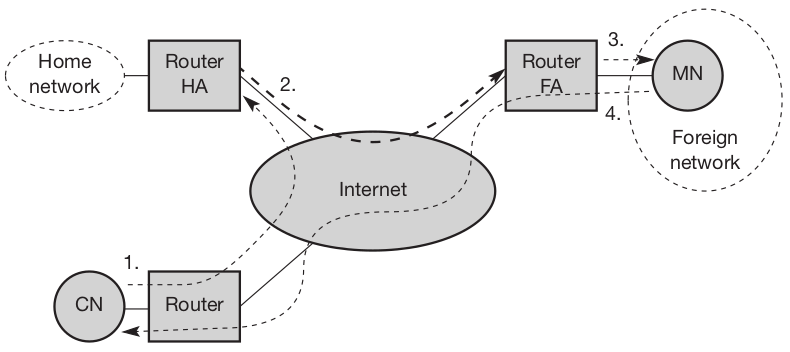
\includegraphics[width=0.8\textwidth]{packet-delivery-mobile}
	\caption{Packet delivery to and from the mobile node}\label{fig:packet_delivery_mobile}
\end{figure}


\subsection*{Working of Mobile IP}
Mobile IP has two addresses for a mobile host: \textit{one home address} and \textit{one care-of address}. 

\begin{itemize}
	\item The home address is permanent; the care-of addresses changes as the mobile host moves from one network to another. 
	\item To make the change of address transparent to the rest of the Internet requires a home agent and a foreign agent. 
	\item The specific function of an agent is performed in the application layer. 
	\item When the mobile host and the foreign agent are the same, the care-of address is called a co-located care-of address. 
	\item To communicate with a remote host, a mobile host goes through three phases:
	\begin{enumerate}
		\item agent discovery, 
		\item registration, and 
		\item data transfer.
	\end{enumerate}
	 
\end{itemize}


\subsection{Agent Discovery}
One initial problem of an MN after moving is how to find a foreign agent. How does the MN discover that it has moved? For this purpose mobile IP describes two methods: 

\begin{itemize}
\item \textit{agent advertisement} and 
\item \textit{agent solicitation},
\end{itemize}
which are in fact router discovery methods plus extensions.

\subsubsection{Agent Advertisement}
For the first method, foreign agents and home agents advertise their presence periodically using special agent \textit{advertisement messages}. These advertisement messages can be seen as a beacon broadcast into the subnet. For these advertisements \gls{icmp} messages are used with some mobility extensions. Routers in the fixed network implementing this standard also advertise their routing service periodically to the attached links.

%%%%%%%%%%%%%%%%%%%%%%%%%%%%%
%							%
%		FIGURE				%
%							%
%%%%%%%%%%%%%%%%%%%%%%%%%%%%%
	
	\begin{figure}[ht!]
	\centering
	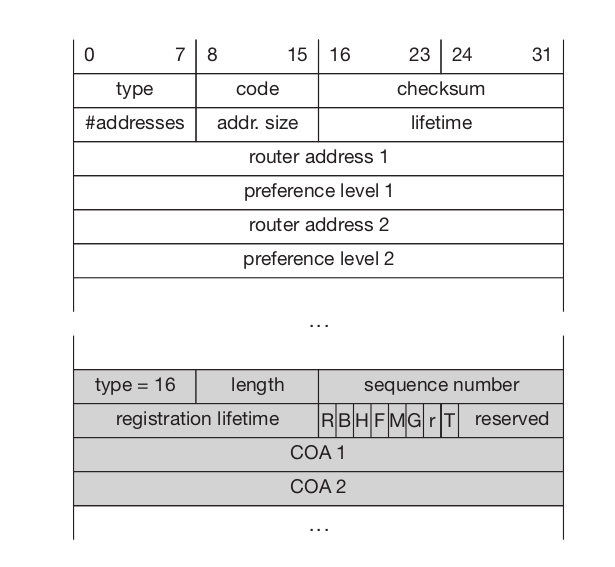
\includegraphics[width=0.8\textwidth]{agent-advertisement-packet}
	\caption[Agent advertisement packet.]{Agent advertisement packet (RFC 1256 + mobility extension)}\label{fig:agent_advertisement}
	\end{figure}
	
	
The agent advertisement packet with the extension for mobility is shown in Figure \ref{fig:agent_advertisement}. 
\begin{itemize}
	\item The upper part represents the \textit{\gls{icmp} packet}.
	\item The lower part is the \textit{extension needed for mobility}.
\end{itemize}
 The fields necessary on lower layers for the agent advertisement are not shown in this figure. Clearly, mobile nodes must be reached with the appropriate link layer address. The TTL field of the IP packet is set to 1 for all advertisements to avoid forwarding them.

The IP destination address according to standard router advertisements can be either set to \verb|224.0.0.1|, which is the multicast address for all systems on a link, or to the broadcast address \verb|255.255.255.255|.

The fields in the \gls{icmp} part are defined as follows. 

\begin{multicols}{2}
\begin{enumerate}
	\item The \textbf{type} is set to 9.
	
	\item the \textbf{code} can be 0, if the agent also routes traffic from non-mobile nodes, or 16, if it does not route anything other than mobile traffic.
	
	\item \textbf{Lifetime} denotes the length of time this advertisement is valid.
	
	\item Foreign agents are at least required to forward packets from the mobile node. The number of addresses advertised with this packet is in \textbf{\#addresses}.
	
	\item \textbf{Preference} levels for each address help a node to choose the router that is the most eager one to get a new node.
\end{enumerate}
\end{multicols}



The difference compared with standard ICMP advertisements is what happens after the router addresses. This extension for mobility has the following
fields defined:

\begin{multicols}{2}
	\begin{enumerate}
		\item \textbf{type} is set to 16.
		
		\item \textbf{length} depends on the number of COAs provided with the message and equals $ 6 + 4*(number of addresses) $.
		
		\item An agent shows the total number of advertisements sent since initialization in the \textbf{sequence number}.
		
		\item By the \textbf{registration lifetime} the agent can specify the maximum lifetime in seconds a node can request during registration.
	\end{enumerate}
\end{multicols}


The following bits specify the characteristics of an agent in detail.
	
	\begin{multicols}{2}
			\begin{enumerate}
			\item The \textbf{R} bit (registration) shows, if a registration with this agent is required even when using a co-located COA at the MN
			
			\item If the agent is currently too busy to accept new registrations it can set the \textbf{B} bit
			
			\item The following two bits denote if the agent offers services as a home agent \textbf{(H)} or foreign agent \textbf{(F)} on the link where the advertisement has been sent.
			
			\item Bits \textbf{M} and \textbf{G} specify the method of encapsulation used for the tunnel.
			
			\item \textbf{M} can specify minimal encapsulation and \textbf{G} generic routing encapsulation.
			
			\item In the first version of mobile IP the \textbf{V} bit specified the use of header compression
			
			\item Now the field \textbf{r} at the same bit position is set to zero and must be ignored.
			
			\item The new field \textbf{T} indicates that reverse tunneling is supported by the FA.
		\end{enumerate}
	\end{multicols}


The following fields contain the \textbf{COAs} advertised:
\begin{itemize}
\item A foreign agent setting the F bit must advertise at least one COA.
\end{itemize}

A mobile node in a subnet can now receive agent advertisements from either its home agent or a foreign agent. This is one way for the MN to discover its location.

\subsubsection{Agent Solicitation}
\begin{itemize}
\item If no agent advertisements are present or the inter-arrival time is too high, and an MN has not received a \gls{coa} by other means, e.\ g.\, \gls{dhcp}, the mobile node must send \textbf{agent solicitations}. 

\item Care must be taken to ensure that these solicitation messages do not flood the network, but basically an MN can search for an \gls{fa} endlessly sending out solicitation messages

\item Typically, a mobile node can send out three solicitations, one per second, as soon as it enters a new network.

\item If a node does not receive an answer to its solicitations it must decrease the rate of solicitations exponentially to avoid flooding the network until it reaches a maximum interval between solicitations.


\item Discovering a new agent can be done anytime, not just if the MN is not connected to one.

\item After these steps of advertisements or solicitations the MN can now receive a \gls{coa}, either one for an \gls{fa} or a co-located \gls{coa}. 

\item The MN knows its location (home network or foreign network) and the capabilities of the agent.

\item The next step for the MN is the registration with the \gls{ha} if the MN is in a foreign network.
\end{itemize}


\subsection{Registration}
Having received a COA, the MN has to register with the HA. The main purpose of the registration is to inform the HA of the current location for correct forwarding of packets. Registration can be done in two different ways depending on the location of the COA.

\subsubsection[COA at FA]{COA at The FA}
If the COA is at the FA, registration is done as illustrated in Figure \ref{fig:mobile_node_registration} (left).

\begin{itemize}
	\item The MN sends its registration request containing the COA (see Figure \ref{fig:registration-request}) to the FA which is forwarding the request to the HA.
	\item The HA now sets up a \textbf{mobility binding} containing the mobile node’s home IP address and the current COA. 
	\item Additionally, the mobility binding contains the lifetime of the registration which is negotiated during the registration process. 
	\item Registration expires automatically after the lifetime and is deleted; so, an MN should re-register before expiration. 
	\item This mechanism is necessary to avoid mobility	bindings which are no longer used. 
	\item After setting up the mobility binding, the HA sends a reply message back to the FA which forwards it to the MN.
\end{itemize}


\subsubsection[Co-located COA]{COA is Co-located}
If the COA is co-located, registration can be simpler, as shown in Figure \ref{fig:mobile_node_registration} (right).
\begin{itemize}
	\item The MN may send the request directly to the HA and vice versa.
	\item This is also the registration procedure for MNs returning to their home network. 
	\item Here, they also register directly with the HA. 
	\item However, if the MN received an agent advertisement from the FA it should register via	this FA if the \textbf{R} bit is set in the advertisement.
\end{itemize}

%%%%%%%%%%%%%%%%%%%%%%%%%%%%%
%							%
%		FIGURE				%
%							%
%%%%%%%%%%%%%%%%%%%%%%%%%%%%%

\begin{figure}[hb!]
	\centering
	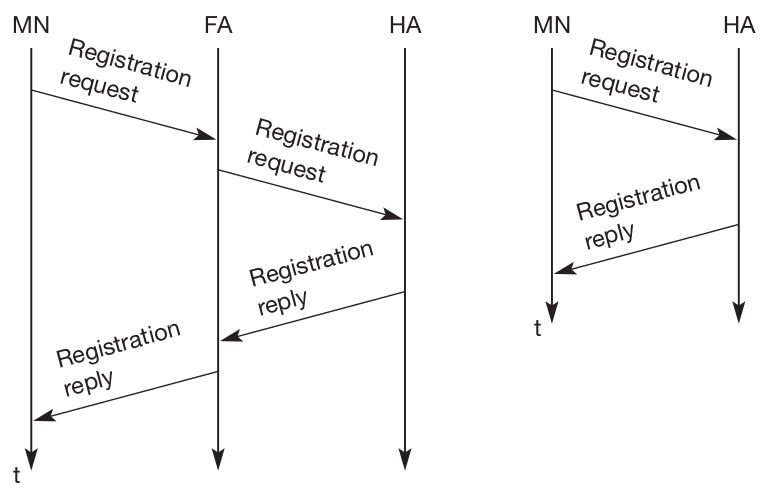
\includegraphics[width=0.8\textwidth]{mobile-node-registration}
	\caption{Registration of a mobile node via the FA or directly with the HA}\label{fig:mobile_node_registration}
\end{figure}



\subsubsection*{Registration Request}
UDP packets are used for \textbf{registration requests}. The IP source address of the packet is set to the interface address of the MN, the IP destination address is that of the FA or HA (depending on the location of the COA). The UDP destination port is set to 434. UDP is used because of low overheads and better performance
compared to \gls{tcp} in wireless environments. The fields relevant for mobile IP registration requests follow as UDP data (see Figure \ref{fig:registration-reply}). The fields are defined as follows.


This allows for simultaneous bindings. The following bits denote the requested behavior for packet forwarding.

%%%%%%%%%%%%%%%%%%%%%%%%%%%%%
%							%
%		FIGURE				%
%							%
%%%%%%%%%%%%%%%%%%%%%%%%%%%%%

\begin{figure}[pht]
	\centering
	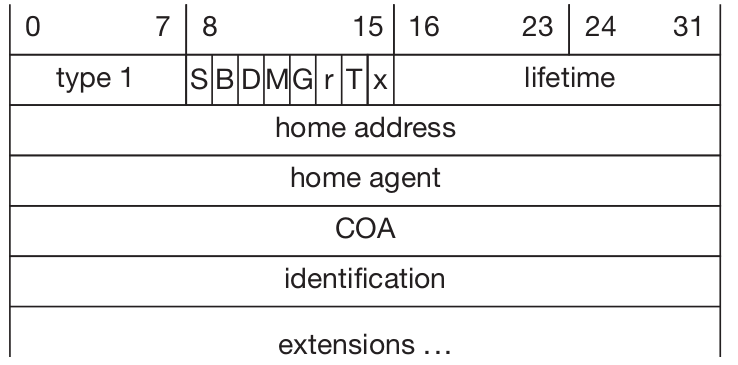
\includegraphics[width=0.8\textwidth]{registration-request}
	\caption{Registration request}\label{fig:registration-request}
\end{figure}

\begin{multicols}{2}
\begin{enumerate}
	\item The first field type is set to 1 for a registration request
	
	\item With the \textbf{S} bit an MN can specify if it wants the HA to retain prior mobility bindings
	
	\item Setting the B bit generally indicates that an MN also wants to receive the broadcast packets which have been received by the HA in the home
	network
	
	\item If an MN uses a co-located COA, it also takes care of the decapsulation at the tunnel endpoint. The \textbf{D} bit indicates this behavior
	
	\item \textbf{M} and \textbf{G} denote the use of minimal encapsulation or generic routing encapsulation, respectively
	
	\item \textbf{T} indicates reverse tunneling
	
	\item \textbf{r} and \textbf{x} are set to zero
	
	\item \textbf{lifetime} denotes the validity of the registration in seconds
	
	\item A value of zero indicates de-registration; all bits set indicates infinity
	
	\item The \textbf{home address} is the fixed IP address of the MN
	
	\item \textbf{home agent} is the IP address of the HA, and COA represents the tunnel endpoint
	
	\item The 64 bit \textbf{identification} is generated by the MN to identify a request and match it with registration replies. This field is used for protection against replay attacks of registrations.
	
	\item The extensions must at least contain parameters for authentication
\end{enumerate}
\end{multicols}


\subsubsection*{Registration Reply}

%%%%%%%%%%%%%%%%%%%%%%%%%%%%%
%							%
%		FIGURE				%
%							%
%%%%%%%%%%%%%%%%%%%%%%%%%%%%%
	
	\begin{figure}[hb!]
	\centering
	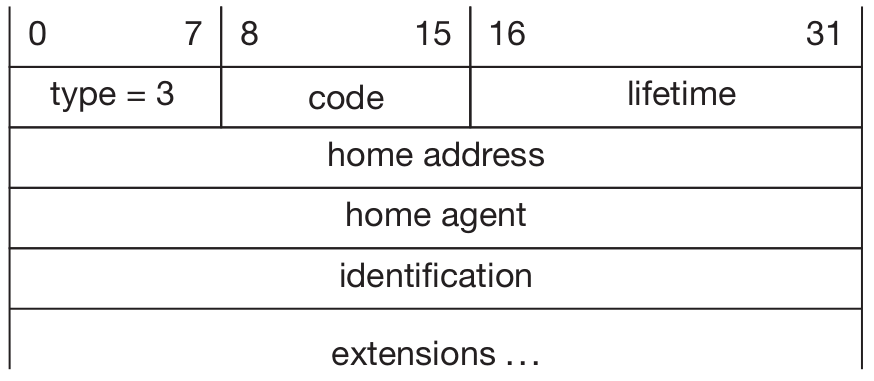
\includegraphics[width=0.8\textwidth]{registration-reply}
	\caption{Registration reply}\label{fig:registration-reply}
	\end{figure}
	
A \textbf{registration reply}, which is conveyed in a UDP packet, contains:
\begin{multicols}{2}
\begin{enumerate}
	\item a \textbf{type} field set to 3 and
	
	\item a \textbf{code} indicating the result of the registration request.
	
	\item \textbf{lifetime} field indicates how many seconds the registration is valid if it was successful.
	
	\item \textbf{home address} and \textbf{home agent} are the addresses of the MN and the HA, respectively.
	
	\item 64-bit \textbf{identification} is used to match registration requests with replies. The value is based on the identification field from the registration and the authentication method.
	
	\item \textbf{extensions} must at least contain parameters for authentication.
	
\end{enumerate}
\end{multicols}

\subsection{Tunneling and Encapsulation}
The following describes the mechanisms used for forwarding packets between the HA and the COA, as shown in Figure \ref{fig:packet_delivery_mobile} \ref{stp:step2} (\textnp{Figure \ref{fig:packet_delivery_mobile} काे \ref{stp:step2} मा Tunneling र Encapsulation को कुरा बताइएको छ।}). 

%%%%%%%%%%%%%%%%%%%%%%%%%%%%%
%							%
%		FIGURE				%
%							%
%%%%%%%%%%%%%%%%%%%%%%%%%%%%%

\begin{figure}[hpt]
	\centering
	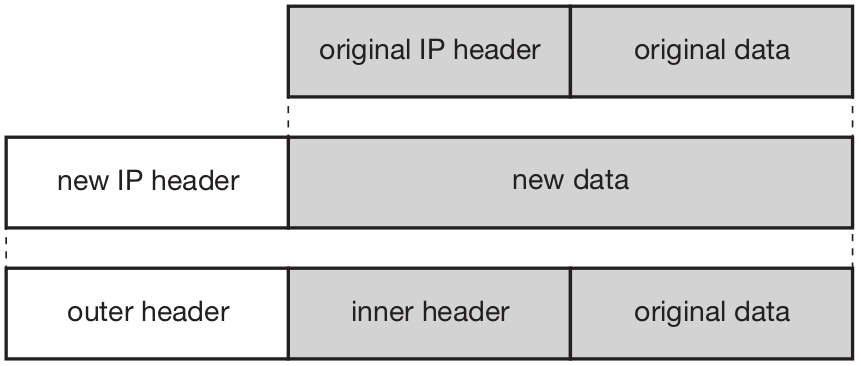
\includegraphics[width=0.7\textwidth]{ip-encapsulation}
	\caption{IP encapsulation}\label{fig:ip_encapsulation}
\end{figure}
%--------------------------------------------------------------------

\subsubsection*{Tunnel}
\begin{multicols}{2}
	\begin{itemize}
		\item A \textbf{tunnel} establishes a virtual pipe for data packets between a tunnel entry and a tunnel endpoint. 
		\item Packets entering a tunnel are forwarded inside the tunnel and leave the tunnel unchanged. 
		\item Tunneling, i.\ e.\ , sending a packet through a tunnel, is achieved by using encapsulation.
	\end{itemize}
\end{multicols}


\subsubsection*{Encapsulation}
\begin{multicols}{2}
\begin{itemize}
	\item \textbf{Encapsulation} is the mechanism of taking a packet consisting of packet header and data and putting it into the data part of a new packet. 
	\item The reverse operation, taking a packet out of the data part of another packet, is called \textbf{decapsulation}. 
	\item Encapsulation and decapsulation are the operations typically performed when a packet is transferred from a higher protocol layer to a lower layer or from a lower to a higher layer respectively. 
	\item Here, these functions are used within the same layer.
\end{itemize}

\end{multicols}


This mechanism is shown in Figure {\ref{fig:ip_encapsulation}} and describes exactly what the HA at the tunnel entry does. 
\begin{multicols}{2}
	\begin{itemize}
		\item The HA takes the original packet with the MN as destination, puts it into the data part of a new packet and sets the new IP header in such a way that the packet is routed to the COA. 
		\item The new header is also called the \textbf{outer header}. 
		\item Additionally, there is an \textbf{inner header} which can be identical to the original header as this is the case for IP-in-IP encapsulation, or the inner header can be computed during encapsulation.
	\end{itemize}
\end{multicols}


\subsubsection{IP-in-IP Encapsulation}
There are different ways of performing the encapsulation needed for the tunnel between HA and COA. Mandatory for mobile IP is \textbf{IP-in-IP encapsulation}. Figure \ref{fig:ip_ip_encapsulation} shows a packet inside the tunnel.

%%%%%%%%%%%%%%%%%%%%%%%%%%%%%
%							%
%		FIGURE				%
%							%
%%%%%%%%%%%%%%%%%%%%%%%%%%%%%

\begin{figure}[hb!]
	\centering
	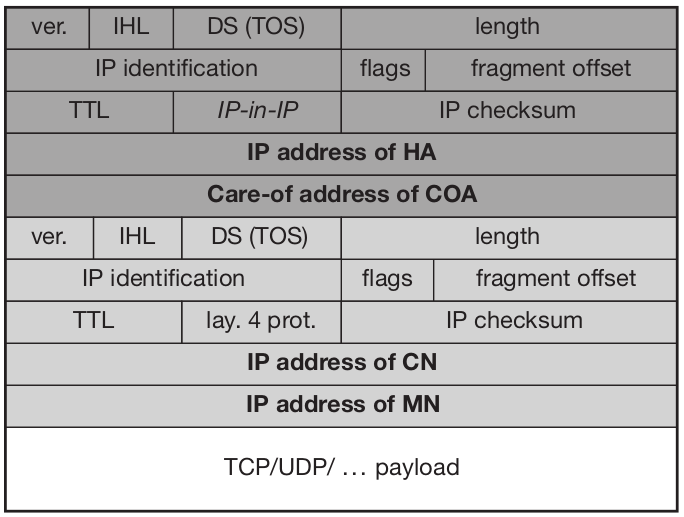
\includegraphics[width=0.8\textwidth]{ip-in-ip-encapsulation}
	\caption{IP-in-IP encapsulation}\label{fig:ip_ip_encapsulation}
\end{figure}


The fields of the outer header are set as follows:
\begin{multicols}{2}
	\begin{itemize}
	\item The version field \textbf{ver} is 4 for IP version 4, the internet header length (IHL) denotes the length of the outer header in 32 bit words.
	
	\item \textbf{DS (TOS)} is just copied from the inner header
	
	\item the \textbf{length} field covers the complete encapsulated packet.
	
	\item TTL have no special meaning for mobile IP.
	
	\item \textbf{TTL} must be high enough so the packet can reach the tunnel endpoint.
	
	\item field, \textbf{IP-in-IP}, is the type of the protocol used in the IP payload. This field is set to 4, the protocol type for IPv4 because again an IPv4 packet follows after this outer header.
	
	\item IP \textbf{checksum} is calculated as usual.
	
	\item the \textbf{IP address of the HA} is the tunnel entry as source address.
	
	\item \textbf{the COA} is the tunnel exit point as destination address
\end{itemize}
\end{multicols}

	
If no options follow the outer header, the inner header starts with the same fields as just explained. This header remains almost unchanged during encapsulation, thus showing the original sender CN and the receiver MN of the packet.

The only change is TTL which is decremented by 1. This means that the whole tunnel is considered a single hop from the original packet’s point of view. This is a very important feature of tunneling as it allows the MN to behave as if it were attached to the home network. No matter how many real hops the packet has to take in the tunnel, it is just one (logical) hop away for the MN. Finally, the payload follows the two headers.



\subsubsection{Minimal encapsulation}


As seen with IP-in-IP encapsulation, several fields are redundant. For example, TOS is just copied, fragmentation is often not needed etc.  \textbf{Minimal encapsulation} (shown in Figure \ref{fig:minimal-encapsulation}) is an optional encapsulation method for mobile IP. 
\begin{multicols}{2}
	\begin{itemize}
		\item The tunnel entry point and endpoint are specified. 
		\item In this case, the field for the type of the following header contains the value 55 for the minimal encapsulation protocol. 
		\item The inner header is different	for minimal encapsulation. 
		\item The type of the following protocol and the address of the MN are needed. 
		\item If the \textbf{S} bit is set, the original sender address of the CN is included as omitting the source is quite often not an option. 
		\item No field for fragmentation offset is left in the inner header and minimal encapsulation does not work with already fragmented packets.
	\end{itemize}
\end{multicols}

%%%%%%%%%%%%%%%%%%%%%%%%%%%%%
%							%
%		FIGURE				%
%							%
%%%%%%%%%%%%%%%%%%%%%%%%%%%%%

\begin{figure}[ht!]
	\centering
	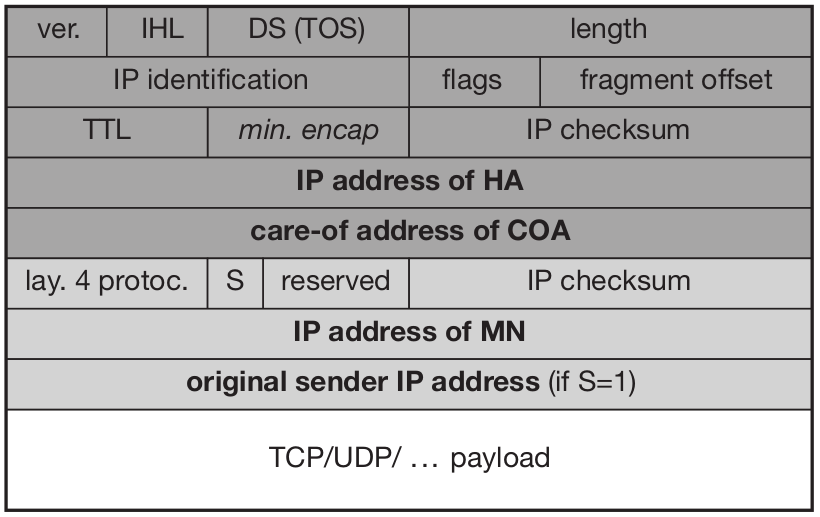
\includegraphics[width=0.8\textwidth]{minimal-encapsulation} 
	\caption{Minimal encapsulation}
	\label{fig:minimal-encapsulation}
\end{figure}

\subsubsection{Generic Routing Encapsulation}
While IP-in-IP encapsulation and minimal encapsulation work only for IP, the encapsulation scheme also supports other network layer protocols in addition to IP. \textbf{Generic routing encapsulation (GRE)} allows the encapsulation of packets of one protocol suite into the payload portion of a packet of another
protocol suite. Figure \ref{fig:generic-routing-encapsulation} shows this procedure. 

%%%%%%%%%%%%%%%%%%%%%%%%%%%%%
%							%
%		FIGURE				%
%							%
%%%%%%%%%%%%%%%%%%%%%%%%%%%%%

\begin{figure}[hb!]
	\centering
	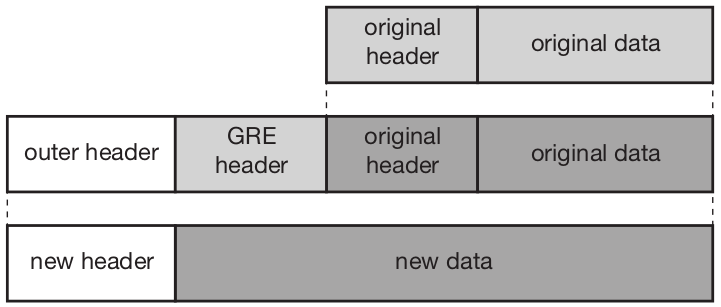
\includegraphics[width=0.8\textwidth]{generic-routing-encapsulation}
	\caption{Generic routing encapsulation}\label{fig:generic-routing-encapsulation}
\end{figure}

\begin{itemize}
	\item The packet of one protocol suite with the original packet header and data is taken and a new GRE header is prepended. 
	\item Together this forms the new data part of the new	packet. 
	\item Finally, the header of the second protocol suite is put in front.
\end{itemize}


\ref{fig:protocol-fields-for-gre} shows on the left side the fields of a packet inside the tunnel
between home agent and COA using GRE as an encapsulation scheme. The outer header is the standard IP header with HA as source
address and COA as destination address. The protocol type used in this outer IP header is 47 for GRE. The other fields of the outer packet, such as TTL and TOS,
may be copied from the original IP header. However, the TTL must be decremented by 1 when the packet is decapsulated to prevent indefinite forwarding.

%%%%%%%%%%%%%%%%%%%%%%%%%%%%%
%							%
%		FIGURE				%
%							%
%%%%%%%%%%%%%%%%%%%%%%%%%%%%%
	
	\begin{figure}[ht!]
	\centering
	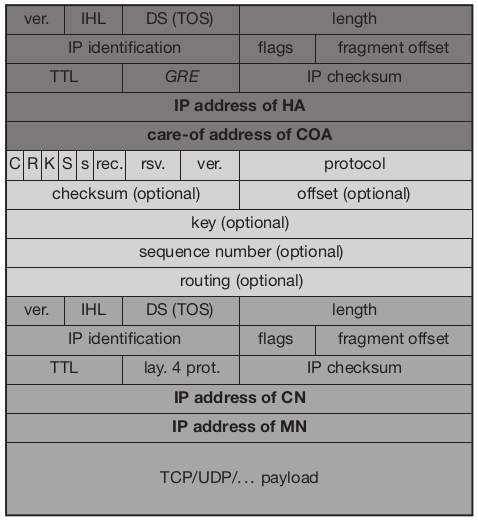
\includegraphics[width=0.8\textwidth]{protocol-fields-for-gre}
	\caption{Protocol fields for GRE}\label{fig:protocol-fields-for-gre}
	\end{figure}
	
The GRE header starts with several flags indicating if certain fields are pre sent or not. A minimal GRE header uses only 4 bytes; nevertheless, GRE is
flexible enough to include several mechanisms in its header. The C bit indicates
if the checksum field is present and contains valid information. 
\begin{multicols}{2}
	\begin{itemize}
		\item If \textbf{C} is set, the	\textbf{checksum} field contains a valid IP checksum of the GRE header and the payload. 
		\item The \textbf{R} bit indicates if the offset and routing fields are present and contain	valid information.
		\item The \textbf{offset} represents the offset in bytes for the first source \textbf{routing} entry. 
		\item The routing field, if present, has a variable length and contains fields for source routing.
		\item \textbf{key} field may be used for authentication. If this field is present, the \textbf{K} bit is set.
		\item The \textbf{sequence} number bit \textbf{S} indicates if the sequence number field is present, if the s bit is set, strict source routing is used. 
		\item The \textbf{recursion control} field (\textbf{rec.}) distinguishes GRE from IP-in-IP and minimal encapsulation. 
		\item The \textbf{reserved} fields must be zero and are ignored on reception. 
		\item The \textbf{version} field contains 0 for the GRE version. 
		\item The 2 byte \textbf{protocol} field represents the protocol of the packet following the GRE header. 
	\end{itemize}
\end{multicols}

	
Figure \ref{fig:protocol-fields-for-gre-rfc-2784} shows the simplified header of GRE, which is a more generalized version of GRE.

This version does not address mutual encapsulation and ignores several protocol-specific nuances on purpose. 

\begin{multicols}{2}
	\begin{itemize}
		\item The field \textbf{C} indicates if a checksum is present. 
		\item The next 5 bits are set to zero, then 7 reserved bits follow. 
		\item The \textbf{version} field contains the value zero. 
		\item The protocol type, defines the protocol of the payload. 
		\item If the flag C is set,	then \textbf{checksum} field and a field called \textbf{reserved1} follows. 
		\item The reserved1 field is constant zero set to zero follow.
	\end{itemize}
\end{multicols}

%%%%%%%%%%%%%%%%%%%%%%%%%%%%%
%							%
%		FIGURE				%
%							%
%%%%%%%%%%%%%%%%%%%%%%%%%%%%%

\begin{figure}[ht!]
	\centering
	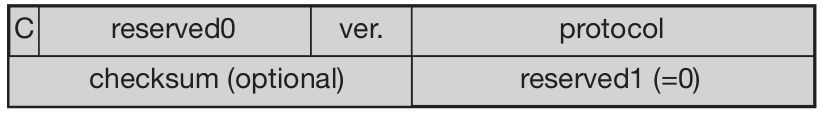
\includegraphics[width=0.8\textwidth]{gre-rfc-2784}
	\caption{Simplified header of GRE}\label{fig:protocol-fields-for-gre-rfc-2784}
\end{figure}

	
\subsection{Optimizations}
Imagine the following scenario. A Nepalese and a Chinese meet at a conference on North Korea. Both want to use their laptops for exchanging data, both run mobile IP for mobility support. Now recall Figure \ref{fig:packet_delivery_mobile} and think of the way the packets between both computers take.

\begin{itemize}
	\item If the Nepalese sends a packet to the Chinese, his computer sends the data to the HA of the Chinese, i.\ e., from North Korea to China. 
	\item The HA in China now encapsulates the packets and tunnels them to the COA of the Chinese laptop on North Korea. 
	\item This means that although the computers might be only meters away, the packets have to travel around the world! This inefficient behavior of a non-optimized mobile IP is called \textbf{triangular routing}. 
	\item The triangle is made of the three segments, CN to HA, HA to COA/MN, and MN back to CN.
\end{itemize}


%With the basic mobile IP protocol all packets to the MN have to go through the HA. This can cause unnecessary overheads for the network between CN and HA, but also between HA and COA, depending on the current location of the MN. As the example shows, latency can increase dramatically. This is particularly unfortunate if the MNs and HAs are separated by, e.g., transatlantic links.


\textbf{Triangle Routing Problem} is considered as one of the problems facing the implementation of Mobile IP. When a CN sends traffics to MN, the following sequence must be done. 
\begin{enumerate}
	\item CN sends packets to the HA.
	\item HA encapsulates these packets and tunnels	them to the FA.
	\item The FA de-tunnels the packets and delivers them to the Mobile Node. 
\end{enumerate}
This behavior is known as triangular routing. As shown in Figure \ref{fig:triangular-routing}, the route taken by these packets is triangle in nature, and the most extreme case of routing can be observed when the Correspondent Node and Mobile Node are in the same subnet.


%%%%%%%%%%%%%%%%%%%%%%%%%%%%%
%							%
%		FIGURE				%
%							%
%%%%%%%%%%%%%%%%%%%%%%%%%%%%%

\begin{figure}[ht!]
	\centering
	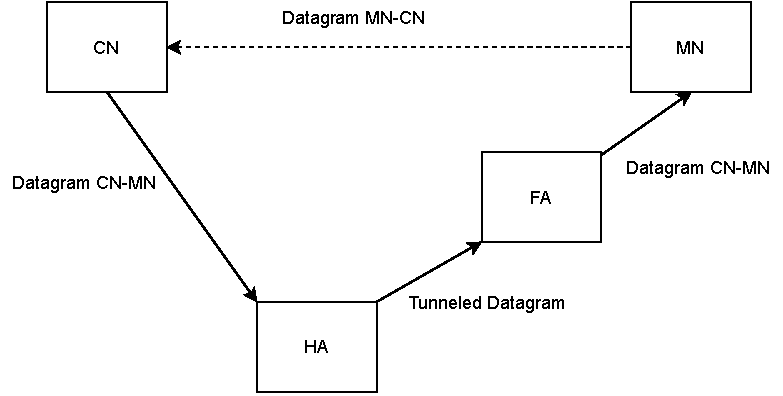
\includegraphics[width=0.8\textwidth]{triangular-routing}
	\caption{Triangular routing}\label{fig:triangular-routing}
\end{figure}

\begin{itemize}
	\item One way to optimize the route is to inform the CN of the current location of the MN. 
	\item The CN can learn the location by caching it in a \textbf{binding cache} which is a part of the local routing table for the CN. 
	\item The appropriate entity to inform the CN of the location is the HA. 
\end{itemize}

The optimized mobile IP protocol needs four additional messages.

\begin{enumerate}
\item \textbf{Binding request}: 
\begin{itemize}
	\item Any node that wants to know the current location of an MN can send a binding request to the HA. 
	\item The HA can check if the MN has allowed dissemination of its current location. 
	\item If the HA is allowed to reveal the location it sends back a binding update.
\end{itemize}

\item \textbf{Binding update}:
\begin{itemize}
	\item This message sent by the HA to CNs reveals the current location of an MN. 
	\item The message contains the fixed IP address of the MN and the COA. 
	\item The binding update can request an acknowledgment.
\end{itemize}


\item \textbf{Binding acknowledgment}: If requested, a node returns this acknowledgment after receiving a binding update message.

\item \textbf{Binding warning}: 
\begin{itemize}
	\item If a node decapsulates a packet for an MN, but it is not the current FA for this MN, this node sends a binding warning. 
	\item The warning contains MN’s home address and a target node address, i.\ e.\, the address of the node that has tried to send the packet to this MN. 
	\item The recipient of the warning then knows that the target node could benefit from obtaining a fresh binding for the MN. 
	\item The recipient can be the HA, so the HA should now send a binding update to the node that obviously has a wrong COA for the MN.
\end{itemize}

\end{enumerate}

Figure \ref{fig:foreign-agent-optimized-mobile-ip} explains these additional four messages together with the case of an MN changing its FA. 

\begin{itemize}
	\item The CN can request the current location from the HA. 
	\item If allowed by the MN, the HA returns the COA of the MN via an update message. 
	\item The CN acknowledges this update message and stores the mobility binding. 
	\item Now the CN can send its data directly to the current foreign agent $FA_{old}$. 
	\item $ FA_{old} $ forwards the packets to the MN. 
	\item This scenario shows a COA located at an FA. 
	\item Encapsulation of data for tunneling to the COA is now done by the CN, not the HA.
\end{itemize}


The MN might now change its location and register with a new foreign agent, $ FA_{new} $. This registration is also forwarded to the HA to update its location database. Furthermore, $ FA_{new} $ informs $ FA_{old} $ about the new registration of MN. MN’s registration message contains the address of $ FA_{old} $ for this purpose. Passing
this information is achieved via an update message, which is acknowledged by $ FA_{old} $. 

Without the information provided by the new FA, the old FA would not get to know anything about the new location of MN. In this case, CN does not know anything about the new location, so it still tunnels its packets for MN to the old FA, $ FA_{old} $. This FA now notices packets with destination MN, but also knows that it is not the current FA of MN. $ FA_{old} $ might now forward these packets to the new COA of MN which is $ FA_{new} $ in this example. This forwarding of packets is another optimization of the basic Mobile IP providing \textbf{smooth handovers}. 

Without this optimization, all packets in transit would be lost while the MN moves from one FA to another. % With \gls{tcp} as the higher layer protocol this would result in severe performance degradation.

%%%%%%%%%%%%%%%%%%%%%%%%%%%%%
%							%
%		FIGURE				%
%							%
%%%%%%%%%%%%%%%%%%%%%%%%%%%%%
	\begin{figure}[ht!]
	\centering
	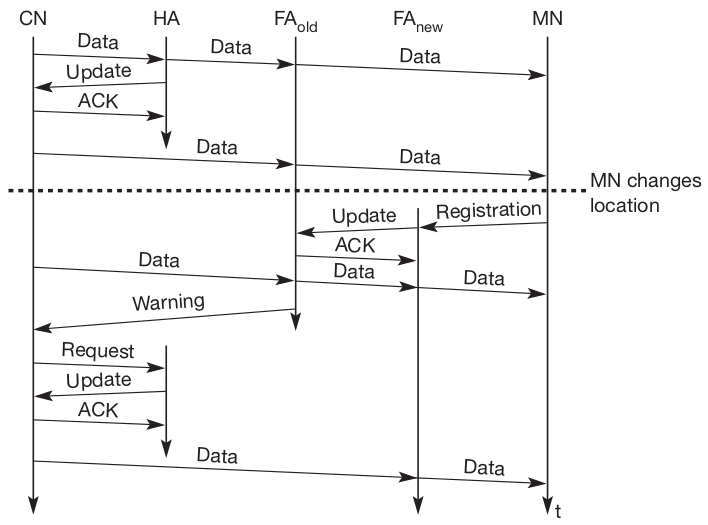
\includegraphics[width=0.8\textwidth]{foreign-agent-optimized-mobile-ip}
	\caption{Change of the foreign agent with an optimized mobile IP}\label{fig:foreign-agent-optimized-mobile-ip}
	\end{figure}

To tell CN that it has a stale binding cache:
\begin{multicols}{2}
	\begin{enumerate}
		\item $ FA_{old} $ sends, a binding warning message to CN. 
		\item CN then requests a binding update. (The warning could also be directly sent to the HA triggering an update). 
		\item The HA sends an update to inform the CN about the new location, which is acknowledged. 
		\item Now CN can send its packets directly to $ FA_{new} $, again avoiding triangular routing. 
	\end{enumerate}
\end{multicols}
	


\subsubsection*{Problems with this optimization}
\begin{multicols}{2}
\begin{itemize}
	\item Security problems such as \textit{tunnel hijacking}.
	\item All users do not want to reveal their current location to others.
\end{itemize}
\end{multicols}



\subsection[DHCP]{Dynamic Host Configuration Protocol (DHCP)}
\begin{itemize}
	\item \gls{dhcp} is an automatic configuration protocol used on IP networks. 
	\item DHCP allows a computer to join an IP-based network without having a pre-configured IP address. 
	\item DHCP is a protocol that assigns unique IP addresses to devices, then releases and renews these addresses as devices leave and re-join the network.
	\item If a new computer is connected to a network, DHCP can provide it with all the necessary information for full system integration into the network, e.\ g.\ , addresses of a DNS server and the default router, the subnet mask, the domain name, and an IP address. 
	\item Providing an IP address, makes DHCP very attractive for mobile IP as a source of care-of-addresses.
\end{itemize}

DHCP is based on a client/server model as shown in Figure \ref{fig:basic-dhcp-config}. DHCP clients send a request to a server (DHCPDISCOVER in the example) to which
the server responds. A client sends requests using MAC broadcasts to reach all devices in the LAN. A DHCP relay might be needed to forward requests across inter-working units to a DHCP server.

%%%%%%%%%%%%%%%%%%%%%%%%%%%%%
%							%
%		FIGURE				%
%							%
%%%%%%%%%%%%%%%%%%%%%%%%%%%%%
	
	\begin{figure}[hb!]
	\centering
	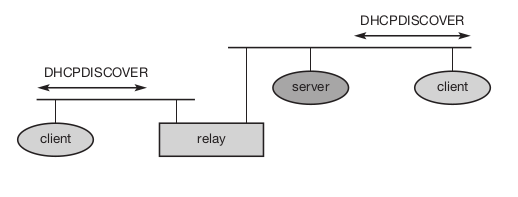
\includegraphics[width=0.8\textwidth]{basic-dhcp-config}
	\caption{Basic DHCP configuration}\label{fig:basic-dhcp-config}
	\end{figure}


A typical initialization of a DHCP client is shown in Figure \ref{fig:dhcp-client-init}. The figure shows one client and two servers. 
\begin{itemize}
	\item The client broadcasts a DHCPDISCOVER into the subnet. There might be a relay to forward this broadcast. 
	\item In the case shown, two servers receive this broadcast and determine the configuration they can offer to the client. 
	\item One example for this could be the checking of available IP addresses and choosing one for the client. 
	\item Servers reply to the client’s request with DHCPOFFER and offer a list of configuration parameters. 
	\item The client can now choose one of the configurations offered.
	\item The client in turn replies to the servers, accepting one of the configurations and rejecting the others using DHCPREQUEST.
	\item If a server receives a DHCPREQUEST with a rejection, it can free the reserved configuration for other possible clients. 
	\item The server with the configuration accepted by the client now confirms the configuration with DHCPACK. This completes the initialization phase.
	
\end{itemize}

If a client leaves a subnet, it should release the configuration received by the server using DHCPRELEASE. Now the server can free the context stored for the client and offer the configuration again. The configuration a client gets from a server is only leased for a certain amount of time, it has to be reconfirmed from time to time. Otherwise the server will free the configuration. This timeout of configuration helps in the case of crashed nodes or nodes moved away without releasing the context.

%%%%%%%%%%%%%%%%%%%%%%%%%%%%%
%							%
%		FIGURE				%
%							%
%%%%%%%%%%%%%%%%%%%%%%%%%%%%%

\begin{figure}[ht!]
	\centering
	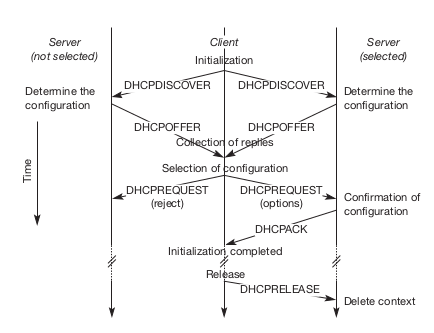
\includegraphics[width=0.8\textwidth]{dhcp-client-init}
	\caption{Client initialization via DHCP}\label{fig:dhcp-client-init}
\end{figure}

%DHCP is a good candidate for supporting the acquisition of care-of-addresses for mobile nodes. The same holds for all other parameters needed, such as addresses of the default router, DNS servers, the timeserver etc. A DHCP server should be located in the subnet of the access point of the mobile node, or at least a DHCP relay should provide forwarding of the messages. RFC 3118 specifies authentication for DHCP messages which is needed to protect mobile nodes from malicious DHCP servers. Without authentication, the mobile node cannot trust a DHCP server, and the DHCP server cannot trust the mobile node.

\subsubsection*{Advantages of DHCP}
\gls{dhcp} provides the following benefits.

\paragraph*{Reliable IP Address Configuration} 
\gls{dhcp} minimizes configuration errors caused by manual IP address configuration, such as typographical errors, or address conflicts caused by the assignment of an IP address to more than one computer at the same time.

\paragraph*{Reduced Network Administration} 
\gls{dhcp} includes the following features to reduce network administration:
\begin{itemize}
	\item Centralized and automated TCP/IP configuration.
	
	\item The ability to define TCP/IP configurations from a central location.
	
	\item The ability to assign a full range of additional TCP/IP configuration values by means of \gls{dhcp} options.
		
	\item The efficient handling of IP address changes for clients that must be updated frequently, such as those for portable devices that move to different locations on a wireless network.
		
	\item The forwarding of initial \gls{dhcp} messages by using a \gls{dhcp} relay agent, which eliminates the need for a \gls{dhcp} server on every subnet.
					
\end{itemize}

 % Chapter-4: Mobile Network Layer
\chapter{Mobile Transport Layer}

Supporting mobility only on lower layers up to the network layer is not enough to provide mobility support for applications. Most applications rely on a transport layer, such as \gls{tcp} or \gls{udp} in the case of the Internet. 

Two functions of the transport layer in the internet are: 
\begin{itemize}
	\item checksumming over user data and 
	\item multiplexing/demultiplexing of data from/to applications.
\end{itemize}

%While the network layer only addresses a host, ports in \gls{udp} or \gls{tcp} allow dedicated applications to be addressed. The connection-less UDP does not offer much more than this addressing, so, the following concentrates on TCP. While UDP is connection-less and
%does not give certain guarantees about reliable data delivery, TCP is much more
%complex and, needs special mechanisms to be useful in mobile environments.
%Mobility support in IP (such as mobile IP) is already enough for UDP to work.
%
%The main difference between UDP and TCP is that TCP offers connections
%between two applications. Within a connection TCP can give certain guarantees, such as in-order delivery or reliable data transmission using retransmission
%techniques. TCP has built-in mechanisms to behave in a ‘network friendly’
%manner. If, for example, TCP encounters packet loss, it assumes network internal congestion and slows down the transmission rate. This is one of the main
%reasons to stay with protocols like TCP. One key requirement for new develop-
%ments in the internet is ‘TCP friendliness'. UDP requires that applications
%handle reliability, in order delivery etc. UDP does not behave in a network
%friendly manner, i.e., does not pull back in case of congestion and continues to
%send packets into an already congested network.


\section{Traditional TCP}
Several mechanisms of the \gls{tcp} that influence the efficiency of \gls{tcp} in a mobile environment are:

\subsection{Congestion Control}

\begin{itemize}
	\item TCP has been designed for fixed networks with fixed end-systems.
	\item Data transmission takes place using network adapters, fiber optics, copper wires, special hardware for routers etc.
	\item Most of the hardware/software is not responsible for lost packets or bits flipping.
	\item The probable reason for a packet loss in a fixed network is a \textit{state of congestion at a node}.
	\item Router drops packets when the packet buffers of a router are filled and router cannot forward the packets fast enough because sum of input rates of packets destined is higher than the capacity of the output.
	\item A dropped packet is lost for the transmission, and the receiver notices a gap in the packet stream.
	\item Receiver does not tell sender if packet is missing, bit continues to acknowledge packets in sequence up to the missing one.
	\item When sender notices missing acknowledgment, it assumes a packet loss due to congestion and re-transmits the missing packet at full speed. This increases congestion.
	\item To mitigate congestion, \gls{tcp} slows down the transmission rate dramatically. 
\end{itemize}

\subsection{Slow Start}
The behavior \gls{tcp} shows after the detection of congestion is called \textit{slow start}.

\begin{itemize}
	\item The sender always calculates a congestion window for a receiver. 
	\item The start size of the congestion window is one segment (\gls{tcp} packet). 
	\item The sender sends one packet and waits for acknowledgment. 
	\item If this acknowledgment arrives, the sender increases the congestion window by one, now sending two packets (congestion window = 2). 
	\item This scheme doubles the congestion window every time the acknowledgments come back, which
	takes \gls{rtt}. 
	\item This is called the exponential growth of the congestion window in the slow start mechanism.
\end{itemize}


The exponential growth stops at the congestion \textit{threshold}. As soon as the congestion window reaches the congestion threshold, further increase of the transmission rate is only linear by adding 1 to the congestion window each time the acknowledgments come back.

Linear increase continues until a time-out at the sender occurs due to a missing acknowledgment, or until the sender detects a gap in transmitted data because of continuous acknowledgments for the same packet. In either case the sender sets the congestion threshold to half of the current congestion window.

%The congestion window itself is set to one segment and the sender starts sending
%a single segment. The exponential growth (as described above) starts once more
%up to the new congestion threshold, then the window grows in linear fashion.


\subsection{Fast Re-transmit/Fast Recovery}
Two things lead to a reduction of the congestion threshold:

\begin{itemize}
	\item One is a sender receiving continuous acknowledgments for the same packet. 
	\begin{itemize}
		\item This informs the sender of two things. One is that the receiver got all packets up to the acknowledged packet in sequence. In TCP, a receiver sends acknowledgments only if it receives any packets from the sender. Receiving acknowledgments from a
		receiver also shows that the receiver continuously receives something from the sender. The gap in the packet stream is not due to severe congestion, but a
		simple packet loss due to a transmission error. The sender can now re-transmit the missing packet(s) before the timer expires. This behavior is called \textit{fast re-transmit}.
		
		\item The receipt of acknowledgments shows that there is no congestion to justify a slow start. The sender can continue with the current congestion window. The sender performs a fast recovery from the packet loss.
	\end{itemize}
	

	\item The other reason for activating slow start is a time-out due to a missing acknowledgment.
\end{itemize} 



\subsection{Implications on Mobility}

\begin{itemize}
	\item \textit{Slow start} decreases the efficiency of \gls{tcp} if used together with mobile receivers
	or senders. The reason being the use slow start under the wrong assumptions.
%	\item From a missing acknowledgment, \gls{tcp} concludes a congestion situation.
	\item Error rates on wireless links are orders of magnitude higher compared to fixed fiber or copper links.
	\item Mobility can cause packet loss. There are many situations where a soft
	handover from one access point to another is not possible for a mobile end system. 
	\item Standard TCP reacts with slow start if acknowledgments are missing, which does not help in the case of transmission errors over wireless links and which does not really help during handover. This behavior results in a severe performance degradation of an unchanged \gls{tcp} if used together with wireless links or mobile nodes.
\end{itemize}

\section{Classical TCP Improvements}
Together with the introduction of \gls{wlan}s in the mid-nineties several research projects were started with the goal to increase \gls{tcp}’s performance in wireless and mobile environments.

\subsection{Indirect TCP (I-TCP)}
Two competing insights led to the development of {I-TCP}:
\begin{itemize}
	\item \gls{tcp} performs poorly together with wireless links.
	\item \gls{tcp} within the fixed network cannot be changed.
\end{itemize}

I-TCP segments a \gls{tcp} connection into:
\begin{multicols}{2}
	\begin{enumerate}[label=\alph*)]
		\item a fixed part and
		\item a wireless part.
	\end{enumerate}
\end{multicols}


Figure \ref{fig:indirect_tcp} shows an example with a mobile host connected via a wireless link and an access point to the ‘wired’ internet where the correspondent host resides. The correspondent node could also use wireless access. 
\begin{itemize}
	\item Standard TCP is used between the fixed computer and the access point. No computer in the internet recognizes any changes to \gls{tcp}. 
	\item Instead of the mobile host, the access point now terminates the standard \gls{tcp} connection, acting as a proxy. 
	\item This means that the access point is now seen as the mobile host for the fixed host and as the fixed host for the mobile host. 
	\item Between the access point and the mobile host, a special \gls{tcp}, adapted to wireless links, is used. 
	\item A good place for segmenting the connection between mobile host and correspondent host is at the foreign agent of mobile IP. 
	\item The foreign agent controls the mobility of the mobile host anyway and can also hand over the connection to the next foreign agent when the mobile host moves on. 
\end{itemize}



%%%%%%%%%%%%%%%%%%%%%%%%%%%%%%%%%%%%%
%									%
%			FIGURE					%
%									%
%%%%%%%%%%%%%%%%%%%%%%%%%%%%%%%%%%%%%

\begin{figure}[ht!]
	\centering
	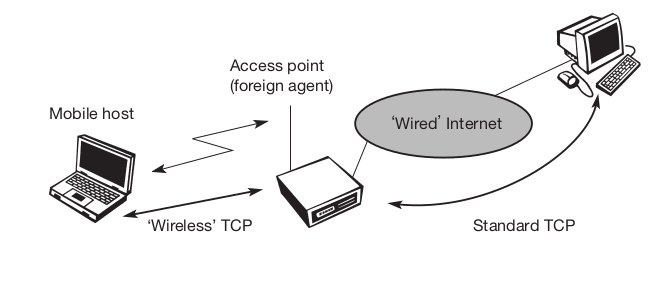
\includegraphics[width=0.8\textwidth]{indirect-tcp}
	\caption{Indirect TCP segments a TCP connection into two parts}\label{fig:indirect_tcp}
\end{figure}


The correspondent host in the fixed network does not notice the wireless link or the segmentation of the connection. The foreign agent acts as a proxy and relays all data in both directions. If the correspondent host sends a packet, the foreign agent acknowledges this packet and tries to forward the packet to the mobile host. If the mobile host receives the packet, it acknowledges the packet. However, this acknowledgment is only used by the foreign agent. If a packet is lost on the wireless link due to a transmission error, the correspondent host would not notice this. In this case, the foreign agent tries to re-transmit this packet locally to maintain reliable data transport.

Similarly, if the mobile host sends a packet, the foreign agent acknowledges this packet and tries to forward it to the correspondent host. If the packet is lost on the wireless link, the mobile hosts notice this much faster due to the lower round trip time and can directly re-transmit the packet. Packet loss in the wired network is now handled by the foreign agent.


\begin{itemize}
	\item I-TCP requires several actions as soon as a handover takes place (see Figure \ref{fig:socket-state-migration}). 
	\item In the example shown, the access point acts as a proxy buffering packets for re-transmission. 
	\item After the handover, the old proxy must forward buffered data to the new proxy because it has already acknowledged the data. 
	\item After registration with the new foreign agent, this new foreign agent can inform the old one about its location to enable packet forwarding. 
	\item Besides buffer content, the sockets of the proxy, too, must migrate to the new foreign agent located in the access point. 
	\item The socket reflects the current state of the \gls{tcp} connection, i.\ e.\, sequence number, addresses, ports etc. No new connection may be
	established for the mobile host, and the correspondent host must not see any changes in connection state.
\end{itemize}


%%%%%%%%%%%%%%%%%%%%%%%%%%%%%%%%%%%%%
%									%
%			FIGURE					%
%									%
%%%%%%%%%%%%%%%%%%%%%%%%%%%%%%%%%%%%%

\begin{figure}[hb!]
	\centering
	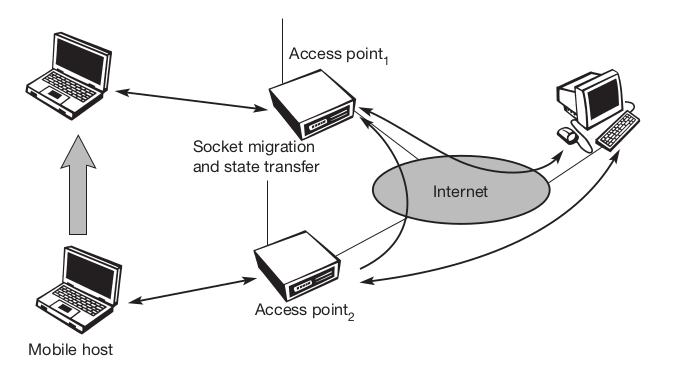
\includegraphics[width=0.8\textwidth]{socket-and-state-migration}
	\caption{Socket and state migration after handover of a mobile host}\label{fig:socket-state-migration}
\end{figure}

\subsubsection[Advantages]{Advantages With I-TCP}
There are several advantages with I-TCP:

\begin{itemize}
	\item I-TCP does not require any changes in the \gls{tcp} protocol.
	\item All current optimizations for \gls{tcp} still work between the foreign agent and the corresponding host.
	
	\item Due to the strict partitioning into two connections, transmission errors on the wireless link, i.\ e.\ , lost packets, cannot propagate into the fixed network.

    \item Introduction to new mechanism into a huge network is always dangerous. I-TCP ensures Different solutions can be tested or used at the same time without jeopardizing the stability of the network.
    
    \item Optimizing new mechanism is simple because they only cover one single hop.
    
	\item An optimized \gls{tcp} could use precise timeouts to guarantee retransmission as fast as possible. 
	
	\item Partitioning into two connections also allows the use of a different transport layer protocol between the foreign agent and the mobile host.
	
\end{itemize}

\subsubsection[Disadvantages]{I-TCP Disadvantages}
Idea of segmentation in I-TCP also comes with some disadvantages:

\paragraph*{Loss of End-to-End Semantics}
 The loss of the end-to-end semantics of \gls{tcp} might cause problems if the foreign agent partitioning the \gls{tcp} connection crashes.
 
 \paragraph*{Handover Latency}
 Increased handover latency may be much more problematic. All packets sent by the correspondent host are buffered by the foreign
 agent besides forwarding them to the mobile host.
 
 \paragraph*{Security Mechanism}
 The foreign agent must be a trusted entity because the \gls{tcp} connections
 end at this point. If users apply end-to-end encryption, e.\ g.\, the foreign agent has to be integrated into all security mechanisms.
 

\subsection{Snooping TCP}
One of the drawbacks of I-TCP is the segmentation of the single \gls{tcp} connection into two \gls{tcp} connections. This loses the original end-to-end \gls{tcp} semantic. The following \gls{tcp} enhancement works completely transparently and leaves the \gls{tcp} end-to-end connection intact.

The main function of the enhancement is to buffer data close to the mobile host to perform fast local re-transmission in case of packet loss.

\begin{itemize}
	\item In this approach, the foreign agent buffers all packets with destination
	mobile host and additionally \textit{snoops} the packet flow in both directions to recognize acknowledgments.
	\item The reason for buffering packets toward the mobile node is to enable the foreign agent to perform a local re-transmission in case of packet loss on the wireless link. 
	\item The foreign agent buffers every packet until it receives an acknowledgment from the mobile host.
	\item If the foreign agent does not receive an acknowledgment from the mobile host within a certain amount of time, either the packet or the acknowledgment has been lost.
	\item Alternatively, the foreign agent could receive a duplicate ACK which also shows the loss of a packet.
	\item Now the foreign agent re-transmits the packet directly from the buffer, performing a much faster re-transmission compared to the correspondent host. 
	\item The time out for acknowledgments can be much shorter, because it reflects only the delay of one hop plus processing time.
	
\end{itemize}


%%%%%%%%%%%%%%%%%%%%%%%%%%%%%
%							%
%		FIGURE				%
%							%
%%%%%%%%%%%%%%%%%%%%%%%%%%%%%

\begin{figure}[ht!]
	\centering
	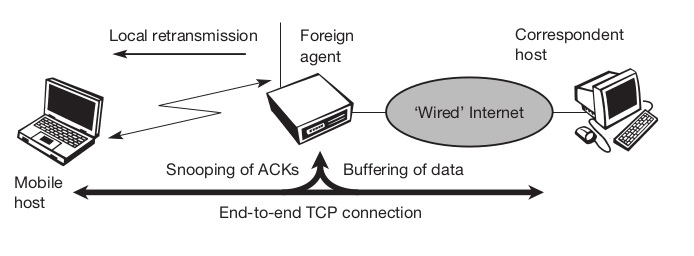
\includegraphics[width=0.9\textwidth]{snooping-tcp}
	\caption{Snooping TCP as a transparent TCP extension}\label{fig:snooping-tcp}
\end{figure}


%To remain transparent, the foreign agent must not acknowledge data to the correspondent host. This would make the correspondent host believe that the mobile host had received the data and would violate the end-to-end semantic in case of a foreign agent failure. However, the foreign agent can filter the duplicate acknowledgments to avoid unnecessary re-transmissions of data from the correspondent host. If the foreign agent now crashes, the time-out of the correspondent host still works and triggers a re-transmission. The foreign agent may discard duplicates of packets already re-transmitted locally and acknowledged by the mobile host. This avoids unnecessary traffic on the wireless link.

Data transfer from the mobile host with destination correspondent host works as follows. 
\begin{itemize}
	\item The foreign agent snoops into the packet stream to detect gaps in the sequence numbers of TCP.
	\item As soon as the foreign agent detects a missing packet, it returns a negative acknowledgment (NACK) to the mobile host. 
	\item The mobile host can now re-transmit the missing packet immediately. 
	\item Reordering of packets is done automatically at the correspondent host by TCP.
	
\end{itemize}


\subsubsection[Advantages]{Advantages of Snooping TCP}
Extending the functions of a foreign agent with a \textit{snooping TCP} has several advantages:

\paragraph*{Preserve End-to-End Semantics}
The end-to-end TCP semantic is preserved. No matter at what time the foreign agent crashes, neither the correspondent host nor the mobile host have an
inconsistent view of the TCP connection as is possible with I-TCP. The approach automatically falls back to standard TCP if the enhancements
stop working.

\paragraph*{Change in Correspondent Host Not Required}
The correspondent host does not need to be changed; most of the enhancements are in the foreign agent. Supporting only the packet stream from the
correspondent host to the mobile host does not even require changes in the mobile host.

\paragraph*{Immediate Handover of State Not Required}
It does not need a handover of state as soon as the mobile host moves to another foreign agent. Assume there might still be data in the buffer not
transferred to the next foreign agent. All that happens is a time-out at the correspondent host and re-transmission of the packets, possibly already to
the new care-of address.

\paragraph*{Automatic Fallback to Standard Solution}
It does not matter if the next foreign agent uses the enhancement or not. If not, the approach automatically falls back to the standard solution. This is one of the problems of I-TCP.

%\begin{itemize}
%	\item The end-to-end TCP semantic is preserved. No matter at what time the foreign agent crashes (if this is the location of the buffering and snooping
%	mechanisms), neither the correspondent host nor the mobile host have an
%	inconsistent view of the TCP connection as is possible with I-TCP. The
%	approach automatically falls back to standard TCP if the enhancements
%	stop working.
%	
%	\item The correspondent host does not need to be changed; most of the enhancements are in the foreign agent. Supporting only the packet stream from the
%	correspondent host to the mobile host does not even require changes in the
%	mobile host.
%	
%	\item It does not need a handover of state as soon as the mobile host moves to
%	another foreign agent. Assume there might still be data in the buffer not
%	transferred to the next foreign agent. All that happens is a time-out at the
%	correspondent host and re-transmission of the packets, possibly already to
%	the new care-of address.
%	
%	\item It does not matter if the next foreign agent uses the enhancement or not. If
%	not, the approach automatically falls back to the standard solution. This is
%	one of the problems of I-TCP, since the old foreign agent may have already
%	signaled the correct receipt of data via acknowledgements to the correspondent host and now has to transfer these packets to the mobile host via the
%	new foreign agent.
%\end{itemize}

\subsubsection[Disadvantages]{Disadvantages of Snooping TCP}
The simplicity of the scheme also results in some disadvantages:

\paragraph*{No Proper Wireless Link Isolation}
Snooping TCP does not isolate the behavior of the wireless link as well as I-TCP. The quality of the isolation, which snooping TCP offers, strongly depends on the quality of the wireless link, time-out values, and further traffic characteristics. It is problematic that the wireless link exhibits very high delays compared to the wired link due to error correction.


\paragraph*{Lack of Transparency}
Using negative acknowledgments between the foreign agent and the mobile host assumes additional mechanisms on the mobile host. This approach is no longer transparent for arbitrary mobile hosts.

\paragraph*{Incompatible With Encryption}
All efforts for snooping and buffering data may be useless if certain encryption schemes are applied end-to-end between the correspondent host and
mobile host. 


%\begin{itemize}
%	\item Snooping TCP does not isolate the behavior of the wireless link as well as I-TCP. Assume, for example, that it takes some time until the foreign agent
%	can successfully retransmit a packet from its buffer due to problems on the
%	wireless link (congestion, interference). Although the time-out in the foreign agent may be much shorter than the one of the correspondent host,
%	after a while the time-out in the correspondent host triggers a retransmission. The problems on the wireless link are now also visible for the correspondent host and not fully isolated. The quality of the isolation, which
%	snooping TCP offers, strongly depends on the quality of the wireless link,
%	time-out values, and further traffic characteristics. It is problematic that the
%	wireless link exhibits very high delays compared to the wired link due to
%	error correction on layer 2 (factor 10 and more higher). This is similar to I-TCP. If this is the case, the timers in the foreign agent and the
%	correspondent host are almost equal and the approach is almost ineffective.
%	
%	
%	\item Using negative acknowledgments between the foreign agent and the
%	mobile host assumes additional mechanisms on the mobile host. This
%	approach is no longer transparent for arbitrary mobile hosts.
%	
%	\item All efforts for snooping and buffering data may be useless if certain encryption schemes are applied end-to-end between the correspondent host and
%	mobile host. Using IP encapsulation security payload the TCP protocol header will be encrypted – snooping on the
%	sequence numbers will no longer work. Retransmitting data from the foreign agent may not work because many security schemes prevent replay
%	attacks – retransmitting data from the foreign agent may be misinterpreted
%	as replay. Encrypting end-to-end is the way many applications work so it is
%	not clear how this scheme could be used in the future. If encryption is used
%	above the transport layer (e.g., SSL/TLS) snooping TCP can be used.
%\end{itemize}


\subsection{Mobile TCP}

Dropping packets due to a handover or higher bit error rates is not the only phenomenon of wireless links and mobility — the occurrence of lengthy and/or frequent disconnections is another problem. Quite often mobile users cannot connect at all. 


%A TCP sender tries to re-transmit data controlled by a re-transmission timer that doubles with each unsuccessful re-transmission attempt, up to a maximum of one minute (the initial value depends on the round trip time). This means that the sender tries to retransmit an unacknowledged packet every minute and will give up after 12 retransmissions. What happens if connectivity is back earlier than this? No data is successfully transmitted for a period of one minute! The retransmission time-out is still valid and the sender has to wait. The sender also goes into slow-start because it assumes congestion.

%What happens in the case of I-TCP if the mobile is disconnected? The proxy has to buffer more and more data, so the longer the period of disconnection, the more buffer is needed. If a handover follows the disconnection, which is typical, even more state has to be transferred to the new proxy. The snooping approach also suffers from being disconnected. The mobile will not be able to send ACKs so, snooping cannot help in this situation.

The \textbf{M-TCP (mobile TCP)}\footnote{Mobile TCP does not have the same status as mobile IP, which is an internet RFC.} approach has the same goals as I-TCP and snooping TCP: 
\begin{itemize}
	\item to prevent the sender window from shrinking if bit errors or disconnection but not congestion cause current problems.
\end{itemize}

M-TCP wants to improve overall throughput:

\begin{itemize}
	\item to lower the delay, 
	\item to maintain end-to-end semantics of TCP, and 
	\item to provide a more efficient handover. 
\end{itemize}


Additionally, M-TCP is especially adapted to the problems arising from lengthy or frequent disconnections.

M-TCP splits the TCP connection into two parts as I-TCP does. 
\begin{itemize}
	\item An unmodified TCP is used on the standard host-supervisory host (SH) connection, 
	\item while an optimized TCP is used on the SH-MH connection.
\end{itemize}


The supervisory host is responsible for exchanging data between both parts similar to the proxy in I-TCP (see Figure \ref{fig:indirect_tcp}). The M-TCP approach assumes a relatively low bit error rate on the wireless link. Therefore, it does not perform caching/re-transmission of data via the SH. If a packet is lost on the wireless link, it has to be re-transmitted by the original sender. This maintains the TCP end-to-end semantics.

\begin{itemize}
	\item The SH monitors all packets sent to the MH and ACKs returned from the MH. 
	\item If the SH does not receive an ACK for some time, it assumes that the MH is disconnected. It then chokes the sender by setting the sender’s window size to 0.
	\item Setting the window size to 0 forces the sender to go into \textit{persistent mode}, i.\ e.\ ,
	the state of the sender will not change no matter how long the receiver is disconnected. This means that the sender will not try to retransmit data. 
	\item As soon as the SH (either the old SH or a new SH) detects connectivity again, it reopens the window of the sender to the old value. 
	\item The sender can continue sending at full speed. 
	\item This mechanism does not require changes to the sender’s TCP.
\end{itemize}
The wireless side uses an adapted TCP that can recover from packet loss much faster. This modified TCP does not use slow start, thus, M-TCP needs a bandwidth manager to implement fair sharing over the wireless link.

\subsubsection[Advantages]{Advantages of M-TCP}
The advantages of M-TCP are the following:

\paragraph*{Maintains TCP End-to-End Semantics}
It maintains the TCP end-to-end semantics. The SH does not send any ACK
itself but forwards the ACKs from the MH.

\paragraph*{Avoids Useless Re-transmissions}
If the MH is disconnected, it avoids useless re-transmissions, slow starts or
breaking connections by simply shrinking the sender’s window to 0.

\paragraph*{Does Not Buffer Data}
Since it does not buffer data in the SH as I-TCP does, it is not necessary to
forward buffers to a new SH. Lost packets will be automatically retransmitted to the new SH.

%\begin{itemize}
%	\item It maintains the TCP end-to-end semantics. The SH does not send any ACK
%	itself but forwards the ACKs from the MH.
%	
%	\item If the MH is disconnected, it avoids useless retransmissions, slow starts or
%	breaking connections by simply shrinking the sender’s window to 0.
%	
%	\item Since it does not buffer data in the SH as I-TCP does, it is not necessary to
%	forward buffers to a new SH. Lost packets will be automatically retransmitted to the new SH.
%\end{itemize}

\subsubsection[Disadvantages]{Disadvantages of M-TCP}
The lack of buffers and changing TCP on the wireless part also has some disadvantages:

\paragraph*{Does Not Act as a Proxy}
As the SH does not act as proxy as in I-TCP, packet loss on the wireless link due to bit errors is propagated to the sender. M-TCP assumes low bit error rates, which is not always a valid assumption.

\paragraph*{Required Modification to Network Elements}
A modified TCP on the wireless link not only requires modifications to the MH protocol software but also new network elements like the
bandwidth manager.

%\begin{itemize}
%	\item As the SH does not act as proxy as in I-TCP, packet loss on the wireless link
%	due to bit errors is propagated to the sender. M-TCP assumes low bit error
%	rates, which is not always a valid assumption.
%	
%	\item A modified TCP on the wireless link not only requires modifications to
%	the MH protocol software but also new network elements like the
%	bandwidth manager.
%\end{itemize}

\subsection{Fast Re-transmit/Fast Recovery}
Moving to a new foreign agent can cause packet loss or time out at mobile hosts or corresponding hosts. TCP concludes congestion and goes into slow start, although there is no congestion. 

The idea presented by `Caceres' is to artificially force the fast re-transmit behavior on the mobile host and correspondent host side. As soon as the mobile host registers at a new foreign agent using mobile IP, it starts sending duplicated
acknowledgments to correspondent hosts. The proposal is to send three duplicates. This forces the corresponding host to go into fast re-transmit mode and not to start slow start, i.\ e.\, the correspondent host continues to send with the same rate it did before the mobile host moved to another foreign agent.

As the mobile host may also go into slow start after moving to a new foreign agent, this approach additionally puts the mobile host into fast re-transmit. The mobile host re-transmits all unacknowledged packets using the current congestion window size without going into slow start.

\subsubsection{Advantages}
\paragraph*{Simplicity}
The {advantage} of this approach is its simplicity. Only minor changes in the mobile host’s software already result in a performance increase. No foreign agent or correspondent host has to be changed.

\subsubsection{Disadvantages}
\paragraph*{Insufficient Isolation of Packet Losses}
The main {disadvantage} of this scheme is the insufficient isolation of packet losses. Forcing fast re-transmission increases the efficiency, but re-transmitted packets still have to cross the whole network between correspondent host and mobile host. If the handover from one foreign agent to another takes a longer time, the correspondent host will have already started re-transmission. %The approach focuses on loss due to handover: This approach requires more cooperation between the mobile IP and TCP layer making it harder to change one without influencing the other.


\subsection{Transmission/Time-out Freezing}
%While the approaches presented so far can handle short interruptions of the connection, either due to handover or transmission errors on the wireless link, some were designed for longer interruptions of transmission. Examples are the use of mobile hosts in a car driving into a tunnel, which loses its connection to, e.g., a satellite (however, many tunnels and subways provide connectivity via a mobile phone), or a user moving into a cell with no capacity left over. In this case, the mobile phone system will interrupt the connection. The reaction of TCP, even with the enhancements of above, would be a disconnection after a time out.

\begin{itemize}
	\item Quite often, the MAC layer has already noticed connection problems, before the connection is actually interrupted from a TCP point of view.
	Additionally, the MAC layer knows the real reason for the interruption and does not assume congestion. 
	\item The MAC layer can inform the TCP layer of an upcoming loss of connection or that the current interruption is not caused by congestion. 
	\item TCP can now stop sending and \textit{freezes} the current state of its congestion window and further timers. 
	\item If the MAC layer notices the upcoming interruption early enough, both the mobile and correspondent host can be informed. 
	\item With a fast interruption of the wireless link, additional mechanisms in the access point are needed to inform the correspondent host of the reason for interruption. 
	\item Otherwise, the correspondent host goes into slow start assuming congestion and finally breaks the connection.
	\item As soon as the MAC layer detects connectivity again, it signals TCP that it can resume operation at exactly the same point where it had been forced to stop. For TCP time simply does not advance, so no timers expire.
\end{itemize}



\subsubsection{Advantages}
The advantages of this approach:
\paragraph*{Resumes TCP Connection}
It offers a way to resume TCP connections even after longer interruptions of the connection. 

\paragraph*{Works With Encrypted Data}
It is independent of any other TCP mechanism, such as acknowledgments or sequence numbers, so it can be used together with encrypted data.

\subsubsection{Disadvantages}
However, this scheme has some severe {disadvantages}. 

\paragraph*{Lots of Changes in Software}
Not only does the software on the mobile host have to be changed, to be more effective the correspondent host cannot remain unchanged. 

\paragraph*{Reliance on MAC Layer}
All mechanisms rely on the capability of the MAC layer to detect future interruptions. 

\paragraph*{Incompatible With Some Encryption Schemes}
Freezing the state of TCP does not help in case of some encryption schemes that use time-dependent random numbers. 

\paragraph*{Requires Re-synchronization}
These schemes need re-synchronization after interruption.



\subsection{Selective Re-transmission}
TCP acknowledgments are cumulative, i.\ e.\ , they acknowledge in-order receipt of packets up to a certain packet. If a single packet is lost, the sender has to re-transmit everything starting from the lost packet (go-back-n re-transmission). This obviously wastes bandwidth, not just in the case of a mobile network, but for any network (particularly those with a high path capacity, i.\ e.\ , bandwidth delay-product).

Using RFC 2018 TCP can indirectly request a selective re-transmission of packets. The receiver can acknowledge single packets, not only trains of in-sequence packets. The sender can now determine precisely which packet is needed and can re-transmit it.

\subsubsection{Advantages}
The advantage(s) of this approach: 

\paragraph*{Lowers Bandwidth Requirements}
A sender re-transmits only the lost packets. This lowers bandwidth requirements and is extremely helpful in slow wireless links. 

\paragraph*{Not Restricted to Mobile Environments}
The gain in efficiency is not restricted to wireless links and mobile environments. Using selective re-transmission is also beneficial in all other networks. 

\subsubsection{Disadvantages}
Minor Disadvantage(s):

\paragraph*{More Complex Software}
Requires more complex software on the receiver side, because now more buffer is necessary to re-sequence data and to wait for gaps to be filled. 

\paragraph*{Cannot Extract Maximum Performance}
While memory sizes and CPU performance permanently increase, the bandwidth of the air interface remains almost the same.
 

\subsection{Transaction Oriented TCP}
Assume an application running on the mobile host that sends a short request to a server from time to time, which responds with a short message. If the application requires reliable transport of the packets, it may use TCP.\par

Using TCP now requires several packets over the wireless link. 

\begin{itemize}
	\item First, TCP uses a three-way handshake to establish the connection.
	\item At least one additional packet is usually needed for transmission of the request, and 
	\item Requires three more packets to close the connection via a three-way handshake.
	\item Connections with a long duration is not a problem with TCP. 
	\item But in an example of only one data packet, TCP may need seven packets altogether.
\end{itemize}

Figure {\ref{fig:tcp_connection_setup_overhead}} shows an example for the overhead introduced by using TCP over \gls{gprs} in a web scenario. Web services are based on \gls{http} which requires a reliable transport system. In the internet, TCP is used for this purpose. Before a \gls{http} request can be transmitted the TCP connection has to be established. This already requires three messages. If \gls{gprs} is used as wide area transport system, one-way delays of \(500 ms\) and more are quite common. The setup of a TCP connection already takes far more than a second.

%%%%%%%%%%%%%%%%%%%%%%%%%%%%%
%							%
%		FIGURE				%
%							%
%%%%%%%%%%%%%%%%%%%%%%%%%%%%%
\begin{figure}[ht!]
	\centering
	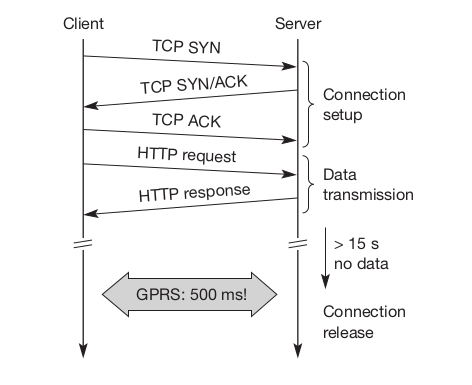
\includegraphics[width=0.8\textwidth]{tcp-connection-setup-overhead}
	\caption{Example TCP connection setup overhead}\label{fig:tcp_connection_setup_overhead}
\end{figure}


This led to the development of a transaction-oriented TCP (T/TCP). 
\begin{itemize}
	\item T/TCP can combine packets for connection establishment and connection release with user data packets. 
	\item This can reduce the number of packets down to two instead of seven.
\end{itemize}

\subsubsection{Advantages}
\paragraph*{Overhead Reduction}
The obvious advantage for certain applications is the reduction in the overhead which standard TCP has for connection setup and connection release. 

\subsubsection{Disadvantages}
\paragraph*{Requires Changes in MH and all CH}
T/TCP is not the original TCP anymore, so it requires changes in the mobile host and all correspondent hosts, which is a major disadvantage. 

\paragraph*{Mobility No Longer Transparent}
This solution no longer hides mobility. 

\paragraph*{Exhibits Several Security Problems}
Furthermore, T/TCP exhibits several security problems.


%%%%%%%%%%%%%%%%%%%%%%%%%%%%%
%							%
%		TABLE				%
%							%
%%%%%%%%%%%%%%%%%%%%%%%%%%%%%
\begin{landscape}
	\section[Classical Enhancements to TCP]{Overview of Classical Enhancements to TCP for Mobility}
	
\begin{longtable}[ht!]{@{}>{\raggedright\arraybackslash}p{3cm}>{\raggedright\arraybackslash}p{4.1cm}>{\raggedright\arraybackslash}p{4.1cm}>{\raggedright\arraybackslash}p{4.1cm}@{}}
	\caption{Overview of classical enhancements to TCP for mobility.}{\label{tab:classical_enhancments_tcp}} \\
	
	\toprule
	\textbf{Approach} & \textbf{Mechanism} & \textbf{Advantages} & \textbf{Disadvantages}\\
	\midrule
	
	\endfirsthead
	\multicolumn{2}{c}%
	{\tablename\ \thetable\ -- \textit{Continued from previous page}} \\
	
	\hline
	\textbf{Approach} & \textbf{Mechanism} & \textbf{Advantages} & \textbf{Disadvantages}\\
	\hline
	\endhead \hline
	\multicolumn{4}{r}{\textit{Continued on next page $\ldots$}} \\
	\endfoot
	\endlastfoot
	
	\textbf{Indirect TCP} & Splits TCP connection into two connections & Isolation of wireless link, simple & Loss of TCP semantics, higher latency at handover, security problems \tabularnewline
	
	\textbf{Snooping TCP} & Snoops data and acknowledgements, local retransmission & Transparent for end-to-end connection, MAC integration possible & Insufficient isolation of wireless link, security problems \tabularnewline
	

	\textbf{M-TCP} & Splits TCP connection, chokes sender via window size & Maintains end-to-end semantics, handles long term and frequent disconnections & Bad isolation of
	wireless link, processing overhead due to bandwidth management, security problems \tabularnewline


	\textbf{Fast retransmit/fast revcovery} & Avoids slow-start after roaming & Simple and
	efficient & Mixed layers, not transparent \tabularnewline


	\textbf{Transmission/time-out freezing} & Freezes TCP state at disconnection, resumes after reconnection & Independent of content, works for longer interruptions & Changes in TCP required, MAC dependent \tabularnewline

	\textbf{Selective retransmission} & Retransmits only lost data & Very effficient & Slightly more complex receiver software, more buffer space needed \tabularnewline


	\textbf{Transaction oriented TCP} & Combines connection setup/release and data transmission & Efficient for certain applications & Changes in TCP required,
	not transparent, security problems \tabularnewline
		
	\bottomrule
	
\end{longtable}
\end{landscape}
%
%
%Table \ref{tab:classical_enhancments_tcp} shows an overview of the classical mechanisms presented together with some advantages and disadvantages. The approaches are not all exclusive, but can be combined. Selective re-transmission, for example, can be used
%together with the others and can even be applied to fixed networks.
%
%An additional scheme that can be used to reduce TCP overhead is header
%compression. Using tunneling schemes as in mobile IP together with TCP, results in protocol headers of 60 byte in case of
%IPv4 and 100 byte for IPv6 due to the larger addresses. Many fields in the IP and
%TCP header remain unchanged for every packet. Only just transmitting the differences is often sufficient. Especially delay sensitive applications like, e.g.,
%interactive games, which have small packets benefit from small headers.
%However, header compression experiences difficulties when error rates are high
%due to the loss of the common context between sender and receiver.
%
%With the new possibilities of wireless wide area networks (WWAN) and their
%tremendous success, the focus of research has shifted more and more towards
%these 2.5G/3G networks. Up to now there are no final solutions to the problems
%arising when TCP is used in WWANs. However, some guidelines do exist.
%

\section{TCP over 2.5G/3G Wireless Networks}
The TCP over 2.5G/3G wireless networks describes a profile for optimizing TCP over wireless \gls{wan}s such as \gls{gsm}, \gls{gprs}, \gls{umts}. The focus on 2.5G/3G for transport of internet data is important as already billions of people use mobile phones and it is obvious that the mobile phone systems will also be used to transport arbitrary internet data.

\subsection[Characteristics]{Characteristics to be Considered}{\label{sec:characteristics_2_3_g}}
The following characteristics have to be considered when deploying applications over 2.5G/3G wireless links:

\subsubsection{Data Rates}
Typically, data rates are asymmetric as it is expected that users will download more data compared to uploading. Uploading is limited by the limited battery power. In cellular networks, asymmetry does not exceed 3–6 times, however, considering broadcast systems as additional distribution media (digital radio, satellite systems), asymmetry may reach a factor of 1,000.

\subsubsection{Latency}
All wireless systems comprise elaborated algorithms for error correction and protection, such as \gls{fec}, checksumming, and interleaving. FEC and interleaving let the \gls{rtt} grow to several hundred milliseconds up to some seconds.


\subsubsection{Jitter}
Wireless systems suffer from large delay variations or \textit{delay spikes}. Reasons for sudden increase in the latency are: 
\begin{itemize}
	\item link outages due to temporal loss of radio coverage,
	\item blocking due to high-priority traffic, or handovers
\end{itemize}

Handovers are quite often only virtually seamless with outages reaching from some $ 10 ms $ to several seconds.

\subsubsection{Packet Loss}
Packets might be lost during handovers or due to corruption. Due to link-level re-transmissions the loss rates of 2.5G/3G systems due to corruption are relatively low (but still orders of magnitude higher than, e.\ g.\, fiber connections). However, recovery at the link layer appears as \textit{jitter} to the higher layers.


\subsection[Configuration Parameters]{Configuration Parameters to Adapt TCP to Wireless Environments}

Based on the characteristics (see Section \ref{sec:characteristics_2_3_g}), configuration parameters to adapt TCP to wireless environments are:

\subsubsection{Large Windows}
TCP should support large enough window sizes based on the bandwidth delay experienced in wireless systems. With the help of the windows scale option and larger buffer sizes this can be accomplished. A larger initial window segments may increase performance particularly for short transmissions.


\subsubsection{Limited Transit}
This mechanism is an extension of Fast Re-transmission/Fast Recovery and is particularly useful when small amounts of data are to be transmitted (standard for, e.\ g.\, web service requests).

\subsubsection{Large MTU}
The larger the MTU (Maximum Transfer Unit) the faster TCP increases the congestion window. Large MTUs may be used to increase performance. MTU path discovery should be used to employ larger segment sizes instead of assuming the small default MTU.


\subsubsection[Selective Acknowledgment]{Selective Acknowledgment (SACK)}
SACK allows the selective re-transmission of packets and is almost always beneficial compared to the standard cumulative scheme.


\subsubsection[Explicit Congestion Notification]{Explicit Congestion Notification (ECN)}
ECN allows a receiver to inform a sender of congestion in the network by setting the ECN-Echo flag on receiving an IP packet that has experienced congestion. This mechanism makes it easier to distinguish packet loss due to transmission errors from packet loss due to congestion.


\subsubsection{Timestamp}
With the help of timestamps higher delay spikes can be tolerated by TCP without experiencing a spurious timeout. The effect of bandwidth oscillation is also reduced.

\subsubsection{No Header Compression}
Header compression is not compatible with TCP options such as SACK or timestamps.

 % Chapter-5: Mobile Transport Layer



% questions
\cleardoublepage
\phantomsection
\addcontentsline{toc}{chapter}{Questions (2018 \& 2019)}

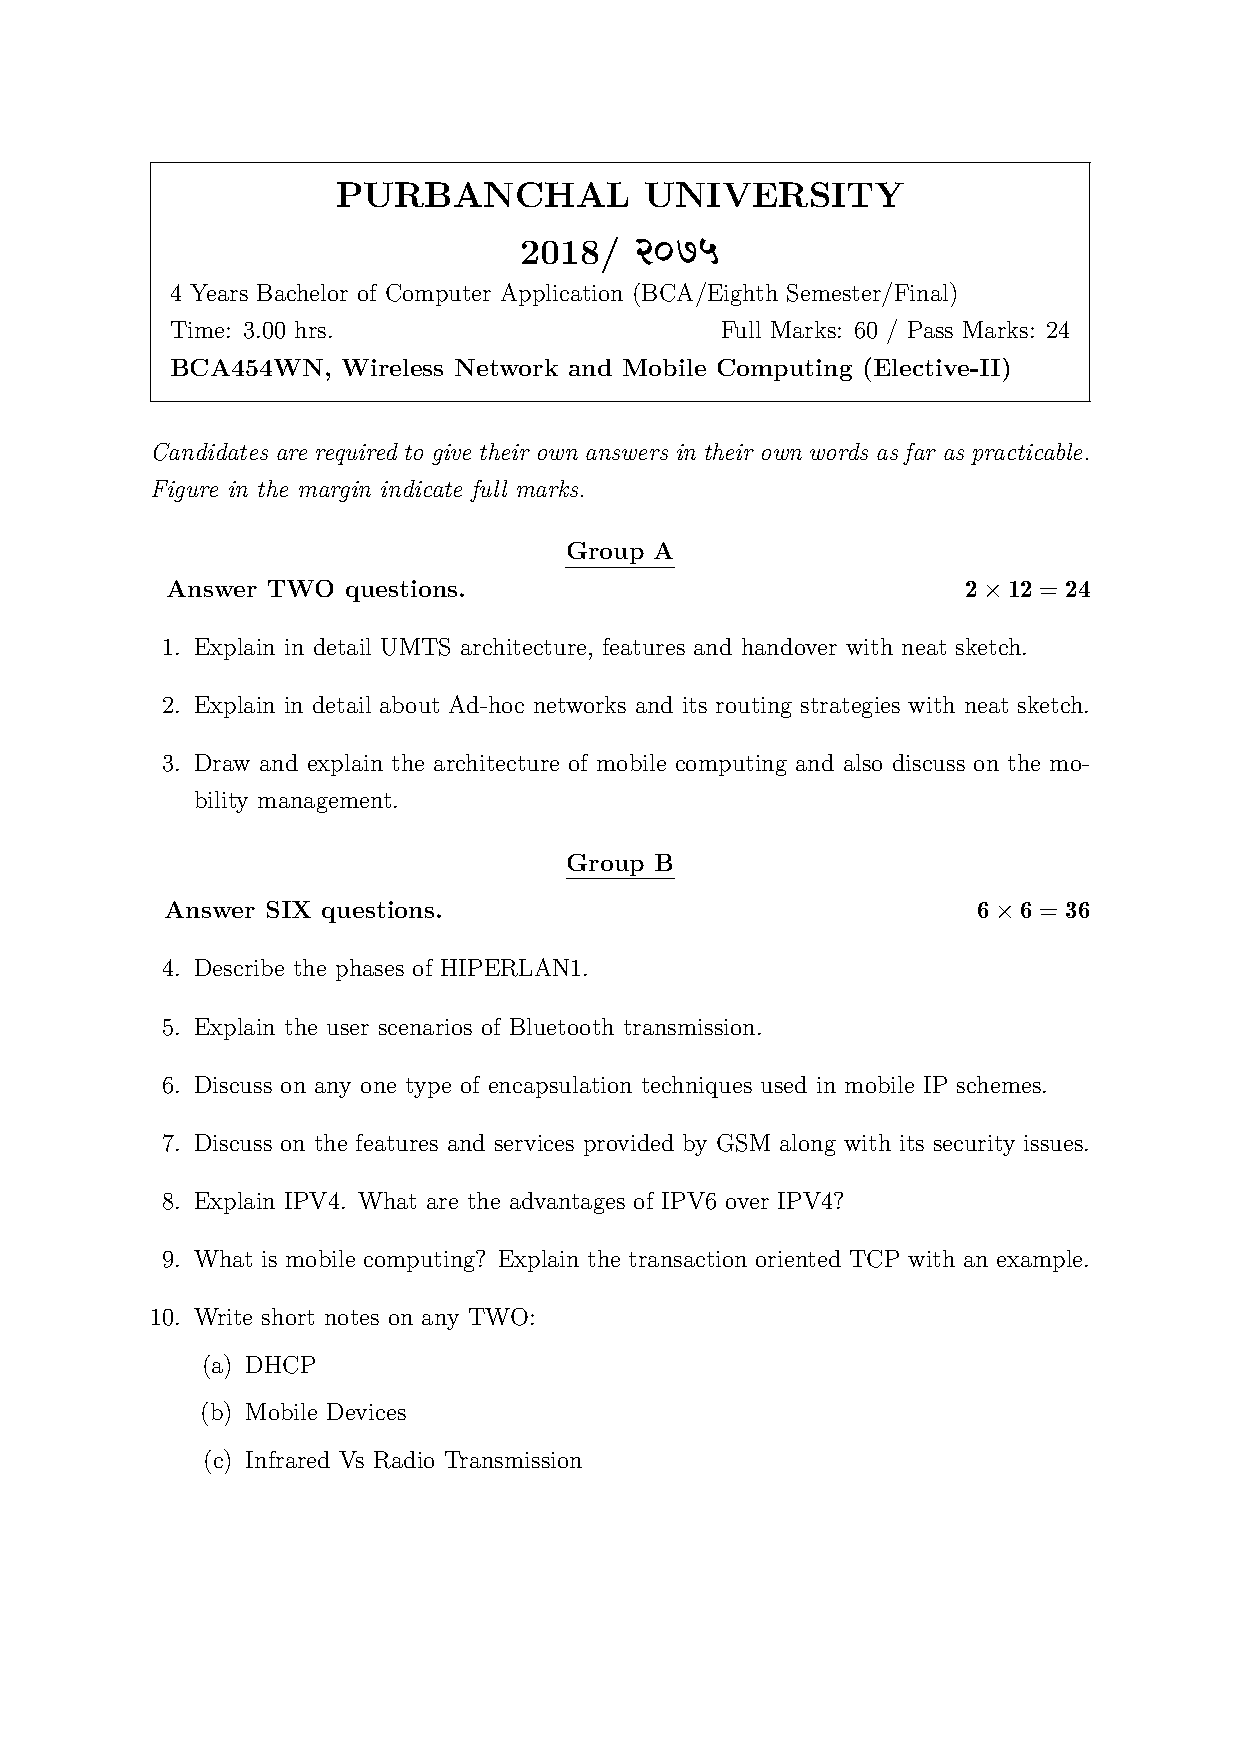
\includepdf[pagecommand={\thispagestyle{plain}}, pages={1-2}, scale=1.00]{./questions/wireless_networks_and_mobile_computing}



\backmatter

\nocite{*}
\renewcommand{\bibname}{Bibliography}
\phantomsection
\addcontentsline{toc}{chapter}{References}% add this to toc
\printbibliography %prints bibliography list


\end{document}
